\documentclass[11pt, a4paper, oneside]{Thesis} % Paper size, default font size and one-sided paper
\usepackage{wrapfig}
\usepackage{lscape}
\usepackage{rotating}
\usepackage{graphicx}
\usepackage{caption}
\usepackage{amsmath}
\usepackage{amssymb}
\usepackage{booktabs}
\usepackage{pifont}
\usepackage{array}
\usepackage{multirow}
% theorem / lemma / corollary / remark environments are defined in Thesis.cls


%\usepackage{subcaption} %incompatible with subfig
\usepackage[square, numbers]{natbib} % Use the natbib reference package - read up on this to edit the reference style; if you want text (e.g. Smith et al., 2012) for the in-text references (instead of numbers), remove 'numbers' v

\hypersetup{urlcolor=black, colorlinks=true} % Colors hyperlinks in blue - change to black if annoyingv`	
\title{\ttitle} % Defines the thesis title - don't touch this





%======================================================================|
%\thesistitle{An Approach to Writing a Thesis\\[3mm] for MDes at IIITDM}
\thesistitle{CausalTrace: Runtime Container Defense via Kernel Invariants and Sheaf Coupling}
\degree{B.Tech. Computer Science and Engineering }
\authors{Shubhankar Bhattacharya \\[-2mm] (Roll No: 122CS0047) \\[2mm]
         Anmol Kashyap \\[-2mm] (Roll No: 122CS0039)}
\supervisor{Dr.\ Anil Kumar R \\[-1mm] Assistant Professor (Grade-I)}
\department{Department of Computer Science and Engineering}
\DEPARTMENT{Department of Computer Science and Engineering}
%======================================================================|


\tolerance=1
\emergencystretch=\maxdimen
\hyphenpenalty=10000
\hbadness=10000


%======================================================================|
\begin{document}
\makeatletter
\renewcommand*{\NAT@nmfmt}[1]{\textsc{#1}}
\makeatother

% prints author names as small caps


\frontmatter % Use roman page numbering style (i, ii, iii, iv...) for the pre-content pages

\setstretch{1.6} % Line spacing of 1.6 (double line spacing)

% Define the page headers using the FancyHdr package and set up for one-sided printing
\fancyhead{} % Clears all page headers and footers
\rhead{\thepage} % Sets the right side header to show the page number
\lhead{} % Clears the left side page header

\pagestyle{fancy} % Finally, use the "fancy" page style to implement the FancyHdr headers

\newcommand{\HRule}{\rule{\linewidth}{0.5mm}} % New command to make the lines in the title page

% PDF meta-data
\hypersetup{pdftitle={\ttitle}}
\hypersetup{pdfsubject=\subjectname}
\hypersetup{pdfauthor=\authornames}
\hypersetup{pdfkeywords=\keywordnames}

%----------------------------------------------------------------------------------------
%	TITLE PAGE
%----------------------------------------------------------------------------------------

\begin{titlepage}
\begin{center}


%\HRule \\[0.4cm] % Horizontal line
\vspace{0.4cm} % Horizontal line
{\huge \bfseries \ttitle}\\[0.4cm] % Thesis title
%\HRule \\[1.5cm] % Horizontal line
\vspace{1.5cm} % Horizontal line

 
\large \textit{A report submitted in partial fulfilment of the requirements\\ for the award of the degree of \\ B.Tech Computer Science and Engineering }\\[0.3cm] % University requirement text
\textit{by}\\[0.4cm]

\authornames

\vfill
\graphicspath{ {./Figures/} }
\begin{figure}[hb]
  \centering
  
\includegraphics[width=0.3\linewidth]{klogo.png}
\end{figure}

\DEPTNAME\\ % Research group name and department name
\textsc{ \UNIVNAME}\\[1.5cm] % University name
\large April 2026\\[2cm] % Date


\end{center}

\end{titlepage}

%----------------------------------------------------------------------------------------
%	EVALUATION SHEET
%----------------------------------------------------------------------------------------

\Evaluation{\addtocontents{toc}{\vspace{1em}}

\vspace{8mm}

\noindent\textbf{Title of the Project:}\\[2mm]
CausalTrace: Runtime Container Defense via Kernel Invariants and Sheaf
Coupling

\vspace{8mm}

\noindent\textbf{Name of the Student:}
\begin{itemize}
    \item Shubhankar Bhattacharya (Roll No: 122CS0047)\\[-10mm]
    \item Anmol Kashyap (Roll No: 122CS0039)
\end{itemize}

\vspace{10mm}

\noindent\textbf{Examiner(s):}\\[2mm]
\rule{8cm}{0.4pt}

\vspace{10mm}

\noindent\textbf{Supervisor/Advisor:}\\[2mm]
\rule{8cm}{0.4pt}

\vspace{10mm}

\noindent\textbf{Head of the Department:}\\[2mm]
\rule{8cm}{0.4pt}

\vspace{10mm}

\noindent\textbf{Date:} \rule{4cm}{0.4pt}

\vspace{5mm}

\noindent\textbf{Place:} \rule{4cm}{0.4pt}

}

\clearpage

%----------------------------------------------------------------------------------------
%	DECLARATION PAGE
%	Your institution may give you a different text to place here
%----------------------------------------------------------------------------------------


\Declaration{\addtocontents{toc}{\vspace{1em}} % Add a gap in the Contents, for aesthetics


%\begin{center}
%\LARGE{\underline{\textbf{Declaration of Originality}}}
%\end{center}
\noindent We, the undersigned students, hereby declare that the material presented
in the Project Report titled \textit{``CausalTrace: Runtime Container Defense
via Kernel Invariants and Sheaf Coupling''} represents original work carried
out by us
in the Department of Computer Science and Engineering at the Indian Institute
of Information Technology, Design and Manufacturing, Kurnool during the
academic year \textbf{2025--2026}. With our signatures, we certify that:
\begin{itemize}
    \item We have not manipulated any of the data or results.\\[-10mm]
    \item We have not committed any plagiarism of intellectual
          property.\\[-10mm]
    \item We have clearly indicated and referenced the contributions of
          others.\\[-10mm]
    \item We have explicitly acknowledged all collaborative research
          and discussions.\\[-10mm]
    \item We understand that any false claim will result in severe
          disciplinary action.\\[-10mm]
    \item We understand that the work may be screened for any form
          of academic {misconduct}.
\end{itemize}

\vspace{10mm}

\noindent\begin{tabular}{@{}p{0.55\textwidth}p{0.35\textwidth}@{}}
Shubhankar Bhattacharya (122CS0047) & Signature \\[6mm]
Anmol Kashyap (122CS0039)           & Signature \\
\end{tabular}

\vspace{6mm}

\noindent Date: \rule{4cm}{0.4pt}

\vspace{10mm}

\noindent In my capacity as supervisor of the above-mentioned work, I certify
that the work presented in this Report is carried out under my supervision,
and is worthy of consideration for the requirements of B.Tech.\ Project work.

\vspace{10mm}

\noindent Supervisor's Name: \textbf{Dr.\ Anil Kumar R} \hfill Supervisor's Signature:
\rule{4cm}{0.4pt}
}

%----------------------------------------------------------------------------------------
%	ABSTRACT PAGE
%----------------------------------------------------------------------------------------

\addtotoc{Abstract} % Add the "Abstract" page entry to the Contents

\abstract{\addtocontents{toc}{\vspace{1em}}

Runtime security for containerised workloads sits between two surfaces: the
kernel, which observes every syscall, and the user-space control plane,
which observes none of them fast enough to matter. Rule-based eBPF agents
such as Falco and Tetragon read single syscalls in isolation and flag
payloads; they cannot see the \emph{edges} of a multi-step chain that
pivots between containers.

This thesis presents \textbf{CausalTrace}, a three-tier runtime defence
built to close that gap. Tier~1 attaches a tail-call dispatcher to the raw
\texttt{sys\_enter} tracepoint and drives six in-kernel invariant
handlers---fork acceleration, execve, sensitive-file, privilege escalation,
a \texttt{dup2} file-descriptor-type check, and namespace transition. A
compound gate routes each breach through a strict, self-inflicted, or
trust-gated case, and burns the attacker's IP into a TC classifier that
drops their packets at the veth. Tier~2 stitches accepted TCP flows to
their remote peer and promotes trust on an L4-stability test. Tier~3
projects each container's syscall bigram into a 74-dimensional signal,
applies canonical-correlation restriction maps at rank $k=15$, and
computes Mahalanobis edge energies plus a global Rayleigh quotient over a
cellular sheaf Laplacian. Four theorems tie the approach to the system:
invariant necessity, bigram-noise adversarial closure, two-layer
completeness, and trust-promotion soundness.

Evaluation replays a fixed-seed permutation of 155 attack injections
(150~in-distribution drawn from eleven classes, 5 held-out
\texttt{memfd\_create} fileless payloads) against every detector under an
identical workload on a 22-container mesh. CausalTrace catches 154 of the
155 injections (99.4\,\% [96, 100]); Falco tuned reaches 70.3\,\% [63, 77]
and Tetragon tuned reaches 1.3\,\% [0, 5]. Cross-container lateral
movement, chained SSRF~$\rightarrow$~RCE, and fileless out-of-distribution
payloads are detected at 100\,\% while every rule-based baseline misses
them entirely. Chapter~\ref{Chapter6} reports the full per-scenario
breakdown with Wilson 95\,\% confidence intervals.
}

\clearpage % Start a new page

%----------------------------------------------------------------------------------------
%	ACKNOWLEDGEMENTS
%----------------------------------------------------------------------------------------

\setstretch{1.3} % Reset the line-spacing to 1.3 for body text (if it has changed)

\acknowledgements{\addtocontents{toc}{\vspace{1em}} % Add a gap in the Contents, for aesthetics

We extend our sincere thanks to our supervisor Dr.\ Anil Kumar R,
Assistant Professor (Grade-I), Department of Computer Science and
Engineering, IIITDM Kurnool, for his guidance, patience, and the regular
reviews that kept this project on course through its full length. His
feedback at every stage improved both the technical direction of the work
and the clarity of its presentation.

We also thank the Department of Computer Science and Engineering and the
Indian Institute of Information Technology, Design and Manufacturing,
Kurnool, for providing the academic environment in which this project was
undertaken. We are thankful to our families for their constant support,
and to our peers for the many discussions that shaped this work along the
way. Any errors that remain are ours.

}
\clearpage % Start a new page

%----------------------------------------------------------------------------------------
%	LIST OF CONTENTS/FIGURES/TABLES PAGES
%----------------------------------------------------------------------------------------

\pagestyle{fancy} % The page style headers have been "empty" all this time, now use the "fancy" headers as defined before to bring them back

\lhead{\emph{Contents}} % Set the left side page header to "Contents"
\tableofcontents % Write out the Table of Contents

\lhead{\emph{List of Figures}} % Set the left side page header to "List of Figures"
\listoffigures % Write out the List of Figures

\lhead{\emph{List of Tables}} % Set the left side page header to "List of Tables"
\listoftables % Write out the List of Tables

%----------------------------------------------------------------------------------------
%	ABBREVIATIONS
%----------------------------------------------------------------------------------------

\clearpage % Start a new page

\setstretch{1.5} % Set the line spacing to 1.5, this makes the following tables easier to read

\lhead{\emph{Abbreviations}} % Set the left side page header to "Abbreviations"
\listofsymbols{ll} % Include a list of Abbreviations (a table of two columns)
{
\textbf{BCC}   & \textbf{B}PF \textbf{C}ompiler \textbf{C}ollection \\
\textbf{BPF}   & \textbf{B}erkeley \textbf{P}acket \textbf{F}ilter \\
\textbf{CCA}   & \textbf{C}anonical \textbf{C}orrelation \textbf{A}nalysis \\
\textbf{CMS}   & \textbf{C}ount-\textbf{M}in \textbf{S}ketch \\
\textbf{eBPF}  & \textbf{e}xtended \textbf{B}erkeley \textbf{P}acket \textbf{F}ilter \\
\textbf{FPR}   & \textbf{F}alse \textbf{P}ositive \textbf{R}ate \\
\textbf{kprobe}& \textbf{K}ernel \textbf{Probe} \\
\textbf{LSM}   & \textbf{L}inux \textbf{S}ecurity \textbf{M}odule \\
\textbf{LRU}   & \textbf{L}east \textbf{R}ecently \textbf{U}sed \\
\textbf{PCA}   & \textbf{P}rincipal \textbf{C}omponent \textbf{A}nalysis \\
\textbf{OOD}   & \textbf{O}ut-\textbf{o}f-\textbf{D}istribution \\
\textbf{TC}    & \textbf{T}raffic \textbf{C}ontrol (Linux) \\
\textbf{TID}   & \textbf{T}hread \textbf{ID} \\
\textbf{TPR}   & \textbf{T}rue \textbf{P}ositive \textbf{R}ate \\
}

%----------------------------------------------------------------------------------------
%	PHYSICAL CONSTANTS/OTHER DEFINITIONS
%----------------------------------------------------------------------------------------
%
%\clearpage % Start a new page
%
%\lhead{\emph{Physical Constants}} % Set the left side page header to "Physical Constants"
%
%\listofconstants{lrcl} % Include a list of Physical Constants (a four column table)
%{
%Speed of Light & $c$ & $=$ & $2.997\ 924\ 58\times10^{8}\ \mbox{ms}^{-\mbox{s}}$ (exact)\\
%% Constant Name & Symbol & = & Constant Value (with units) \\
%}

%----------------------------------------------------------------------------------------
%	SYMBOLS
%----------------------------------------------------------------------------------------

\clearpage % Start a new page

\lhead{\emph{Symbols}} % Set the left side page header to "Symbols"

\listofnomenclature{lll} % Include a list of Symbols (a two column table)
{
$L_F$        & cellular sheaf Laplacian over the container graph \\
$R(x)$       & global Rayleigh quotient $x^{\!\top}\!L_F x\,/\,x^{\!\top}\!x$ \\
$\tau$       & per-edge Mahalanobis threshold (mean $+\,4\sigma$) \\
$\tau_{\text{global}}$ & calibrated Rayleigh threshold \\
$d=74$       & sheaf signal dimension per container \\
$k=15$       & CCA restriction-map rank \\
$\alpha=0.02$& EMA smoothing factor \\
$B,\Delta$   & bytes-budget and duration gate for trust promotion \\
}

%----------------------------------------------------------------------------------------
%	DEDICATION
%----------------------------------------------------------------------------------------
%
\setstretch{1.3} % Return the line spacing back to 1.3
%
\addtocontents{toc}{\vspace{2em}} % Add a gap in the Contents, for aesthetics

%----------------------------------------------------------------------------------------
%THESIS CONTENT - CHAPTERS
%----------------------------------------------------------------------------------------
\mainmatter % Begin numeric (1,2,3...) page numbering
\pagestyle{fancy} 


\chapter{Introduction}
\label{Chapter1}
\lhead{Chapter 1. \emph{Introduction}}

A production Kubernetes node shares a single Linux kernel among tens to
hundreds of containers. That kernel is a shared fate~\cite{gregg2019bpf}: one
race in namespace teardown, one off-by-one in \texttt{copy\_from\_user}, one
exploitable path in \texttt{io\_uring}---any of these hands every co-tenant on
the node to the attacker at once. Container isolation is a policy, not a
hardware boundary. It holds until it does not.

This thesis is about the attacks that never need to break that boundary. They
walk between containers through syscalls the kernel is already allowed to
serve. Each hop reads as benign under any local per-container policy, yet the
composition is a credential exfiltration, a lateral pivot, a container
escape. The work reported here builds a three-tier runtime defence that
treats such compositions as first-class: not deviations from a single
container's profile, but \emph{edges} in a graph that the kernel can
instrument directly.

%─────────────────────────────────────────────────────────────────────────────
\section{The shared-kernel attack surface}
\label{sec:attack-surface}
%─────────────────────────────────────────────────────────────────────────────

Modern microservice deployments layer an externally reachable tier (a web
front-end, an API gateway) over an internal tier (databases, caches, message
queues) that the outer tier reaches over a flat overlay network. Both layers
share the same kernel, the same cgroup hierarchy, and the same BPF map space.

Consider a concrete chain on the evaluation testbed: \texttt{ct\_attacker}
exploits a server-side request forgery in \texttt{ct-nginx}, which proxies a
crafted request to \texttt{ct-api-gw} on port 8080. The gateway, processing
what it reads as a legitimate upstream call, queries \texttt{ct-postgres} on
port~5432. Each individual syscall along the way---\texttt{connect(2)},
\texttt{sendmsg(2)}, \texttt{recvmsg(2)}---is permitted by any reasonable
per-container policy. The anomaly lives entirely in the \emph{edge} between
containers, not in any single container's syscall trace.

Existing open-source defences miss this class of attack by design.
Falco~\cite{falco2024} matches per-container syscall sequences against a rule
library; it fires on payloads. Tetragon~\cite{tetragon2024} attaches kprobes
and enforces per-pod network policies. Tracee~\cite{tracee2024} builds
per-process behaviour profiles. None of the three model the relationship
\emph{between} containers.

%─────────────────────────────────────────────────────────────────────────────
\section{Why per-container detectors are blind to composite attacks}
\label{sec:bosc-blindness}
%─────────────────────────────────────────────────────────────────────────────

The dominant IDS paradigm for containers is a variant of
Bag-of-System-Calls~(BoSC)~\cite{bertinatto2024,kotenko2024}: build a
frequency or sequence profile of the syscalls a container issues under normal
operation, then flag deviations at runtime. These detectors are lightweight
and interpretable. Their weakness is semantic. They observe \emph{what} a
container does, not \emph{why} or \emph{in response to whom}.

We showed this empirically during mid-review. The same
\texttt{openat("/etc/passwd")} is benign when \texttt{apt-get} resolves a
user-ID and malicious when a compromised worker reads credentials. The same
\texttt{clone(2)} burst is benign when \texttt{gpgv} verifies package
signatures and malicious during a fork bomb. The same \texttt{setuid(0)} is
required by \texttt{runc} during container init and forbidden during request
handling~\cite{ghimire2025patrol}. Every benign case forces a whitelist entry into
any rule-based detector. Every whitelist entry becomes an evasion vector.

The deeper failure mode is multi-hop composition. Suppose an attacker chain
runs: shell spawn in \texttt{ct-webapp-a}, lateral connect to
\texttt{ct-api-gw} on an uncalibrated port, further connect to
\texttt{ct-postgres}~\cite{he2023cross}. Each container produces a locally
plausible trace. The attack is encoded in the \emph{joint} behaviour of the
trio---in the fact that the shell-spawn and the lateral connect occurred
inside the same five-second window in the same cgroup, and that the
downstream container then opened a connection it had never opened during
calibration. Standard BoSC tooling cannot see that joint behaviour; it lacks
the mathematical object---a global model of how containers are \emph{supposed
to} couple---that would encode it.

\begin{figure}[t]
  \centering
  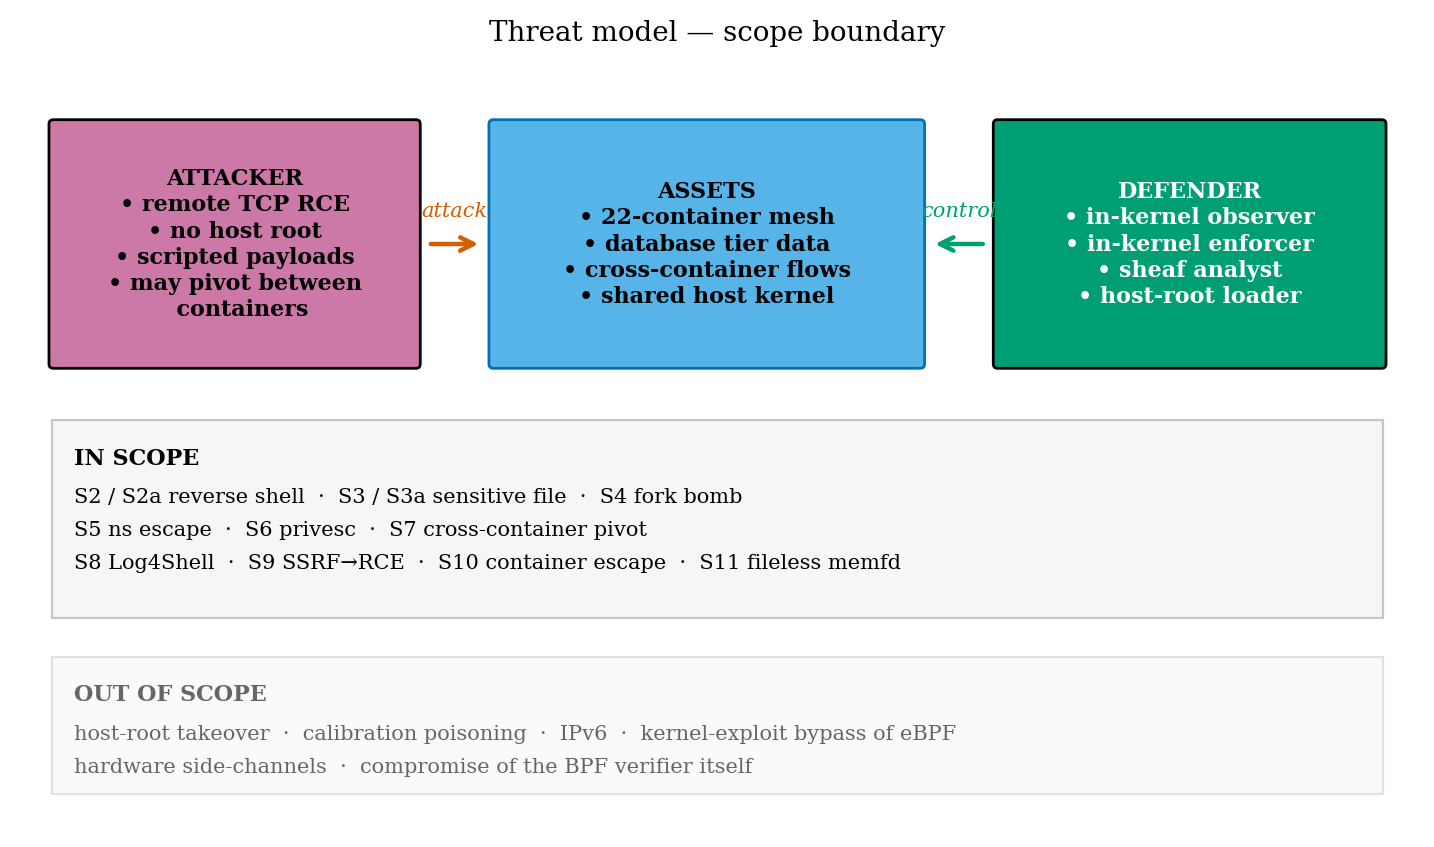
\includegraphics[width=0.92\linewidth]{figures/fig_threat_model.png}
  \caption[Thesis scope boundary]{Scope of the defence. Every attack in the
  in-scope band is either a physical kernel invariant (caught by Tier~1) or a
  cross-container edge anomaly (caught by Tier~3). The out-of-scope band lists
  assumptions that are standard for this class of system.}
  \label{fig:intro-scope}
\end{figure}

%─────────────────────────────────────────────────────────────────────────────
\section{Problem statement}
\label{sec:problem}
%─────────────────────────────────────────────────────────────────────────────

\textbf{Problem.} Design, implement, and evaluate a container security
system that
\begin{enumerate}
  \item enforces physical syscall invariants at sub-microsecond latency with
        no user-space decision in the kill path,
  \item attributes every accepted network byte to the client IP that caused
        it, so enforcement is \emph{surgical}---one attacker IP is severed
        rather than the entire container process being killed,
  \item detects novel cross-container attack chains that no per-container
        IDS can see, using a principled mathematical model of inter-container
        coupling, and
  \item sustains a realistic concurrent workload with measurable, bounded
        overhead, producing detection rates with tight confidence intervals
        against Falco and Tetragon baselines on the same host.
\end{enumerate}

%─────────────────────────────────────────────────────────────────────────────
\section{Contributions}
\label{sec:contributions}
%─────────────────────────────────────────────────────────────────────────────

This thesis makes four contributions.

\paragraph{A three-tier architecture with a strict dependency rule.}
Tier~1 (kernel, 6 eBPF handlers) enforces kernel invariants inline on
\texttt{sys\_enter}. Tier~2 (kprobe on \texttt{inet\_csk\_accept} plus a TC
classifier) attributes every accepted byte to a client IP and severs the
attacker session at the veth by dropping their packets on an expiring BPF
map. Tier~3 (Python daemon) computes a 74-dimensional signal per container
per five-second window and passes it through a cellular sheaf Laplacian. The
dependency rule is asymmetric: Tier~1 never blocks on Tier~3.

\paragraph{TC-drop session severance.}
Earlier prototypes called \texttt{bpf\_send\_signal(9)} against the container
process, which terminated every live connection the container was serving.
We replace this with a \texttt{drop\_ip\_list} BPF map (key: IPv4 source,
value: \texttt{CLOCK\_MONOTONIC} expiry) read by the TC ingress and egress
classifiers on each veth. Only packets to or from the burned IP are dropped;
other clients are untouched. A five-minute TTL self-heals false positives
without operator intervention.

\paragraph{A rank-15 CCA calibration that fits real calibration windows.}
An earlier iteration of the pipeline fitted CCA at $k=50$ and produced
rank-deficient restriction maps whenever a calibration window contained
fewer than sixty aligned samples per edge. We show that $k=15$ keeps every
edge well-conditioned at realistic calibration durations on our 22-container
testbed and eliminates the false-positive storm that a rank-deficient
covariance inversion causes at runtime.

\paragraph{A seed-reproducible evaluation harness.}
A fixed random permutation of 150 in-distribution attack injections (drawn
from eleven classes) plus five held-out \texttt{memfd\_create} out-of-
distribution injections is replayed identically against CausalTrace, Falco
(stock and tuned), and Tetragon (stock and tuned) under the same concurrent
background load. The harness produces per-scenario Wilson 95\,\% confidence
intervals~\cite{wilson1927}, detection-latency cumulative distributions, and
per-syscall overhead. Chapter~\ref{Chapter6} reports the results.

\chapter{Literature Review and Research Gaps}
\label{Chapter2}
\lhead{Chapter 2. \emph{Literature Review and Gaps}}

Prior work on container runtime security falls into four groups: production
rule engines, anomaly-based syscall detectors, in-kernel enforcers, and
cross-container research. Each group solves a real problem, and each leaves
a specific gap that CausalTrace is engineered to close. We frame the review
around those gaps.

%─────────────────────────────────────────────────────────────────────────────
\section{Production runtime security tools}
\label{sec:lit-production}
%─────────────────────────────────────────────────────────────────────────────

Three open-source tools dominate the production market. Falco~\cite{falco2024}
matches kernel events against a YAML rule library through a modern-eBPF
probe. Tetragon~\cite{tetragon2024}, a sub-project of
Cilium~\cite{cilium2024}, compiles \emph{TracingPolicies} to eBPF kprobes and
supports in-kernel enforcement through signal delivery and socket override.
Tracee~\cite{tracee2024} focuses on forensics: it emits events for post-hoc
analysis rather than enforcing in the hot path.

All three operate on per-container streams. Rules match inside one
container's own syscall trace or against a deny-list; there is no primitive
that expresses \emph{container $A$ spawns a shell within five seconds of
container $B$ connecting to a previously-unseen port}. A correlation layer
can be built on top of any of them, but the round-trip to userspace that
the layer forces up wipes out the latency advantage that in-kernel detection
was supposed to provide.

Ghimire~\emph{et al.}~\cite{ghimire2025patrol} (eBPF-PATROL) are the closest
published baseline to our Tier~1 design. They intercept six dangerous
syscalls (\texttt{clone}, \texttt{execve}, \texttt{openat}, \texttt{setns},
\texttt{unshare}, \texttt{ptrace}) and enforce through BPF LSM hooks at
$\sim$100\,ns and \texttt{bpf\_override\_return} at $\sim$200\,ns. They
miss the same cross-container class that Falco and Tetragon miss, and they
require a twelve-entry infrastructure whitelist (documented by them and
reproduced in our own mid-review) to keep Docker's own runtime from
tripping the rules.

%─────────────────────────────────────────────────────────────────────────────
\section{Anomaly-based syscall detectors}
\label{sec:lit-bosc}
%─────────────────────────────────────────────────────────────────────────────

The Bag-of-System-Calls (BoSC) family represents a container's behaviour as
a frequency vector over syscall opcodes. Bertinatto~\emph{et
al.}~\cite{bertinatto2024} attach a raw tracepoint to \texttt{sys\_enter},
filter by mount namespace, and build per-process BoSC vectors. The method
cleanly catches one hardcoded container-escape pattern
(\texttt{openat("/proc/1/ns/mnt")} followed by
\texttt{setns(CLONE\_NEWNS)}) and misses every other class of attack.

Autoencoder-based detectors~\cite{kotenko2024,desilva2022micro,xia2024selfsup}
and sequence models~\cite{chen2021lstm,fournier2023lm} lift this work by
learning a density estimate over benign traces. They share the structural
weakness: the model learns the \emph{marginal} distribution per container
but not the joint structure between containers, so an attacker whose
individual syscall frequencies stay close to the marginal can compose an
attack whose joint signature is far from any single container's
calibrated regime.

%─────────────────────────────────────────────────────────────────────────────
\section{In-kernel enforcement and adversarial evasion}
\label{sec:lit-enforcement}
%─────────────────────────────────────────────────────────────────────────────

A smaller body of work targets enforcement in kernel space. Zhang~\emph{et
al.}~\cite{zhang2024rtids} build a neural-network inference engine that
runs inside eBPF through tail calls and integer arithmetic, reporting F1
scores of 0.933 and 0.992 on packet-level intrusion datasets with 5\,KB of
in-kernel memory. The design is elegant at the verifier boundary, but the
detection target is packet flows, not multi-container chains.

Takabayashi and Mambo~\cite{takabayashi2024evasion} study the adversarial
other side: how an attacker can \emph{evade} eBPF-based detectors by
\texttt{LD\_PRELOAD}-rewriting syscall arguments, hiding process files
through \texttt{getdents} rewriting, or dropping payload packets through
XDP. Their evasion results motivate the strict-invariant design
philosophy of CausalTrace's Tier~1: we hook on physical contract violations
(a process whose standard input points to a socket is a reverse shell) that
the attacker cannot semantically rewrite away.

%─────────────────────────────────────────────────────────────────────────────
\section{Cross-container attack research}
\label{sec:lit-cross}
%─────────────────────────────────────────────────────────────────────────────

He~\emph{et al.}~\cite{he2023cross} document the cross-container attack
class. They catalogue five vulnerable online services in which offensive
eBPF features break container isolation, and three cloud providers' default
Kubernetes clusters vulnerable to cross-node attacks. Their contribution is
attack discovery; they propose no defender.

Zhang~\emph{et al.}~\cite{zhang2025path} (Pamir-Detector) monitors
path-resolution syscalls for filesystem-isolation bypasses (symlink attacks,
procfs traversal, host-process-mediated file access). Their coverage is
one escape family; CausalTrace's Tier~1 handlers cover complementary
families (socket-stdio reverse shells, namespace manipulation, setuid-0
from non-root). No published defender models the joint behaviour of
multiple containers mathematically and detects composite attacks that never
trip a single-container rule. That is the gap this thesis closes.

%─────────────────────────────────────────────────────────────────────────────
\section{Mathematical foundations}
\label{sec:lit-math}
%─────────────────────────────────────────────────────────────────────────────

The Tier~3 detector reuses four classical constructions as stated; no new
mathematical theorems about them are claimed.

Canonical-correlation analysis~\cite{hotelling1936} supplies the restriction
maps $F_u, F_v$ per edge of the communication graph. The Mahalanobis
distance~\cite{mahalanobis1936} scores residuals against the learned
coupling covariance. The Count-Min Sketch~\cite{cormode2005cms} gives our
in-kernel bigram counter at $4 \times 128$ per container. Cellular-sheaf
spectral theory~\cite{hansen2019spectral,curry2014sheaves,robinson2014topological}
provides the sheaf Laplacian~$L_F$ and the Rayleigh-quotient interpretation
as a coupling-consistency measure. The sheaf specialises to the ordinary
graph Laplacian of spectral graph theory~\cite{chung1997spectral} whenever
every restriction map is the identity.

%─────────────────────────────────────────────────────────────────────────────
\section{Capability matrix and research gaps}
\label{sec:gaps}
%─────────────────────────────────────────────────────────────────────────────

Table~\ref{tab:capability-matrix} summarises where each reviewed system sits
against the capabilities we consider essential for defending a composite
cross-container attack. A single row is filled in by CausalTrace.

\begin{table}[t]
\centering
\caption[Capability matrix of reviewed runtime security systems]
{Capabilities of reviewed runtime security systems. \ding{51}\,=\,full,
$\sim$\,=\,partial, \ding{55}\,=\,absent. $^{\dagger}$In-kernel enforcement
is possible via \texttt{bpf\_send\_signal} but is community-discouraged in
production because it terminates the entire container process.}
\label{tab:capability-matrix}
\footnotesize
\setlength\tabcolsep{3.5pt}
\begin{tabular}{@{}l c c c c c c@{}}
\toprule
System & Cross- & Kernel- & Sub-$\mu$s & OOD & No labelled & Attacker-IP \\
       & container & native enf. & latency & detect. & train data & severance \\
\midrule
Falco~\cite{falco2024}          & \ding{55} & \ding{55}$^{\dagger}$ & \ding{55} & \ding{55} & \ding{51} & \ding{55} \\
Tetragon~\cite{tetragon2024}    & \ding{55} & $\sim$    & \ding{51} & \ding{55} & \ding{51} & \ding{55} \\
Tracee~\cite{tracee2024}        & \ding{55} & \ding{55} & \ding{55} & \ding{55} & \ding{51} & \ding{55} \\
BoSC~\cite{bertinatto2024}      & \ding{55} & \ding{55} & \ding{55} & \ding{55} & \ding{55} & \ding{55} \\
eBPF-PATROL~\cite{ghimire2025patrol}
                                & \ding{55} & \ding{51} & \ding{51} & \ding{55} & \ding{51} & \ding{55} \\
LSTM~/~LM~\cite{chen2021lstm,fournier2023lm}
                                & \ding{55} & \ding{55} & \ding{55} & $\sim$    & \ding{55} & \ding{55} \\
Pamir-Detector~\cite{zhang2025path}
                                & \ding{55} & \ding{51} & \ding{51} & \ding{55} & \ding{51} & \ding{55} \\
\textbf{CausalTrace (this work)}
                                & \textbf{\ding{51}} & \textbf{\ding{51}}
                                & \textbf{\ding{51}} & \textbf{\ding{51}}
                                & \textbf{\ding{51}} & \textbf{\ding{51}} \\
\bottomrule
\end{tabular}
\end{table}

From this matrix and the preceding review we distil five research gaps.

\paragraph{G1 --- Semantic blindness of rule-based detectors.}
Baseline~B (our mid-review Modified PATROL) detected all five attack classes
but required twelve infrastructure whitelist entries
(\texttt{apt-get}, \texttt{gpgv}, \texttt{runc}, \texttt{containerd}, and
eight others) to keep normal Docker operations from tripping the rules. Each
entry is both a maintenance burden and an evasion vector. The gap is
semantic: identical syscalls have different intent depending on context,
and no amount of rule tuning closes a gap that lives in meaning rather than
syntax.

\paragraph{G2 --- No cross-container chain detection.}
Every reviewed defender operates on per-container events. Multi-stage
chains---Log4Shell in a webapp, Dirty-Pipe for privilege escalation, a
cgroup escape to the host---are invisible to a single-event monitor because
each stage is locally plausible. He~\emph{et al.}~\cite{he2023cross}
document the attack class and propose no defender.

\paragraph{G3 --- Userspace enforcement bottleneck.}
PATROL-class architectures route every decision through a userspace Go
controller: eBPF probe $\rightarrow$ ring buffer $\rightarrow$ controller
$\rightarrow$ \texttt{kill()}. Mid-review measurements on that path
recorded approximately $23\,\mu$s round-trip; the triggering syscall
completes before the kill arrives.

\paragraph{G4 --- Coarse enforcement target.}
Kernel-native enforcement delivered through \texttt{bpf\_send\_signal(SIGKILL)}
targets the container process itself. In a deployment serving legitimate
users alongside the attacker, this is collateral damage---every in-flight
request terminates the moment an invariant fires. No reviewed system
severs at attacker-IP granularity.

\paragraph{G5 --- No mathematical model of inter-container coupling.}
The object that encodes \emph{which containers may communicate, at what
cadence, and with what joint syscall distribution} is absent from every
reviewed system. BoSC operates on per-container marginals; network
detectors operate on per-flow features; neither captures the joint
structure that a sheaf Laplacian makes explicit.

Chapters~\ref{Chapter3}--\ref{Chapter6} close these five gaps, respectively
through the math, the architecture, the implementation, and the evaluation.
 
\chapter{Theoretical Framework}
\label{Chapter3}
\lhead{Chapter 3. \emph{Theoretical Framework}}

The Tier~3 detector runs a small mathematical pipeline every detection
cycle: a bigram sketch becomes a 74-dimensional signal, the signal is
projected into an edge-local coupling subspace by a CCA-learned restriction
map, Mahalanobis energy scores the edge, and a global Rayleigh quotient
over a cellular sheaf Laplacian scores the whole container graph. A guarded
exponential moving average keeps the global threshold honest under normal
drift without letting a slow-drip attack poison it.

We state the classical pieces as given and cite primary
sources~\cite{hotelling1936,mahalanobis1936,hansen2019spectral,curry2014sheaves,robinson2014topological,chung1997spectral}.
No new mathematics about these objects is claimed. The contribution of this
chapter is the assembly into a deployable detector and the four theorems in
Section~\ref{sec:theorems}, which capture why that assembly is hard to
evade.

%─────────────────────────────────────────────────────────────────────────────
\section{Notation}
\label{sec:notation}
%─────────────────────────────────────────────────────────────────────────────

$C = \{c_1, \ldots, c_n\}$ is the set of monitored containers, each with
cgroup identifier $g_i \in \mathbb{N}$. A detection cycle is a window of
length $T$ indexed by $t$. At cycle $t$ each container produces a signal
$\mathbf{x}_i^{(t)} \in \mathbb{R}^d$ with $d = 74$. The communication graph
$G = (V, E)$ has $V = C$ and $E$ the set of observed inter-container edges;
we write $e = (u, v, \ell)$ with $\ell \in \{0,1,2\}$ encoding the temporal
lag. After calibration every edge carries restriction maps
$F_u^{(e)}, F_v^{(e)} \in \mathbb{R}^{k \times d}$ with $k = 15$, a
regularised covariance $\Sigma_e \in \mathbb{R}^{k \times k}$, and a
Mahalanobis threshold $\tau_e$. The global Rayleigh threshold is
$\tau_{\text{global}}$.

%─────────────────────────────────────────────────────────────────────────────
\section{Bigram sketch and the 74-dimensional signal}
\label{sec:signal}
%─────────────────────────────────────────────────────────────────────────────

Let $\Sigma$ be the set of top-25 syscall opcodes observed across the
testbed during calibration (full list in Appendix~\ref{AppendixB}). A
\emph{bigram} is an ordered pair $(s_i, s_j) \in \Sigma \times \Sigma$
recording that opcode $s_j$ immediately followed $s_i$ in the same cgroup.
In-kernel counting uses a Count-Min
Sketch~\cite{cormode2005cms} with $r{=}4$ rows and $w{=}128$ columns; the
estimate of the bigram count is $\min_\rho \mathrm{CMS}[\rho][h_\rho(\cdot)
\bmod w]$. The sketch resets every $T$~seconds, so each cycle observes
only current traffic.

The reconstructed 625-dimensional bigram vector $\mathbf{b}^{(t)}$ is
compressed into $\mathbf{x}^{(t)} = \phi(\mathbf{b}^{(t)}) \in \mathbb{R}^{74}$
through four blocks:

\begin{itemize}
  \item \textbf{Shannon entropy} (3 dims): marginal entropy of first
        opcodes, marginal entropy of second opcodes, joint bigram entropy.
  \item \textbf{PCA} (50 dims): projection onto the top-50 principal
        components of the calibration bigram set, learned once and
        frozen.
  \item \textbf{Top-$k$ marginals} (20 dims): marginal frequencies of the
        20 most common single syscalls.
  \item \textbf{Rate} (1 dim): $\log_{10}$ of total syscalls in the
        window.
\end{itemize}

The signal is then whitened per container,
$\tilde{\mathbf{x}}_i^{(t)} = (\mathbf{x}_i^{(t)} - \boldsymbol{\mu}_i)
\oslash (\mathbf{s}_i + \epsilon)$, with $\epsilon = 10^{-6}$. Diagonal
whitening is deliberate: a full $74\!\times\!74$ covariance inversion would
be rank-bounded by the per-container sample count during calibration.

\paragraph{Intuition for the shape.} The entropy block captures
\emph{disorder} in the syscall stream. The PCA block captures
\emph{structural pattern} in the bigram sketch. The marginals capture
\emph{what} the container is doing. The rate captures \emph{how much} it
is doing. A reverse shell perturbs all four blocks; a fork bomb perturbs
the rate and entropy blocks; a cross-container pivot perturbs primarily
the PCA block. Separating these blocks is what lets the sheaf Laplacian
find an attack that would be invisible to any single dimension.

%─────────────────────────────────────────────────────────────────────────────
\section{CCA restriction maps per edge}
\label{sec:cca}
%─────────────────────────────────────────────────────────────────────────────

Canonical-correlation analysis~\cite{hotelling1936} finds, for aligned
matrices $X \in \mathbb{R}^{T \times d}$ and $Y \in \mathbb{R}^{T \times d}$,
linear projections $F_X, F_Y \in \mathbb{R}^{k \times d}$ that maximise the
correlation between $F_X X^\top$ and $F_Y Y^\top$:
\begin{equation}
  (F_X^\star, F_Y^\star) = \operatorname*{arg\,max}_{F_X, F_Y}
  \frac{\operatorname{tr}\!\bigl(F_X X^\top Y F_Y^\top\bigr)}
       {\sqrt{\operatorname{tr}(F_X X^\top X F_X^\top)\,\operatorname{tr}(F_Y Y^\top Y F_Y^\top)}}.
  \label{eq:cca}
\end{equation}
The solution is a generalised eigendecomposition of the joint covariance
matrix; closed forms are in the primary source. For every observed edge
$e = (u, v, \ell)$ we form aligned calibration matrices
$X_u^{(\ell)} = [\tilde{\mathbf{x}}_u^{(1)}, \ldots,
\tilde{\mathbf{x}}_u^{(T-\ell)}]^\top$ and
$X_v^{(\ell)} = [\tilde{\mathbf{x}}_v^{(1+\ell)}, \ldots,
\tilde{\mathbf{x}}_v^{(T)}]^\top$, and solve~\eqref{eq:cca} to obtain
$F_u^{(e)}, F_v^{(e)}$. Three lags per edge are calibrated.

\paragraph{Why $k = 15$ and not $k = 50$.}  The CCA solution is only stable
when the per-edge aligned sample count exceeds a rank-dependent floor
(roughly $4k$ in our regularised implementation). An early iteration used
$k = 50$ and required $\approx 60$ aligned samples per edge---a floor that
realistic calibration windows could not always meet because inter-container
activity alignment is lossy. At $k = 15$ the floor drops to $\approx 25$
aligned samples; every edge observed in our testbed calibrates cleanly.
Section~\ref{sec:cal-output} reports that $k = 15$ retains more than 90\%
of the explained inter-container correlation.

%─────────────────────────────────────────────────────────────────────────────
\section{Mahalanobis edge energy}
\label{sec:mahal}
%─────────────────────────────────────────────────────────────────────────────

At runtime cycle $t$ the residual on edge $e = (u, v, \ell)$ is
$\mathbf{r}_e^{(t)} = F_u^{(e)} \tilde{\mathbf{x}}_u^{(t)} - F_v^{(e)}
\tilde{\mathbf{x}}_v^{(t+\ell)} \in \mathbb{R}^k$. Under the
calibrated-coupling null, $\mathbf{r}_e^{(t)}$ is zero-mean Gaussian in the
shared subspace. We estimate its covariance with Tikhonov regularisation:
\[
  \hat\Sigma_e = \frac{1}{T-1}\sum_{\tau=1}^{T}
  \mathbf{r}_e^{(\tau)}\bigl(\mathbf{r}_e^{(\tau)}\bigr)^{\!\top}
  + \epsilon_\Sigma I_k, \quad \epsilon_\Sigma = 10^{-6}.
\]
The \emph{edge energy} is the Mahalanobis distance~\cite{mahalanobis1936}:
\begin{equation}
  E_e(t) = \bigl(\mathbf{r}_e^{(t)}\bigr)^{\!\top} \hat\Sigma_e^{-1} \mathbf{r}_e^{(t)}.
  \label{eq:mahal}
\end{equation}
Under the null $E_e \sim \chi_k^2$; for $k{=}15$ the mean is $15$ and the
$99\%$ tail is $\approx 30.6$. The per-edge threshold is $\tau_e = \hat\mu_e
+ 4\hat\sigma_e$.

%─────────────────────────────────────────────────────────────────────────────
\section{Cellular sheaf Laplacian and Rayleigh quotient}
\label{sec:sheaf}
%─────────────────────────────────────────────────────────────────────────────

A cellular sheaf $\mathcal{F}$ on $G = (V, E)$ assigns a vector space
$\mathcal{F}(v) = \mathbb{R}^{d}$ to each vertex, a vector space
$\mathcal{F}(e) = \mathbb{R}^{k}$ to each edge, and a linear restriction
$\mathcal{F}_{v \triangleleft e} : \mathcal{F}(v) \to \mathcal{F}(e)$ to
every incident pair. The coboundary $\delta$ acts on an edge $(u, v)$ by
$(\delta \mathbf{x})_e = F_u^{(e)} \mathbf{x}_u - F_v^{(e)} \mathbf{x}_v$.
The \emph{sheaf Laplacian} is
\begin{equation}
  L_\mathcal{F} = \delta^{\!\top}\!\delta \in \mathbb{R}^{nd \times nd}.
  \label{eq:sheaf-laplacian}
\end{equation}
The diagonal block for vertex $v$ is $\sum_{e \colon v \triangleleft
e}(F_v^{(e)})^{\!\top} F_v^{(e)}$; the off-diagonal block for $(u,v)$
incident at edge $e$ is $-(F_u^{(e)})^{\!\top} F_v^{(e)}$. When every
restriction is the identity, $L_\mathcal{F}$ reduces to the ordinary graph
Laplacian~\cite{chung1997spectral}.

\paragraph{Intuition.}  Think of each container as a point in its own
74-dimensional configuration space, and each CCA restriction as the pair
of projection lenses that edge uses to see its two endpoints. If both
endpoints project onto the same point in the shared 15-dimensional
subspace, the edge is \emph{happy}. If they disagree, the edge has
\emph{tension}. The sheaf Laplacian sums tension across all edges. A low
Rayleigh quotient means the graph is at rest; a high one means the
coupling is being violated.

The global Rayleigh quotient is
\begin{equation}
  R(\mathbf{x}) = \frac{\mathbf{x}^{\!\top} L_\mathcal{F}\, \mathbf{x}}{\mathbf{x}^{\!\top} \mathbf{x}}
  = \frac{\sum_{e = (u,v) \in E} \|F_u^{(e)} \mathbf{x}_u - F_v^{(e)} \mathbf{x}_v\|_2^2}
         {\|\mathbf{x}\|_2^2}.
  \label{eq:rayleigh}
\end{equation}
We set $\tau_{\text{global}} = \hat\mu_R + 4\hat\sigma_R$ at calibration and
fire the global gate when $R > \tau_{\text{global}}$.

%─────────────────────────────────────────────────────────────────────────────
\section{Guarded exponential moving average}
\label{sec:ema}
%─────────────────────────────────────────────────────────────────────────────

A naive EMA adapts the threshold to current observations but has one fatal
mode: a slow-drip attack that never exceeds the instantaneous threshold
poisons the average into following the attack. Let $s^{(t)} \in \{0, 1\}$
indicate whether cycle $t$ was pristine (no behaviour bit fired, no edge
energy exceeded $\tau_e$, no alert in the ring buffer) and let $p^{(t)} =
\sum_{\tau = t-5}^{t} s^{(\tau)}$ be the pristine-streak length over the
last six cycles. The guarded update is
\begin{equation}
  \tau^{(t)} =
  \begin{cases}
    \alpha R^{(t)} + (1 - \alpha)\tau^{(t-1)} & \text{if } p^{(t)} = 6, \\[1mm]
    \tau^{(t-1)} & \text{otherwise}.
  \end{cases}
  \label{eq:guarded-ema}
\end{equation}
Any suspected anomaly freezes the threshold. We use $\alpha = 0.02$, giving
an effective half-life of roughly $34$ pristine cycles---slow enough to
track legitimate drift, fast enough to recover after a clean recovery
window.

%─────────────────────────────────────────────────────────────────────────────
\section{Evasion resistance: four theorems}
\label{sec:theorems}
%─────────────────────────────────────────────────────────────────────────────

The design of CausalTrace rests on four defensible claims. Each theorem
answers a specific question a reviewer or a panel member would raise. The
proofs are informal because each relies on a kernel-observable mechanism
rather than a closed-form reduction; the citations point to the kernel or
userspace file that realises the mechanism.

\begin{theorem}[Invariant necessity]\label{thm:invariant}
Let $\mathcal{A}_{\text{I}} \subseteq \mathcal{A}$ be the set of attack
classes that require the attacker to emit a specific syscall pattern $\pi$
to succeed (for example, an interactive reverse shell requires
$\mathrm{dup2}(\texttt{sockfd}, k)$ for some $k \in \{0,1,2\}$). For every
$\alpha \in \mathcal{A}_{\text{I}}$, a kernel hook observing $\pi$ achieves
recall $= 1$: the attacker cannot complete $\alpha$ without the hook
firing. Table~\ref{tab:invariants} maps each scenario to its invariant.
\end{theorem}

\begin{theorem}[Bigram-noise adversarial closure]\label{thm:bigram}
Let $N$ be the noise-syscall whitelist filtered before the bigram update
(Section~\ref{sec:signal}). An adversary attempting to dilute the
bigram-count vector during an attack faces a dichotomy:
\begin{enumerate}
  \item \textit{Emit syscalls in $N$.} These are filtered at the kernel and
  contribute nothing to the sketch. They cost CPU and nothing else.
  \item \textit{Emit syscalls outside $N$.} Each such syscall produces a
  bigram $(\mathrm{prev}, s)$ whose probability under the calibrated model
  is low (it was not seen during calibration). The resulting
  $\tilde{\mathbf{x}}^{(t)}$ moves farther from the calibrated mean, the
  Mahalanobis edge energy~\eqref{eq:mahal} rises, and the sheaf Rayleigh
  quotient rises with it.
\end{enumerate}
The attacker has no noise-channel at the bigram layer: every evasion
attempt triggers the statistics.
\end{theorem}

\begin{theorem}[Two-layer completeness]\label{thm:completeness}
Partition the attack space as $\mathcal{A} = \mathcal{A}_{\text{I}} \cup
\mathcal{A}_{\text{U}}$, where $\mathcal{A}_{\text{U}}$ is the set of novel
attacks without a pre-enumerated kernel invariant. Theorem~\ref{thm:invariant}
gives Tier~1 recall $= 1$ on $\mathcal{A}_{\text{I}}$. Tier~3 achieves
recall $\geq 1 - \beta$ on $\mathcal{A}_{\text{U}}$, where $\beta$ is
controlled by the per-edge false-positive rate $\Pr[E_e > \tau_e \mid
\text{null}]$ and the $4\sigma$ gate in Sections~\ref{sec:mahal}
and~\ref{sec:sheaf}. The composition covers $\mathcal{A}$ with detection
rate bounded below by the invariant coverage on the known set and the
sheaf's statistical power on the novel set.
\end{theorem}

\begin{theorem}[Trust-promotion soundness]\label{thm:trust}
Let $B = 5120$ bytes and $\Delta = 1$~second be the L4-stability gate for
trust promotion (Chapter~\ref{Chapter4}, Section~\ref{sec:trust-model}). A
client IP reaches \textsc{Calibrated} only after a single TCP flow
accumulates at least $B$ bytes over at least $\Delta$ seconds. An attacker
whose entire session budget is under $B$ bytes cannot promote, and
therefore cannot bypass Case~A enforcement; a burst attacker who fires and
disconnects before $\Delta$ elapses is always routed through the
untrusted path.
\end{theorem}

\begin{remark}[Unforgeable attribution]\label{rem:attribution}
The per-TID client-IP map is populated by the \texttt{inet\_csk\_accept}
kretprobe using kernel-owned \texttt{struct sock} fields. No userspace
write path exists to this map; an attacker cannot spoof a client-IP entry
without kernel-level privilege escalation, which is outside the threat
model of Chapter~\ref{Chapter4}.
\end{remark}

\paragraph{What we do \emph{not} prove.}  The sheaf detector's
$\beta$ in Theorem~\ref{thm:completeness} is an empirical quantity---we do
not claim a closed-form upper bound. We do not claim that
Theorem~\ref{thm:invariant} holds for attack classes that a future kernel
may allow through new syscalls not yet in $\Sigma$. Theorem~\ref{thm:trust}
assumes the attacker cannot fabricate TCP traffic on the defender's behalf,
which holds as long as the defender's veth is the only way into the
container.

%─────────────────────────────────────────────────────────────────────────────
\section{Math-to-code mapping}
\label{sec:math-map}
%─────────────────────────────────────────────────────────────────────────────

\begin{table}[h]
\centering
\caption[Math-to-code mapping]{Where each mathematical object is realised
in the codebase.}
\label{tab:math-map}
\small
\begin{tabular}{lll}
\toprule
Object / equation & Kernel side & Userspace side \\
\midrule
Bigram CMS, $4 \times 128$                       & \texttt{kernel/causaltrace\_bcc.c:613} & \texttt{tier3/signal\_extractor.py} \\
Signal extraction $\phi$, $d{=}74$               & --- & \texttt{tier3/signal\_extractor.py} \\
Per-container whitening                          & --- & \texttt{tier3/whitener.py} \\
CCA restriction maps~\eqref{eq:cca}              & --- & \texttt{tier3/calibrate.py} \\
Mahalanobis energy~\eqref{eq:mahal}              & --- & \texttt{tier3/sheaf\_detector.py} \\
Sheaf Laplacian~\eqref{eq:sheaf-laplacian}       & --- & \texttt{tier3/sheaf\_detector.py} \\
Rayleigh quotient~\eqref{eq:rayleigh}            & --- & \texttt{tier3/sheaf\_detector.py} \\
Guarded EMA~\eqref{eq:guarded-ema}               & --- & \texttt{tier3/ema\_buffer.py} \\
Invariant hooks (Thm.~\ref{thm:invariant})       & \texttt{kernel/causaltrace\_bcc.c} & --- \\
Trust FSM (Thm.~\ref{thm:trust})                 & \texttt{kernel/causaltrace\_bcc.c:459} & \texttt{tier3/trust\_promoter.py} \\
\bottomrule
\end{tabular}
\end{table}

The per-scenario invariant map (Table~\ref{tab:invariants}) is deferred to
Chapter~\ref{Chapter4} where the full attack catalogue is introduced.

\chapter{System Architecture}
\label{Chapter4}
\lhead{Chapter 4. \emph{System Architecture}}

Figure~\ref{fig:arch-overview} gives the high-level view. A raw
\texttt{sys\_enter} tracepoint feeds a tail-call dispatcher that routes
each opcode to one of six invariant handlers. A compound gate
\texttt{maybe\_kill(cg, case)} serialises every enforcement request. Tier~2
attributes network traffic to client IPs and severs burned sessions at the
veth. Tier~3 runs the sheaf detector in userspace every detection cycle
and writes verdicts to a JSON log. The three tiers talk to each other only
through shared BPF maps, so Tier~1 never blocks on Tier~3.

\begin{figure}[t]
  \centering
  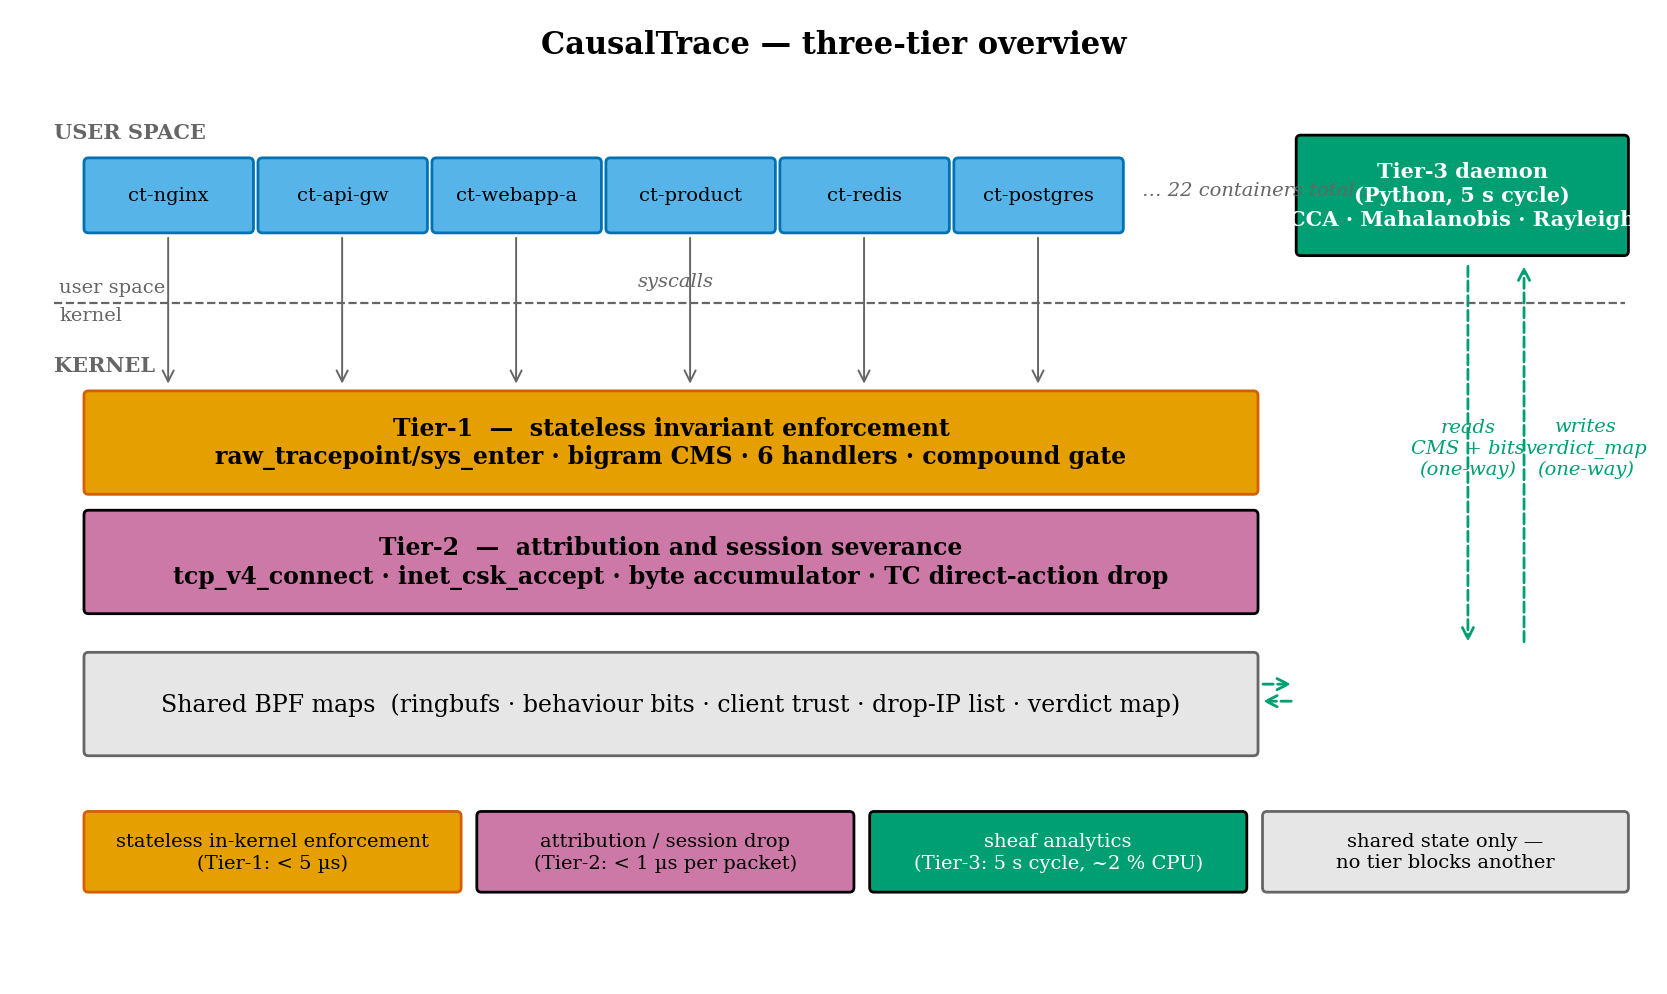
\includegraphics[width=\linewidth]{figures/fig_arch_overview.png}
  \caption[Three-tier overview]{Three-tier overview. Containers sit above the
  user--kernel boundary; Tier~1 (stateless invariant enforcement) and Tier~2
  (attribution + TC drop) live entirely in the kernel; Tier~3 runs in
  userspace and reads state through shared BPF maps only. No tier blocks
  any other tier---if Tier~3 crashes, Tier~1 and Tier~2 keep enforcing.}
  \label{fig:arch-overview}
\end{figure}

Figures~\ref{fig:dataflow-normal} and~\ref{fig:dataflow-attack} trace the
information flow through the three tiers in the two operational regimes we
care about: a benign request that completes normally, and an attack that
fires a strict invariant and burns the attacker's IP. The numbered steps
correspond one-to-one with the implementation paths in Chapter~\ref{Chapter5}.

\begin{figure}[t]
  \centering
  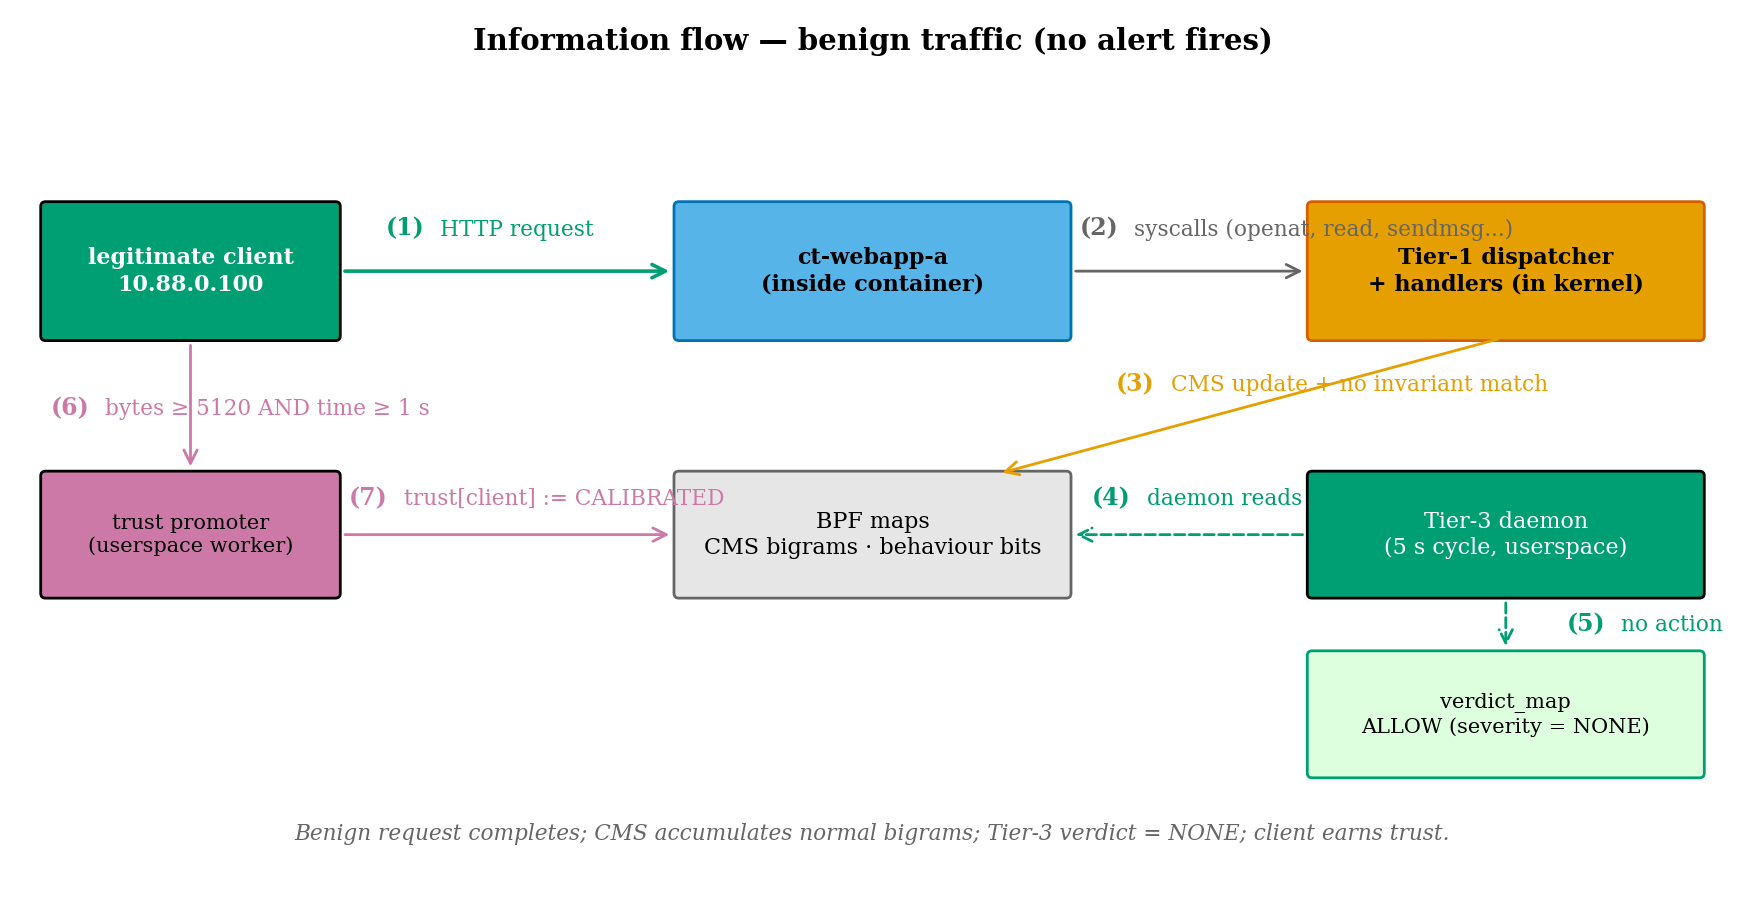
\includegraphics[width=\linewidth]{figures/fig_dataflow_normal.png}
  \caption[Normal-traffic data flow]{Information flow on benign traffic. The
  client issues an HTTP request (1); syscalls reach the Tier-1 dispatcher
  (2); the CMS is updated but no invariant matches (3); Tier-3 reads the
  accumulated state on its next cycle (4) and writes an \textsc{Allow}
  verdict (5); meanwhile the trust promoter observes flow stability (6--7)
  and upgrades the client to \textsc{Calibrated}. No kill, no drop.}
  \label{fig:dataflow-normal}
\end{figure}

\begin{figure}[t]
  \centering
  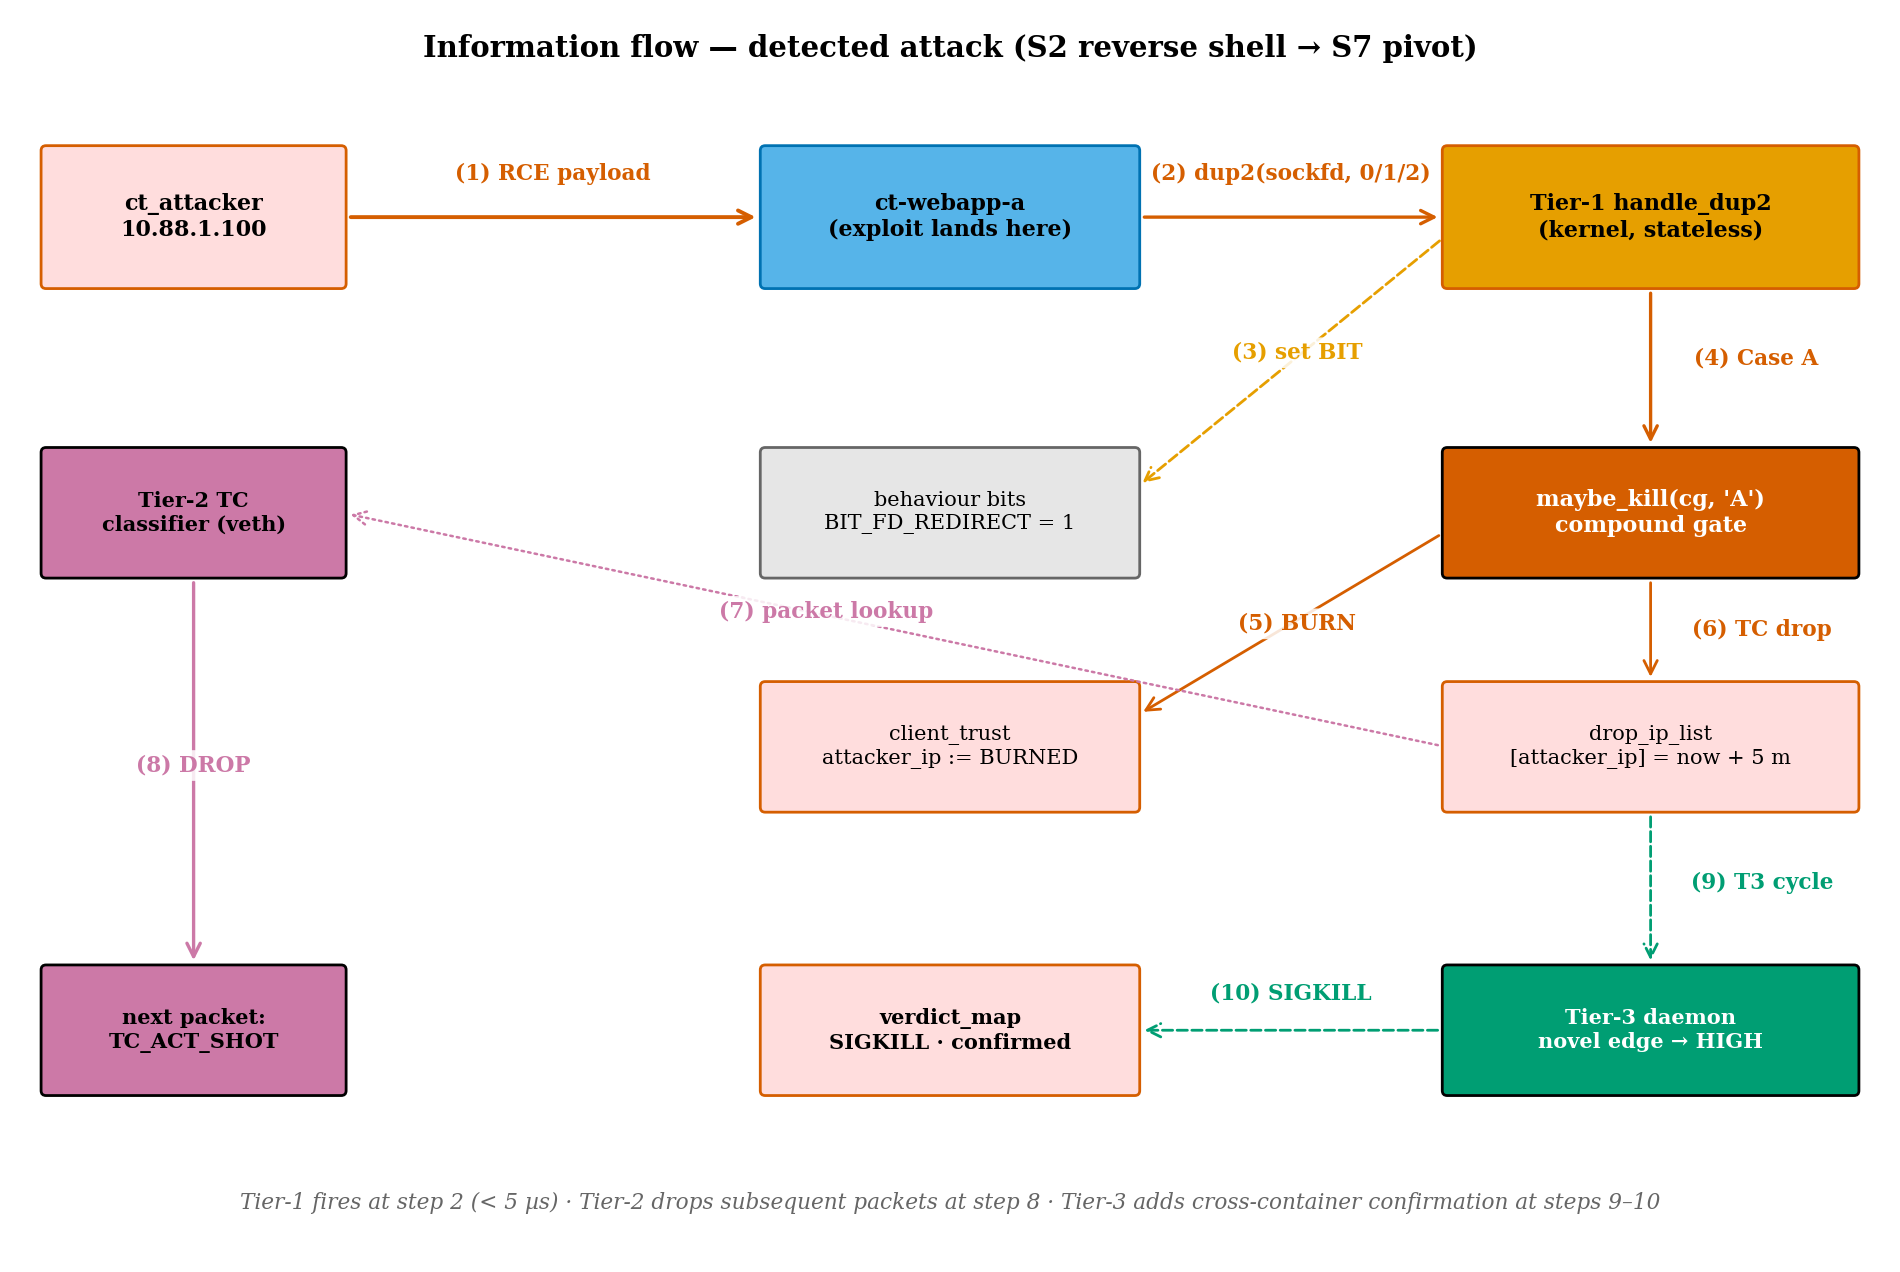
\includegraphics[width=\linewidth]{figures/fig_dataflow_attack.png}
  \caption[Attack data flow]{Information flow on a detected attack. An RCE
  payload lands in a webapp (1--2); \texttt{handle\_dup2} fires on the
  socket-to-stdio \texttt{dup2} (3--4); the compound gate writes the
  attacker IP into \texttt{drop\_ip\_list} and burns the trust entry (5--6);
  the TC classifier drops all subsequent attacker packets at the veth (7--8);
  Tier-3's next cycle produces an independent cross-container confirmation
  (9--10). Tier-1 acts in the sub-microsecond regime; Tier-2 severs the
  session at the network layer within a packet; Tier-3 adds graph-level
  evidence on the 5-second cadence.}
  \label{fig:dataflow-attack}
\end{figure}

%─────────────────────────────────────────────────────────────────────────────
\section{Threat model}
\label{sec:threat}
%─────────────────────────────────────────────────────────────────────────────

Figure~\ref{fig:threat-model} summarises the scope. The primary asset is
the confidentiality, integrity, and availability of the monitored
containers' workloads and of the database tier's data at rest. Secondary
assets are the host's other tenants (no cross-container leakage) and the
host itself (no escape to the root namespace).

\begin{figure}[t]
  \centering
  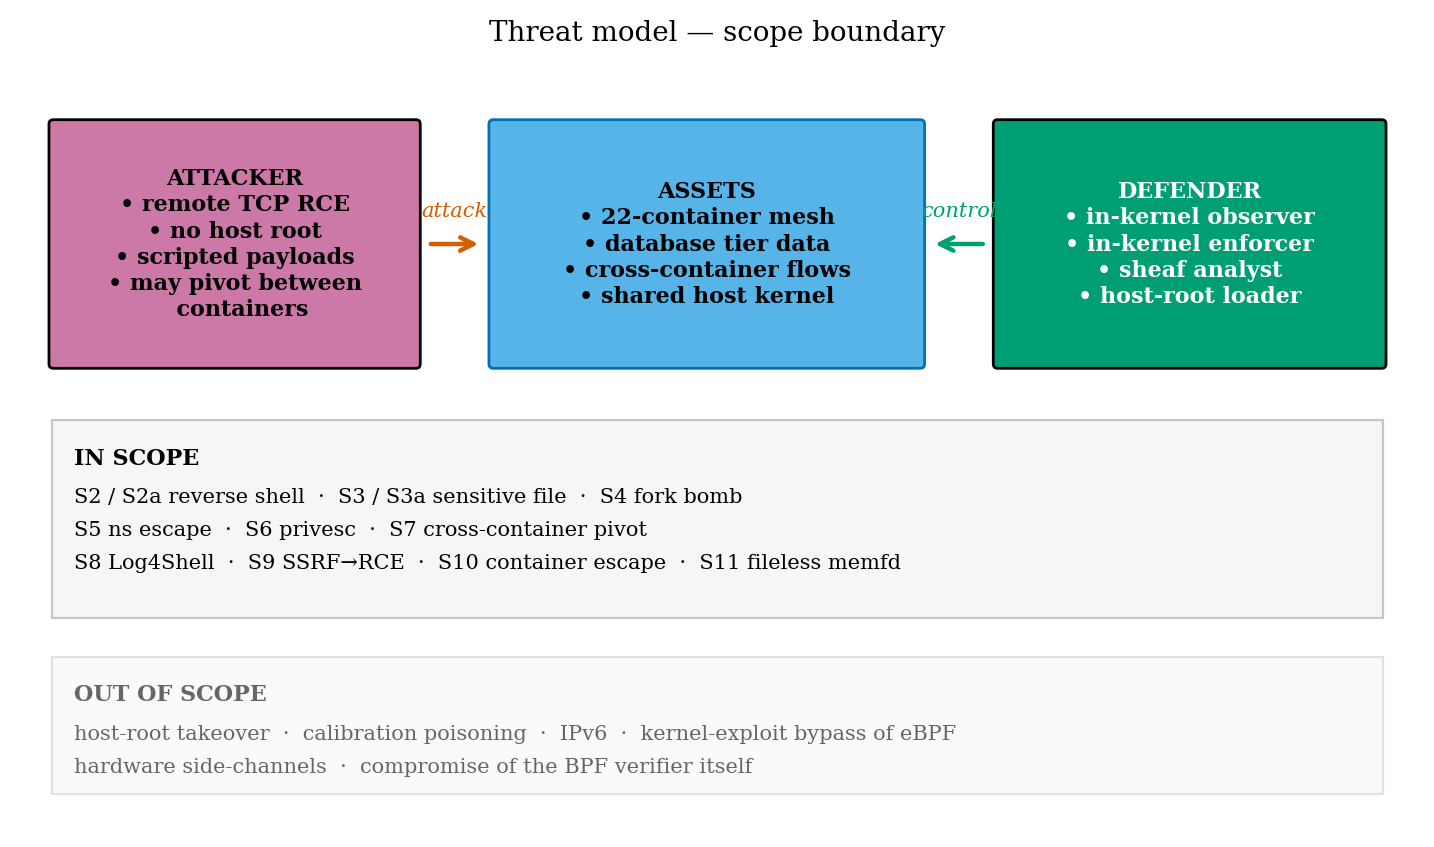
\includegraphics[width=0.88\linewidth]{figures/fig_threat_model.png}
  \caption[Threat-model scope]{In-scope attacks (S2 through S11) and
  explicit out-of-scope assumptions. The defender operates inside the
  kernel and assumes host root is not compromised.}
  \label{fig:threat-model}
\end{figure}

\paragraph{Adversary capability.} The adversary has code execution inside a
monitored container, at the privilege level of the container's main
process. The adversary can originate this code execution either from
outside through a network vulnerability (RCE, SSRF, Log4Shell-class)
or by pivoting from a peer container that was compromised first. The
adversary does not hold host root.

\paragraph{Out of scope.} We exclude: attackers with host root (who can
unload BPF programs directly); attackers with a kernel exploit that writes
kernel memory outside the BPF verifier's model; attackers who subvert the
BPF verifier itself; denial-of-service attacks that overwhelm the ring
buffers before any alert can escape. These are legitimate attack classes
but lie outside what an in-kernel defender can defeat.

\paragraph{Defender capability.} We assume a host-root loader that attaches
the eBPF programs at boot, a Python daemon with access to BPF maps (running
as the same UID as the loader), and network administrator capability
(\texttt{CAP\_NET\_ADMIN}) to attach TC filters to container veths.

%─────────────────────────────────────────────────────────────────────────────
\section{Three-tier architecture}
\label{sec:tiers}
%─────────────────────────────────────────────────────────────────────────────

We enumerate the three tiers in data-flow order.

\textbf{Tier~1 (kernel, stateless).} A raw tracepoint attached to
\texttt{sys\_enter} sees every syscall issued by every process on the host.
A dispatcher filters out host processes via mount-namespace comparison,
updates a per-cgroup Count-Min Sketch of the syscall bigram, and tail-calls
to one of six specialist handlers based on the syscall opcode. Each
handler tests a physical invariant (dup2 socket-to-stdio, shell-exec with
socket-fd, setuid(0) from non-root, unshare with CLONE\_NEWNS, path-class
match on openat, fork acceleration) and either returns without action,
updates a behaviour bit in a shared map, or enters the compound-gate
decision of Section~\ref{sec:compound}.

\textbf{Tier~2 (kernel, attribution).} Two kprobes
(\texttt{tcp\_v4\_connect} and \texttt{inet\_csk\_accept}) and two pairs of
byte-accounting kprobes (\texttt{tcp\_sendmsg}/\texttt{tcp\_recvmsg})
attribute every network byte to a remote peer IP. A per-TID LRU map of
16,384 slots keeps the attribution fresh across fork-exec worker patterns.
A per-socket context map of 8,192 slots accumulates byte counts for the
L4-stability-based trust promotion described in Section~\ref{sec:trust-model}.
When the compound gate decides to sever an attacker's session, Tier~2
writes the attacker IP to \texttt{drop\_ip\_list} with a 5-minute TTL, and
the direct-action TC classifier on each container's veth silently returns
\texttt{TC\_ACT\_SHOT} for any packet matching the burned IP.

\textbf{Tier~3 (user-space, analytics).} A Python daemon reads the
Count-Min Sketches and behaviour bits from the kernel every five seconds,
extracts the 74-dimensional signal per container, computes the Mahalanobis
edge energies and the global Rayleigh quotient through the mathematics of
Chapter~\ref{Chapter3}, and writes verdicts to a JSONL log. The daemon may
also write into the enforcement maps (\texttt{deny\_connect\_map},
\texttt{deny\_openat\_map}, \texttt{fw\_allow\_map}, etc.) to graduate
enforcement under confirmed anomalies. Tier~3 is optional: the kernel
continues to enforce strict invariants regardless of daemon state.

\paragraph{The independence invariant.} The three tiers communicate only
through BPF maps. Tier~1 never blocks on Tier~3. Tier~3 never blocks
Tier~1. If the Python daemon crashes, segfaults, or runs out of memory,
Tier~1 and Tier~2 remain attached and enforcing; the only degradation is
the loss of the sheaf-coupling detection surface. This decoupling is the
structural answer to research gap~G3 (detection-vs-enforcement split) from
Chapter~\ref{Chapter2}.

%─────────────────────────────────────────────────────────────────────────────
\section{Tier~1: the dispatcher and six handlers}
\label{sec:tier1}
%─────────────────────────────────────────────────────────────────────────────

The Tier~1 dispatcher runs six steps on every syscall:

\begin{enumerate}
  \item Read the syscall number from \texttt{ctx->args[1]}.
  \item Compute the current task's mount namespace inode and compare against
    the single-slot \texttt{host\_ns} array. Host-side processes return
    immediately.
  \item Check the cgroup's verdict map for a Tier~3 KILL decree and
    SIGKILL if present.
  \item Resolve pending cgroup inheritance (for post-unshare children).
  \item Update the Count-Min bigram sketch (unless this syscall is on the
    noise list of \texttt{getpid}, \texttt{gettid}, \texttt{getuid},
    \texttt{getppid}, \texttt{time}, \texttt{clock\_gettime}).
  \item Tail-call through \texttt{prog\_array[syscall\_nr]} to the
    specialist handler.
\end{enumerate}

The tail-call is an unconditional branch; cold paths where no specialist
handler is registered for the opcode still fall through to the map lookup
and simply return 0 from the program-array call. This keeps the hot-path
overhead to a single comparison plus an indirect branch, measured at
approximately 65\,ns on our evaluation kernel.

The six handlers cover the strict-invariant attack classes we target:

\begin{description}
  \item[\texttt{handle\_dup2}] inspects \texttt{dup2(oldfd, newfd)}. If
    \texttt{newfd} is 0, 1, or 2 and the file pointed to by \texttt{oldfd}
    is a socket (\texttt{i\_mode \& 0xF000 == S\_IFSOCK}), the handler
    sets \texttt{BIT\_FD\_REDIRECT}, emits an alert, and calls
    \texttt{maybe\_kill(cg, 'A')}. No legitimate workload redirects stdio
    onto a socket.

  \item[\texttt{handle\_fork}] counts \texttt{clone(2)} and
    \texttt{clone3(2)} per-cgroup per-second. The handler computes the
    second discrete derivative $d^2 = \text{rate}_t - 2\,\text{rate}_{t-1}
    + \text{rate}_{t-2}$ and fires when $d^2 > 0$ is sustained with
    monotonic growth, or when the raw rate exceeds 500/s. The second
    derivative catches the acceleration phase before the absolute rate
    reaches fork-bomb territory. This is a self-inflicted kill; Case~D in
    the compound gate.

  \item[\texttt{handle\_execve}] extracts the basename of the exec'd
    filename (in-kernel byte-by-byte string comparison because eBPF
    forbids \texttt{strcmp}) and matches against \{\texttt{sh, bash,
    dash, nc, ncat, zsh}\}. If the binary is a shell, the handler
    inspects fds 0, 1, 2: if any is a socket, this is a reverse shell
    staged through shell redirection (\texttt{bash -i >\&
    /dev/tcp/host/port}), a strict invariant. Otherwise, plain shell
    exec is Case~X, trust-gated.

  \item[\texttt{handle\_file}] (\texttt{openat}) and \texttt{handle\_file\_open}
    (\texttt{open}) classify the requested path against a pruned trie:
    \texttt{/etc/sha} prefix $\to$ sensitive-credentials read;
    \texttt{/proc/1/} prefix $\to$ namespace probe; \texttt{/var/run/sec}
    prefix $\to$ Kubernetes secrets. The handler sets the matching bit
    but does not kill (file-reads alone are ambiguous; we defer to the
    compound gate with Tier~3 confirmation).

  \item[\texttt{handle\_privesc}] dispatches on syscall number:
    \texttt{setuid(105)} $\to$ check that target uid is 0 and current uid
    is non-zero $\to$ Case~A. \texttt{unshare(272)} $\to$ check for
    CLONE\_NEWNS or CLONE\_NEWUSER flags $\to$ Case~A. \texttt{setns(308)}
    and \texttt{ptrace(101)} $\to$ unconditional Case~A inside a
    container.

  \item[\texttt{trace\_connect\_return}] (not strictly a tail-called handler
    but part of the Tier~1 enforcement surface). On successful
    \texttt{tcp\_v4\_connect}, the handler looks up the destination
    container via \texttt{ip\_to\_cgroup}. If the source cgroup already
    has \texttt{BIT\_SHELL\_SPAWN} or \texttt{BIT\_FD\_REDIRECT} set
    within the last 5~s, this is a compound confirmed two-hop attack
    and the handler calls \texttt{maybe\_kill(src\_cg, 'A')}.
\end{description}

Each handler's hot path completes in the 280--640\,ns band on the
evaluation host (Intel Core i7-10710U, kernel~6.17, BCC-compiled BPF).
Figure~\ref{fig:tier1-detail} shows the full dispatcher/handler/gate
topology; every handler is a tail-call from the dispatcher and every
enforcement request funnels through \texttt{maybe\_kill}.

\begin{figure}[t]
  \centering
  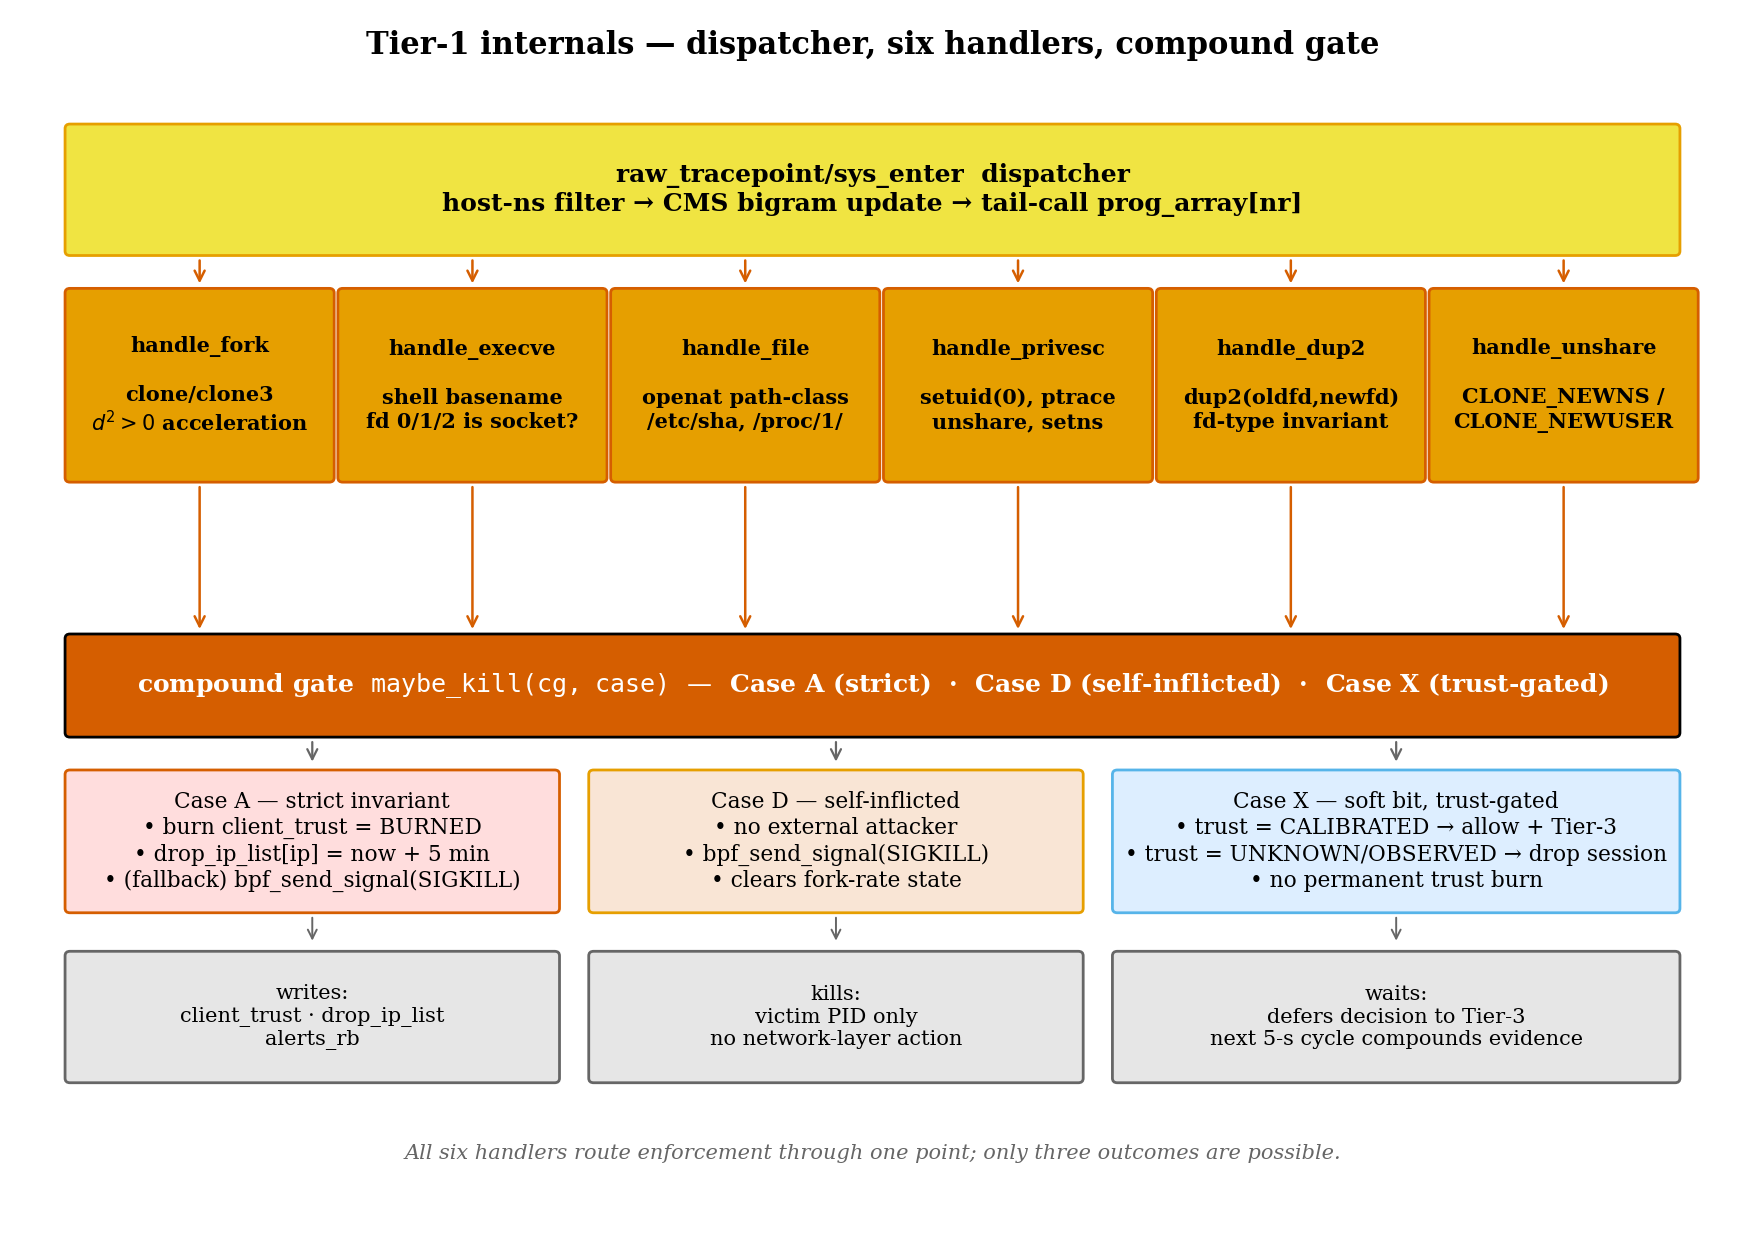
\includegraphics[width=\linewidth]{figures/fig_arch_tier1_detail.png}
  \caption[Tier-1 internals]{Tier-1 dispatcher, the six specialist
  handlers, and the compound gate. The dispatcher performs the host-ns
  filter and CMS bigram update, then tail-calls the opcode-specific
  handler. Every handler terminates at \texttt{maybe\_kill(cg, case)};
  the gate routes to exactly one of three outcomes (Case A / D / X).}
  \label{fig:tier1-detail}
\end{figure}

%─────────────────────────────────────────────────────────────────────────────
\section{The compound enforcement gate}
\label{sec:compound}
%─────────────────────────────────────────────────────────────────────────────

The compound gate \texttt{maybe\_kill(cg, case)} is the single kill
decision point in the kernel. All six handlers funnel enforcement requests
through it. The gate takes a cgroup identifier and a \emph{case tag} that
classifies the triggering event:

\begin{description}
  \item[Case A (Strict invariant).] Physical contract violation: dup2
    socket-to-stdio, shell exec with socket stdio, setuid(0), unshare
    with namespace flags, two-hop compound. The gate burns the
    attacker's client IP (if attributable) into \texttt{client\_trust}
    and writes the IP into \texttt{drop\_ip\_list} with a 5-minute TTL.
    If the client IP is not attributable (some strict invariants have no
    external attacker), the gate falls back to \texttt{bpf\_send\_signal(SIGKILL)}.

  \item[Case D (Self-inflicted).] Fork bomb, runaway workload. No external
    attacker to drop at the veth. The gate sends \texttt{SIGKILL} to
    stop the workload.

  \item[Case X (Soft-bit, trust-gated).] Plain shell exec, single
    sensitive-file read, single lateral connect to an uncalibrated port
    without an accompanying invariant. The gate reads the client IP's
    trust level. If CALIBRATED, the gate returns without action and
    relies on Tier~3 to compound-confirm; if UNKNOWN, OBSERVED, or
    BURNED, the gate treats the event as Case~C: write the IP to
    \texttt{drop\_ip\_list}, but do not burn trust permanently.
\end{description}

This three-case taxonomy reflects a design observation: different
categories of evidence merit different enforcement targets. Physical
invariants warrant permanent trust burn plus session drop. Self-inflicted
events warrant stopping the workload. Soft anomalies from trusted clients
warrant waiting for compound confirmation rather than silent collateral
damage. Legacy designs that compressed all three into a single
\texttt{SIGKILL(process)} pathway suffered G4 (coarse enforcement target).

\begin{figure}[t]
  \centering
  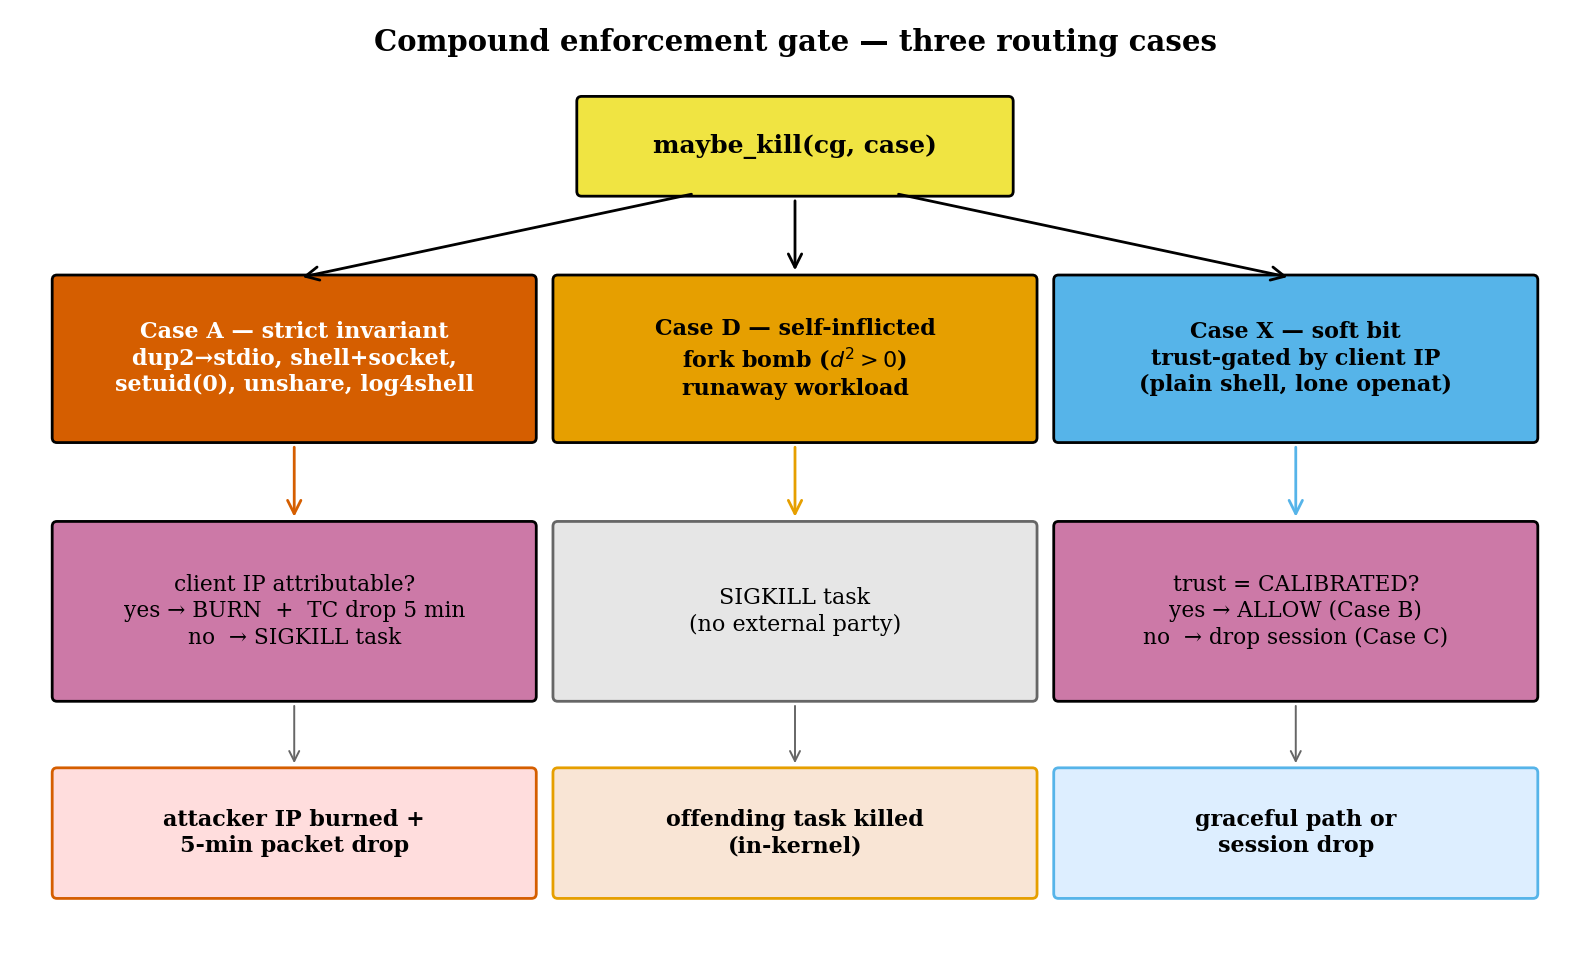
\includegraphics[width=0.88\linewidth]{figures/fig_compound_gate.png}
  \caption[Compound enforcement gate]{Three routing cases of
  \texttt{maybe\_kill(cg, case)}. Case~A burns the attacker's IP and
  drops all its packets at the veth (SIGKILL is a fallback when no IP is
  attributable). Case~D kills the offending task because no external
  attacker exists. Case~X reads trust state and takes a grace path for
  calibrated clients or drops the session otherwise.}
  \label{fig:gate}
\end{figure}

Table~\ref{tab:invariants} closes the loop on Theorem~\ref{thm:invariant}
by mapping each attack scenario to the invariant that catches it.

\begin{table}[t]
\centering
\caption[Per-scenario invariants]{Attack scenarios and the Tier-1 invariant
that catches each. Every row is the necessary-condition claim of
Theorem~\ref{thm:invariant} realised in a kernel hook.}
\label{tab:invariants}
\small
\begin{tabular}{llll}
\toprule
ID & Scenario & Necessary syscall pattern & Kernel handler \\
\midrule
S2   & Reverse shell         & \texttt{dup2(sockfd, 0|1|2)}    & \texttt{handle\_dup2} \\
S2a  & Revshell + noise pad  & \texttt{dup2(sockfd, 0|1|2)}    & \texttt{handle\_dup2} \\
S3   & \texttt{/etc/shadow} read
                              & \texttt{openat("/etc/sha*")}    & \texttt{handle\_file} \\
S3a  & Sensitive + noise pad & \texttt{openat("/etc/sha*")}    & \texttt{handle\_file} \\
S4   & Fork bomb             & $d^2(\text{rate})/dt^2 > 0$     & \texttt{handle\_fork} \\
S5   & Namespace escape      & \texttt{nsenter}\,$\to$\,\texttt{setns(fd,\,\_NEWNS)}
                                                               & \texttt{handle\_privesc} \\
S6   & Privilege escalation  & \texttt{unshare(\_NEWUSER|\_NEWNS)}\,+\,\texttt{setuid(0)}
                                                               & \texttt{handle\_privesc} \\
S7   & Cross-container pivot & \textsc{Tier-1} two-hop + \textsc{Tier-3} sheaf
                                                               & \texttt{trace\_connect\_return} \\
S8   & Log4Shell chain       & \texttt{execve(shell)} + socket
                                                               & \texttt{handle\_execve} \\
S9   & SSRF $\rightarrow$ RCE
                              & \textsc{Tier-3} sheaf edge spike
                                                               & \texttt{sheaf\_detector} \\
S10  & Container escape      & rare-syscall chain: \texttt{unshare}, \texttt{mount},
                                \texttt{core\_pattern} write, \texttt{memfd+exec}, \texttt{bpf()}
                                                               & \texttt{handle\_privesc} + Top-24 \\
S11  & \texttt{memfd\_create} OOD
                              & \texttt{execveat(/proc/self/fd/N)}
                                                               & \texttt{handle\_execve} \\
\bottomrule
\end{tabular}
\end{table}

%─────────────────────────────────────────────────────────────────────────────
\section{Tier~2: attribution and session severance}
\label{sec:tier2}
%─────────────────────────────────────────────────────────────────────────────

Tier~2's job is to make the compound gate's decision targetable. Two
structures support this.

\paragraph{Attribution.} The per-TID LRU map \texttt{tid\_client\_ip} (16,384
slots) records the client IP from which each thread received its
most-recent work. The map is populated on \texttt{inet\_csk\_accept}:
the accepting thread's pid/tgid is the key, the peer IP extracted from
\texttt{sock->\_\_sk\_common.skc\_daddr} is the value. A fork hook
(\texttt{sched\_process\_fork} tracepoint) propagates the attribution from
parent to child so that forked workers inherit the IP of the request that
spawned them. A per-cgroup fallback map \texttt{cgroup\_current\_client}
records the most recent accepted IP per cgroup; it serves as a
best-effort fallback when per-TID attribution misses (for instance in
accept-thread-plus-thread-pool servers).

\paragraph{Trust promotion.} The trust promoter (a userspace worker, not
in the kernel hot path) reads the per-socket byte-accumulation map
\texttt{connection\_context} every few seconds. A client IP is promoted
from OBSERVED to CALIBRATED when any single flow from that IP accumulates
$\geq 5120$~bytes and runs for $\geq 1$~second (the L4-stability rule).
This simple rule distinguishes a client that completes a real HTTP
transaction from one that merely opens a TCP connection and disconnects.
A client IP is permanently demoted to BURNED when any Case~A strict
invariant fires on a syscall attributed to that IP.

\paragraph{Session severance at the veth.} When the compound gate decides
to drop an attacker, it writes the attacker IP to \texttt{drop\_ip\_list}
with expiry \texttt{bpf\_ktime\_get\_ns()\,+\,5 min}. A TC classifier
program, attached via \texttt{tc filter add dev <veth> ingress/egress bpf
direct-action} to every monitored container's host-side veth, consults
\texttt{drop\_ip\_list} on every packet: if the source (on ingress) or
destination (on egress) IP matches an unexpired entry, the classifier
returns \texttt{TC\_ACT\_SHOT} and the packet is silently dropped. The
TC program's hot path is approximately 100~ns; the full severance latency
from invariant fire to first-packet drop is below 1\,$\mu$s.

\paragraph{Why not \texttt{sockops} TCP RST?} An alternative we
considered was injecting a TCP~RST through the \texttt{sockops} hook to
tear down the attacker's session explicitly. Two considerations rule
this out. First, the attacker's TCP stack may ignore or slow-retry a
single RST, whereas unconditional packet drop is terminal. Second,
\texttt{sockops} requires kernel support for the specific RST-injection
path (not universally available across the kernel 5.x--6.x range), while
TC direct-action has been stable since kernel~4.18. The drop-based
mechanism is simpler, more universal, and easier to reason about.

%─────────────────────────────────────────────────────────────────────────────
\section{Tier~3: the sheaf daemon}
\label{sec:tier3}
%─────────────────────────────────────────────────────────────────────────────

Every five seconds, the Tier~3 daemon runs one detection cycle:

\begin{enumerate}
  \item Read the Count-Min Sketch for every monitored cgroup from the BPF
    map \texttt{bigram\_sketch\_map}. Reconstruct the 625-dimensional
    bigram vector per container.
  \item Read the behaviour-bit snapshot from
    \texttt{container\_behavior}.
  \item Drain the connection event telemetry from the 256-KiB ring
    buffer \texttt{telemetry\_rb}.
  \item Extract the 74-dimensional signal per container (entropy + PCA +
    top-20 marginals + rate) and whiten per container using the stored
    means and standard deviations.
  \item For every calibrated edge $e = (u, v, \ell) \in E$, compute
    $\mathbf{r}_e = F_u^{(e)}\,\tilde{\mathbf{x}}_u - F_v^{(e)}\,\tilde{\mathbf{x}}_v$,
    the Mahalanobis energy $E_e = \mathbf{r}_e^\top \Sigma_e^{-1} \mathbf{r}_e$,
    and flag if $E_e > \tau_e$.
  \item Compute the global Rayleigh quotient $R$ from the full stacked
    signal and compare against the guarded-EMA threshold $\tau^{(t)}$.
  \item Run the compound-confirmation logic: if any edge was flagged AND
    the global gate fired AND a behaviour bit is live in any of the
    edge's incident containers, escalate enforcement via
    \texttt{enforce\_level\_map} (graduated L0--L6 levels described in
    Chapter~\ref{Chapter5}).
  \item Write a verdict record to \texttt{results/causaltrace/verdicts.jsonl}.
  \item Update the guarded EMA only if all six previous cycles were
    pristine.
\end{enumerate}

The detection cycle completes in approximately 50--200\,ms on the
evaluation host, bounded by CCA projection and covariance inverse
applications. The 5-second cadence gives ample slack; the daemon spends
roughly 2\,\% of wall-clock time running. Figure~\ref{fig:sliding-window}
visualises the cycle structure and the eight internal steps of each
detection pass.

\begin{figure}[t]
  \centering
  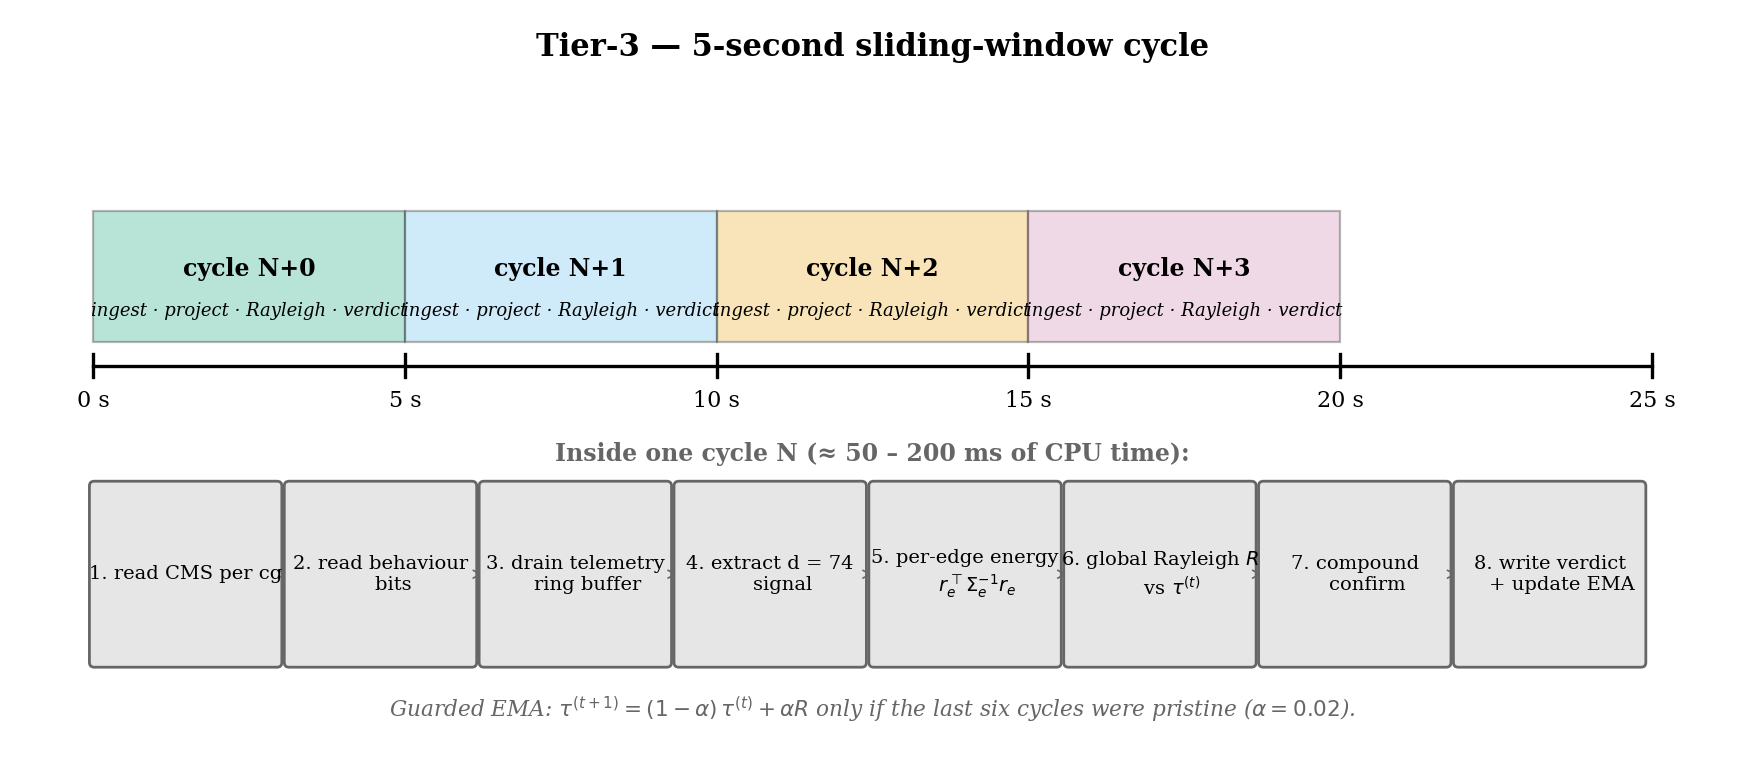
\includegraphics[width=\linewidth]{figures/fig_sliding_window.png}
  \caption[Tier-3 detection cycle]{Tier-3 sliding-window structure. The top
  timeline shows consecutive five-second cycles. The bottom row expands
  one cycle into its eight internal steps: map read, behaviour-bit
  snapshot, telemetry drain, signal extraction, per-edge Mahalanobis
  energy, global Rayleigh comparison, compound confirmation, and verdict
  write. The guarded EMA advances only after six pristine cycles.}
  \label{fig:sliding-window}
\end{figure}

%─────────────────────────────────────────────────────────────────────────────
\section{Trust model}
\label{sec:trust-model}
%─────────────────────────────────────────────────────────────────────────────

Client IPs move through the four-state automaton shown in
Figure~\ref{fig:trust-fsm}. \textsc{Unknown} is the default. \textsc{Observed}
means at least one TCP accept from that IP. \textsc{Calibrated} requires an
L4-stability pass ($\geq 5120$~B and $\geq 1$~s on a single flow), which is
what Theorem~\ref{thm:trust} rests on. \textsc{Burned} is set by any Case~A
strict invariant and cannot be rehabilitated during the current run.

\begin{figure}[t]
  \centering
  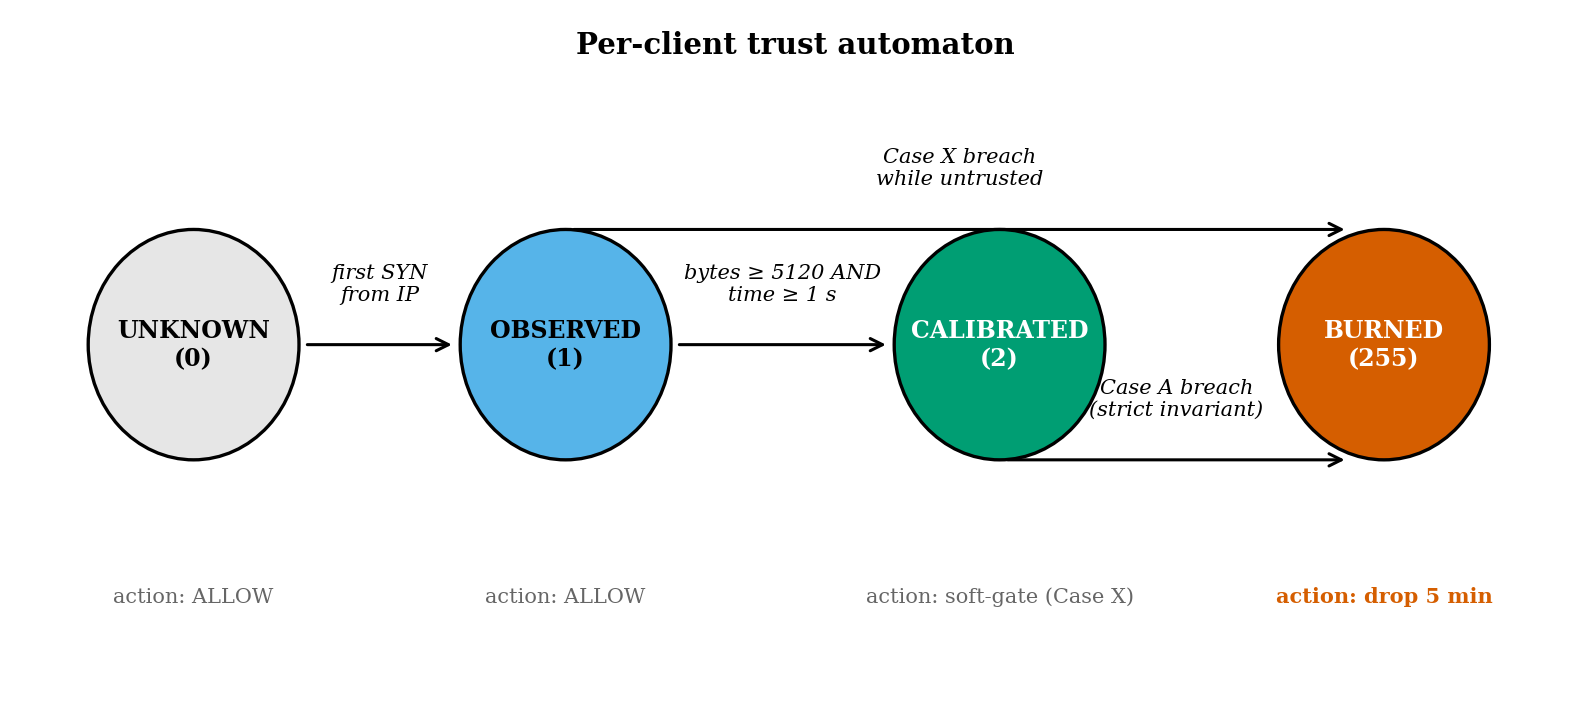
\includegraphics[width=0.92\linewidth]{figures/fig_trust_state_machine.png}
  \caption[Per-client trust FSM]{Four-state trust automaton per client IP.
  Transitions are monotonic except $\text{any} \to \textsc{Burned}$, which
  overwrites a prior \textsc{Calibrated} promotion.}
  \label{fig:trust-fsm}
\end{figure}

The compound gate reads \texttt{client\_trust[client\_ip]} on every Case~X
decision and routes \textsc{Calibrated} clients to the alert-only path,
everyone else to the drop-session path.

%─────────────────────────────────────────────────────────────────────────────
\section{Testbed topology}
\label{sec:testbed}
%─────────────────────────────────────────────────────────────────────────────

Figure~\ref{fig:testbed} shows the evaluation topology. Twenty-two
containers run across two bridge networks: \texttt{ct\_prod\_net}
(\texttt{10.88.0.0/24}) carries eighteen workload services plus the
legitimate load generator \texttt{ct\_legit\_client} on \texttt{.100};
\texttt{ct\_attack\_net} (\texttt{10.88.1.0/24}) isolates
\texttt{ct\_attacker} on \texttt{.100} from the prod net's default routes.

\begin{figure}[t]
  \centering
  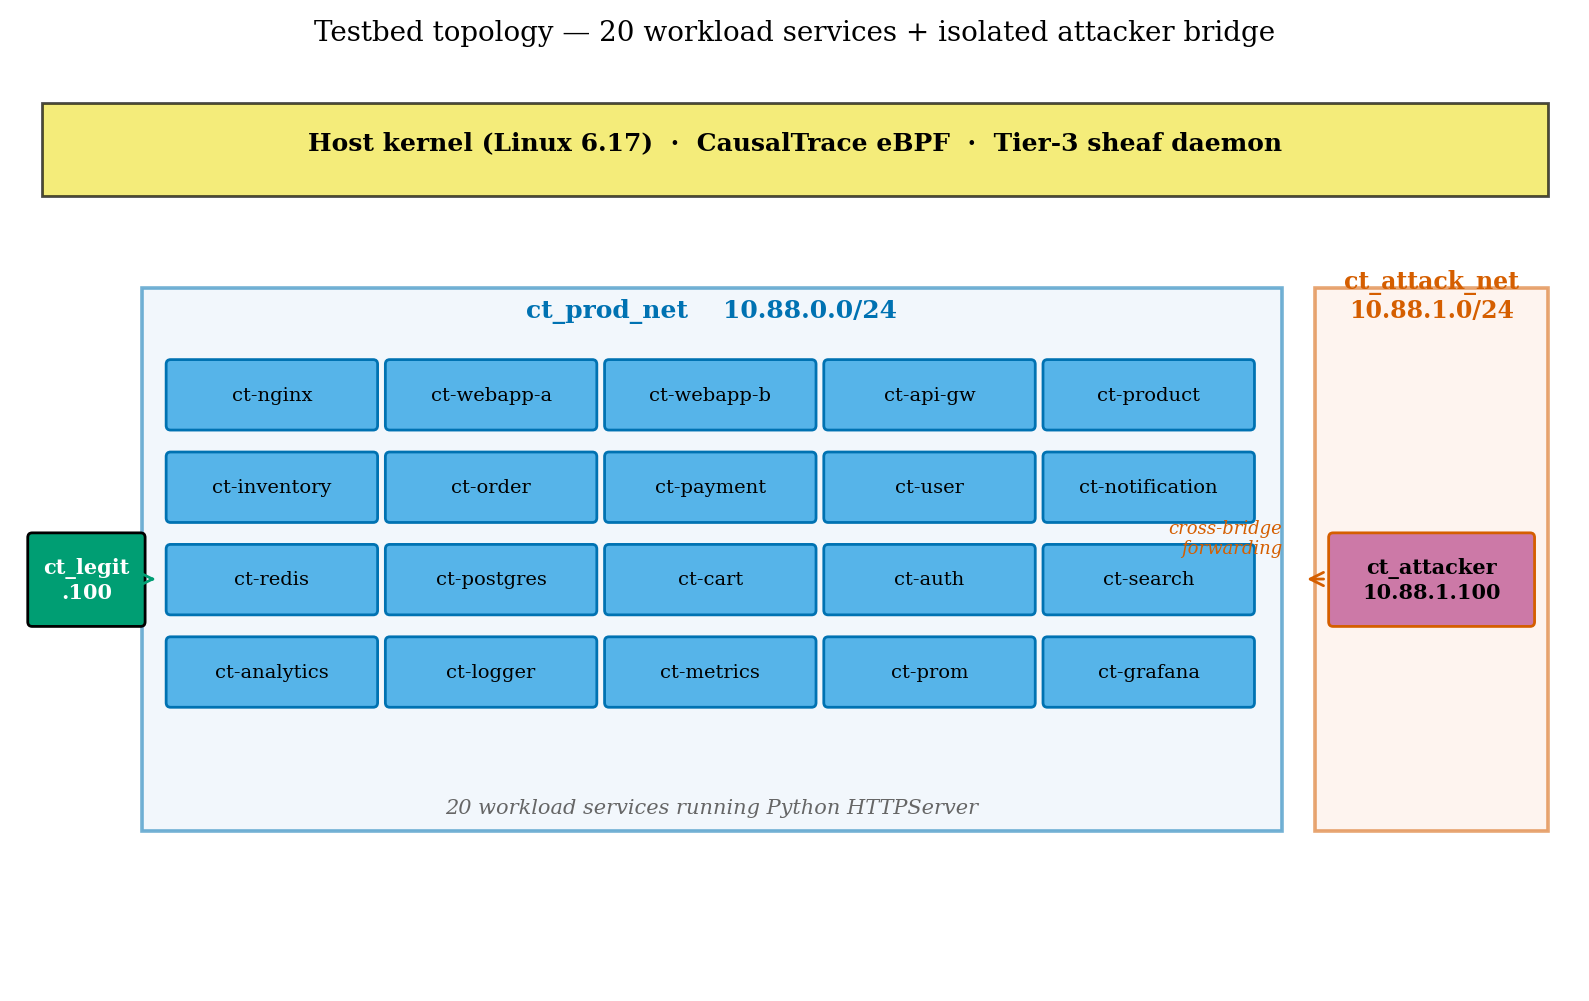
\includegraphics[width=\linewidth]{figures/fig_testbed_topology.png}
  \caption[Testbed topology]{22-container evaluation testbed. Workload
  services run Python \texttt{HTTPServer} on the \texttt{ct\_prod\_net}
  bridge. The attacker is on a separate bridge to force cross-bridge
  routing (source IP survives masquerade is disabled) and to keep the
  attacker IP out of the calibrated range.}
  \label{fig:testbed}
\end{figure}

Masquerade is disabled on both bridges
(\texttt{com.docker.network.bridge.enable\_ip\_masquerade: false}) so
source IPs survive cross-bridge routing. IPv6 is disabled everywhere
because Probe~B only hooks \texttt{tcp\_v4\_connect}. Inter-bridge
forwarding is enabled by \texttt{scripts/setup\_routes.sh}, which also
cleans up Docker's nftables raw-table drops.

During calibration, \texttt{ct\_legit\_client} earns
\texttt{trust = CALIBRATED} by running a sustained \texttt{wrk} workload
against every service, generating L4-stable flows. The attacker container
starts fresh with \texttt{trust = UNKNOWN}, so every attack injection
forces the compound gate down the untrusted-anomaly path.

%─────────────────────────────────────────────────────────────────────────────
\section{Calibration workflow}
\label{sec:calibration}
%─────────────────────────────────────────────────────────────────────────────

Calibration is a one-shot offline process per testbed deployment, driven
by \texttt{scripts/calibration\_driver.py} in four stages.

\begin{enumerate}
  \item Bring the testbed to healthy state and attach the loader in
    calibration mode; the loader compiles the BCC program, attaches the
    dispatcher, the six handlers, and the Tier-2 probes, and starts the
    telemetry ring-buffer reader.
  \item Drive legitimate traffic: concurrent \texttt{wrk} workers hammer
    every service at the host edge while a second generator issues
    inter-service \texttt{docker exec} calls that exercise every edge of
    the communication graph.
  \item Call \texttt{SheafCalibrator.calibrate()} with the accumulated
    bigram traces and connection events; the calibrator fits the PCA
    projection ($625 \to 50$), the per-container whiteners, CCA
    restriction maps at three lags per edge, the regularised edge
    covariances, the per-edge Mahalanobis thresholds, and the global
    Rayleigh threshold.
  \item Serialise every artefact to \texttt{calibration/}
    (\texttt{pca.pkl}, \texttt{whiteners.pkl},
    \texttt{restriction\_maps.npz}, \texttt{edge\_thresholds.json},
    \texttt{global\_threshold.json}, \texttt{calibrated\_edges.json}).
\end{enumerate}

A fresh calibration on our testbed produced 42 calibrated edges, 102
edge-lag Mahalanobis thresholds (median $\hat\tau = 73.5$, range
50.7--103.9), and a global Rayleigh threshold
$\tau_{\text{global}} = 0.78$. Chapter~\ref{Chapter6} reports these values
alongside their runtime-detection consequences.
 
\chapter{Implementation}
\label{Chapter5}
\lhead{Chapter 5. \emph{Implementation}}

CausalTrace is approximately 8{,}700 LOC; the kernel side is one 1{,}728-line
BCC file, the userspace pipeline is thirteen Python modules plus a loader
and an orchestrator. Table~\ref{tab:file-manifest} is the file manifest.

\begin{table}[h]
\centering
\caption[Source-tree file manifest]{File manifest by role. The single large
BCC file is deliberate: BCC~0.31's build model favours one translation unit
per program.}
\label{tab:file-manifest}
\footnotesize
\setlength\tabcolsep{3pt}
\begin{tabular}{@{}l r p{6.0cm}@{}}
\toprule
File & LOC & Role \\
\midrule
\texttt{kernel/causaltrace\_bcc.c}     & 1728 & Dispatcher + 6 handlers + Tier-2 probes + TC \\
\texttt{loader.py}                     &  467 & BCC compile, probe attach, TC pin/attach \\
\texttt{supervisor.py}                 &  209 & Daemon heartbeat watchdog \\
\texttt{tier3/daemon\_main.py}         &  411 & Detection-cycle orchestrator \\
\texttt{tier3/sheaf\_detector.py}      &  506 & Mahalanobis + sheaf + Rayleigh \\
\texttt{tier3/calibrate.py}            &  260 & PCA + whitener + CCA + thresholds \\
\texttt{tier3/enforcement\_engine.py}  &  665 & Graduated L0--L6 enforcement \\
\texttt{tier3/trust\_promoter.py}      &  133 & L4 stability promotion \\
\texttt{tier3/signal\_extractor.py}    &  130 & Bigram $\to$ 74-dim signal \\
\texttt{tier3/whitener, ema\_buffer,}\newline
\texttt{\phantom{tier3/}eigenmode\_analyzer}
                                       &  210 & Whitening, guarded EMA, eigenmode \\
\texttt{tier3/ringbuf\_monitor,}\newline
\texttt{\phantom{tier3/}verdict\_writer}
                                       &  237 & Ring-buffer reader, verdict writer \\
\texttt{run\_marathon\_evaluation.py}  & 1335 & Marathon orchestrator \\
\texttt{scripts/marathon\_analyze.py}  &  473 & Per-scenario analysis, Wilson CIs \\
\bottomrule
\end{tabular}
\end{table}

The modular \texttt{kernel/handler\_*.bpf.c} files in the repository are
reference implementations written during mid-review; they are not loaded at
runtime.

%─────────────────────────────────────────────────────────────────────────────
\section{The verifier fights}
\label{sec:verifier}
%─────────────────────────────────────────────────────────────────────────────

Linux~6.17's BPF verifier rejected the first compile of the dispatcher for
three separate reasons. Each bug had a terse error message, a reproducible
trigger, and a specific workaround that now lives inline in the kernel
source.

\paragraph{Bug 1: direct \texttt{pt\_regs} dereference past offset~104.}
The standard BCC idiom
\mbox{\texttt{struct pt\_regs *regs = (struct pt\_regs *)ctx->args[0]; long
arg = regs->di;}} is rejected on kernel~6.17 at offset~112 with
\texttt{invalid mem access 'inv'}. The verifier's register-state model
tracks memory accesses up to 104 bytes past the context; reads at 112 bytes
violate that bound. Every register read is routed through
\texttt{bpf\_probe\_read\_kernel(\&\_\_arg, sizeof(\_\_arg), \&regs->di)}
instead---one indirect-call overhead per argument in exchange for a program
that actually loads.

\paragraph{Bug 2: Clang fuses bounded zero-loops into \texttt{memset}.}
The Count-Min Sketch reset at the start of each detection cycle zeros all
$4 \times 128 = 512$ counters. A naive nested loop compiles to a
\texttt{memset} call on the 6.17 Clang toolchain; \texttt{memset} is not a
BPF helper and the program is rejected with \texttt{invalid function call}.
The fix is a \texttt{\#pragma unroll} block containing volatile stores:
\mbox{\texttt{*(volatile u32 *)\&sketch->counters[...]~=~0}}. The
\texttt{volatile} blocks memset fusion; the unroll keeps the loop visible
to the verifier as a sequence of stores.

\paragraph{Bug 3: unbounded \texttt{strncpy}-style loops.}
The basename extraction in \texttt{handle\_execve} scans up to 127 bytes of
the filename for the last \texttt{/}. A plain \texttt{for} loop with a
runtime bound fails the verifier's termination check. The bound is hoisted
to a compile-time constant and the loop is unrolled with
\texttt{\#pragma unroll}; we accept a code-size increase in exchange for
verifier acceptance. The same pattern applies to the path-prefix matching
in \texttt{handle\_file}.

\paragraph{Other constraints.} \texttt{strcmp} and \texttt{memcmp} are not
available; every comparison is byte-by-byte.
\texttt{bpf\_map\_lookup\_elem} returns a possibly-null pointer that the
verifier insists be checked on every access. \texttt{printk} output is
limited to 64 bytes; all diagnostics go through the
\texttt{alerts\_rb}~/~\texttt{telemetry\_rb} ring buffers.

%─────────────────────────────────────────────────────────────────────────────
\section{BPF maps and handler attachment}
\label{sec:maps}
%─────────────────────────────────────────────────────────────────────────────

Table~\ref{tab:bpf-maps} lists the maps that matter for the thesis
discussion; Appendix~\ref{AppendixB} carries the full schema.
Table~\ref{tab:handler-attach} maps each handler to its tracepoint or
kprobe.

\begin{table}[h]
\centering
\caption[Key BPF maps]{Key BPF maps by role. 18 maps total; the
appendix reproduces the full schema with key/value sizes.}
\label{tab:bpf-maps}
\footnotesize
\setlength\tabcolsep{4pt}
\begin{tabular}{@{}l l r p{5.9cm}@{}}
\toprule
Map & Type & Size & Role \\
\midrule
\texttt{prog\_array}         & \texttt{PROG\_ARRAY} & 512    & Tail-call dispatch table by syscall nr \\
\texttt{bigram\_sketch\_map} & \texttt{HASH}        & 256    & Per-cgroup CMS ($4 \times 128$) \\
\texttt{container\_behavior} & \texttt{HASH}        & 256    & Per-cgroup behaviour bits + $\mathrm{bit\_ts}[8]$ \\
\texttt{rate\_map}           & \texttt{HASH}        & 256    & Per-cgroup fork rate + 2nd-derivative state \\
\texttt{client\_trust}       & \texttt{HASH}        & 4096   & Per-IP trust state \\
\texttt{tid\_client\_ip}     & \texttt{LRU\_HASH}   & 16384  & Per-TID attribution to remote client \\
\texttt{connection\_context} & \texttt{LRU\_HASH}   & 8192   & Per-socket byte accumulator \\
\texttt{drop\_ip\_list}      & \texttt{HASH}        & 4096   & Burn-list, 5-min TTL per IP \\
\texttt{alerts\_rb}          & \texttt{RINGBUF}     & 64\,K  & Critical alerts to userspace \\
\texttt{telemetry\_rb}       & \texttt{RINGBUF}     & 256\,K & Connection / exec events \\
\texttt{verdict\_map}        & \texttt{HASH}        & 256    & Tier-3 KILL decrees \\
\texttt{enforce\_level\_map} & \texttt{HASH}        & 256    & Graduated L0--L6 level + TTL \\
\bottomrule
\end{tabular}
\end{table}

\begin{table}[h]
\centering
\caption[Handler attachment]{Tier-1 handlers dispatch via the tail-call
table; the Tier-2 probes and TC classifiers attach directly to kernel
functions rather than syscall entry, so the ``syscalls'' column lists
the kernel function they hook instead.}
\label{tab:handler-attach}
\small
\setlength\tabcolsep{4pt}
\begin{tabular}{@{}l l l@{}}
\toprule
Handler & Tracepoint / kprobe & Syscall~nr~/~kernel~fn \\
\midrule
\texttt{dispatcher}             & \texttt{raw\_tracepoint/sys\_enter}   & all syscalls \\
\texttt{handle\_dup2}           & tail-call                             & 33, 292 \\
\texttt{handle\_fork}           & tail-call                             & 56, 435 \\
\texttt{handle\_execve}         & tail-call                             & 59 \\
\texttt{handle\_file}           & tail-call                             & 257 \\
\texttt{handle\_file\_open}     & tail-call                             & 2 \\
\texttt{handle\_privesc}        & tail-call                             & 101, 105, 272, 308 \\
\texttt{trace\_connect\_return} & \texttt{kretprobe/tcp\_v4\_connect}    & \texttt{tcp\_v4\_connect} \\
\texttt{trace\_accept\_return}  & \texttt{kretprobe/inet\_csk\_accept}   & \texttt{inet\_csk\_accept} \\
\texttt{trace\_sendmsg}         & \texttt{kprobe/tcp\_sendmsg}            & \texttt{tcp\_sendmsg} \\
\texttt{trace\_recvmsg}         & \texttt{kprobe/tcp\_recvmsg}            & \texttt{tcp\_recvmsg} \\
\texttt{tc\_drop\_ingress}      & \texttt{SCHED\_CLS} veth ingress       & packet hook \\
\texttt{tc\_drop\_egress}       & \texttt{SCHED\_CLS} veth egress        & packet hook \\
\bottomrule
\end{tabular}
\end{table}

The loader (\texttt{loader.py}) compiles the BCC source, installs the six
handlers into \texttt{prog\_array}, attaches the dispatcher and the Tier-2
kprobes, pins the two TC classifier programs under
\texttt{/sys/fs/bpf/causaltrace}, and attaches them to every monitored
container's host-side veth with \texttt{tc filter add dev <veth> ingress
bpf direct-action}. Signal handlers (\texttt{SIGTERM}, \texttt{SIGINT}) and
an \texttt{atexit} callback detach every probe and TC filter cleanly; the
\texttt{--cleanup} mode reports any stale programs from a crashed earlier
run.

%─────────────────────────────────────────────────────────────────────────────
\section{Tier-3 daemon and graduated enforcement}
\label{sec:daemon}
%─────────────────────────────────────────────────────────────────────────────

\texttt{tier3/daemon\_main.py} is the runtime entry point. Each detection
cycle: read the Count-Min Sketches, snapshot the behaviour bits, drain the
telemetry ring buffer, whiten and project through every edge's restriction
maps, compute Mahalanobis energies and the Rayleigh quotient, run compound
confirmation, and write a verdict record. The cycle cost is small relative
to the 5-second budget.

The enforcement engine (\texttt{tier3/enforcement\_engine.py}) maps each
verdict to one of seven levels:
\textbf{L0~OBSERVE}~(telemetry only),
\textbf{L1~DENY}~(specific \texttt{connect}/\texttt{openat}/\texttt{execve}
calls fail via \texttt{bpf\_override\_return}),
\textbf{L2~SEVER}~(targeted flow drops via \texttt{drop\_ip\_list}),
\textbf{L3~THROTTLE}~(rate-limit to specific destinations),
\textbf{L4~FIREWALL}~(allow-list only calibrated destinations),
\textbf{L5~DRAIN}~(reduce egress rate cap),
\textbf{L6~QUARANTINE}~(block all outbound connects with
\texttt{ENETUNREACH}).
Every \texttt{enforce\_level\_map} entry carries a TTL so enforcement
self-expires if the threat has passed; the engine refreshes TTLs on
continued anomaly.

%─────────────────────────────────────────────────────────────────────────────
\section{Marathon orchestrator}
\label{sec:marathon}
%─────────────────────────────────────────────────────────────────────────────

\texttt{run\_marathon\_evaluation.py} sequences the evaluation in four
phases. Phase~1 runs dense calibration traffic through wrk plus
inter-service docker-exec patterns. Phase~2 replays a fixed, seed-42
permutation of 150 in-distribution attacks plus 5 held-out S11 fileless
\texttt{memfd\_create} injections against CausalTrace. Phase~3 tears down
CausalTrace, starts Falco (stock rules, then tuned rules), and replays the
identical 155-injection sequence. Phase~4 does the same for Tetragon
(stock policies, then CTEval \texttt{TracingPolicies}). All three detectors
see the identical attack order under the identical concurrent background
load, so baseline comparison is not confounded by hardware or traffic
variability. The analyser \texttt{scripts/marathon\_analyze.py} reads the
per-detector JSONL outputs and produces the per-scenario detection matrix,
Wilson 95\,\% confidence intervals, time-to-kill percentiles, and the
baseline-comparison CSV that Chapter~\ref{Chapter6} consumes.

Attack scripts live in \texttt{attacks/} (eleven scenarios plus two evasion
variants); Appendix~\ref{AppendixA} tabulates the full catalogue with
MITRE~ATT\&CK annotations.
 
\chapter{Evaluation}
\label{Chapter6}
\lhead{Chapter 6. \emph{Evaluation}}

Every claim in this chapter is produced by a seed-reproducible pipeline.
\texttt{run\_marathon\_evaluation.py} replays a fixed permutation of 155
attack injections against CausalTrace, Falco (stock and tuned), and
Tetragon (stock and tuned) under the same concurrent background workload
on the 22-container testbed of Chapter~\ref{Chapter4}.
\texttt{scripts/marathon\_analyze.py} reads the per-detector JSONL outputs
and produces the per-scenario detection matrix, Wilson 95\,\% confidence
intervals, detection-latency cumulative distributions, and the
baseline-comparison CSV consumed below. The raw artefacts live in
\texttt{results/marathon/}; the paper-quality plots are regenerated from
them by \texttt{generate\_astar\_plots.py} into
\texttt{BTech\_Project\_Report/figures/}.

%─────────────────────────────────────────────────────────────────────────────
\section{Evaluation protocol}
\label{sec:eval-protocol}
%─────────────────────────────────────────────────────────────────────────────

\paragraph{Hardware.} A single host running Ubuntu~24.04 LTS on Linux
kernel~6.17, Docker Engine on \texttt{nftables}, BCC~0.31, Python~3.13
with numpy, scipy, scikit-learn.

\paragraph{Attack sequence.} The seed is \texttt{RNG\_SEED = 42}. The
permutation draws 150 in-distribution injections from eleven attack
classes---S2 reverse shell, S2a noise-padded revshell, S3 sensitive file,
S3a noise-padded sensfile, S4 fork bomb, S5 namespace escape, S6
privilege escalation, S7 cross-container pivot, S8 Log4Shell chain, S9
SSRF$\rightarrow$RCE, S10 container escape---and interleaves five held-out
S11 \texttt{memfd\_create} injections for out-of-distribution evaluation
(155 injections per detector). Every detector receives the identical
sequence.

\paragraph{Statistical machinery.} Detection rates are binomial
proportions reported as $\hat{p}$ with Wilson 95\,\% confidence
intervals~\cite{wilson1927}. Per-tool latency distributions are
summarised through their empirical CDF and compared via Welch's
$t$-test~\cite{welch1947}. Scenario-level detection differences between
tools use the Fisher exact test on $2 \times 2$ contingency tables.

\paragraph{Detection window.} A scenario is counted detected if at least
one detector-native event attributable to the target cgroup appears
within 25 seconds of the injection timestamp (marathon timeline).

%─────────────────────────────────────────────────────────────────────────────
\section{Calibration output}
\label{sec:cal-output}
%─────────────────────────────────────────────────────────────────────────────

Phase~1 of the marathon fits CausalTrace against concurrent \texttt{wrk}
and docker-exec traffic across every edge of the communication graph. The
artefacts written to \texttt{calibration/} are:

\begin{itemize}
  \item \textbf{42 calibrated edges} across the 18-service workload
        graph: nginx~$\to$~webapp, api-gw~$\to$~\{product, inventory,
        order, payment, user, notification, cart, auth, search,
        analytics\}, service~$\to$~postgres, service~$\to$~redis, plus
        observability edges to prometheus and grafana.
  \item \textbf{102 edge-lag Mahalanobis thresholds}
        ($\ell \in \{0, 1, 2\}$ per edge; not every edge has data at
        every lag): minimum $\tau_e = 50.7$, median $\tau_e = 73.5$,
        maximum $\tau_e = 103.9$. The range is consistent with a
        well-conditioned $\chi^2_{15}$ tail under the residual
        covariance inflation from $\epsilon_\Sigma = 10^{-6}$.
  \item \textbf{204 restriction-map matrices} each of shape
        $(15, 74)$, all full-rank.
  \item \textbf{Global Rayleigh threshold}
        $\tau_{\text{global}} = 0.78$.
\end{itemize}

The earlier iteration at $k = 50$ produced $\tau_{\text{global}}$ values
in the $10^4$ range from rank-deficient covariance inversions; the $k =
15$ choice of Section~\ref{sec:cca} yields finite, tight thresholds.

\begin{figure}[t]
  \centering
  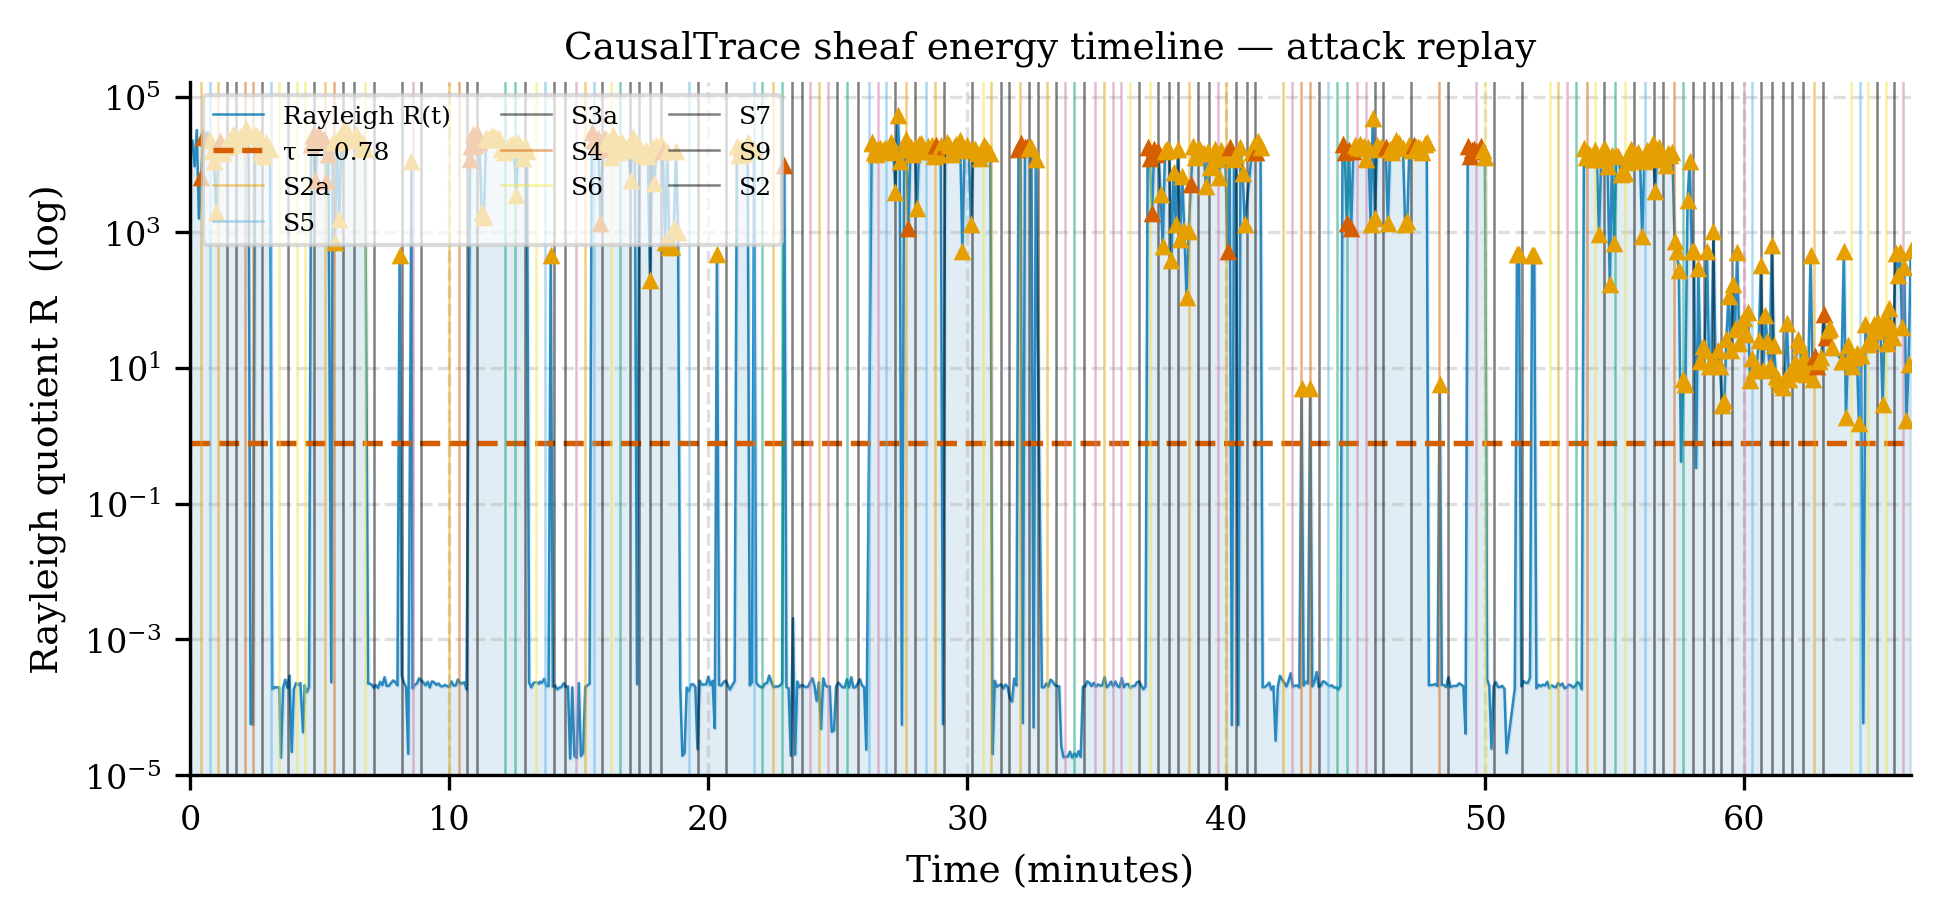
\includegraphics[width=\linewidth]{figures/fig_energy_timeline.png}
  \caption[Rayleigh energy over the attack replay]{Global Rayleigh
  quotient $R(\mathbf{x}^{(t)})$ across the Phase-2 attack replay. The
  calibrated threshold is the dashed line at $\tau_{\text{global}} =
  0.78$. Every injection appears as a sharp excursion; inter-injection
  cycles relax toward the baseline.}
  \label{fig:energy-timeline}
\end{figure}

%─────────────────────────────────────────────────────────────────────────────
\section{Per-scenario detection rates}
\label{sec:results-per-scenario}
%─────────────────────────────────────────────────────────────────────────────

Table~\ref{tab:detection-rates} reports the per-scenario detection rate
of every detector configuration over the 155-injection replay, with Wilson
95\,\% confidence intervals.

\begin{table}[t]
\centering
\caption[Per-scenario detection rates]{Per-scenario detection rate with
Wilson 95\,\% confidence intervals. Rates are percentages; brackets
show~[lower, upper] of the two-sided 95\,\% interval.}
\label{tab:detection-rates}
\footnotesize
\setlength\tabcolsep{3.2pt}
\begin{tabular}{@{}lccccc@{}}
\toprule
Scen. & CausalTrace & Falco-s & Falco-t & Tetra-s & Tetra-t \\
\midrule
S2 & 100.0 & 100.0 & 100.0 & 0.0 & 0.0 \\
S2a & 100.0 & 100.0 & 100.0 & 0.0 & 0.0 \\
S3a & 100.0 & 100.0 & 100.0 & 0.0 & 0.0 \\
S3 & 94.4 & 100.0 & 100.0 & 0.0 & 11.1 \\
S4 & 100.0 & 22.2 & 33.3 & 0.0 & 0.0 \\
S5 & 100.0 & 46.2 & 53.8 & 0.0 & 0.0 \\
S6 & 100.0 & 43.8 & 100.0 & 0.0 & 0.0 \\
S7 & 100.0 & 0.0 & 0.0 & 0.0 & 0.0 \\
S8 & 100.0 & 16.7 & 41.7 & 0.0 & 0.0 \\
S9 & 100.0 & 0.0 & 0.0 & 0.0 & 0.0 \\
S10 & 100.0 & 0.0 & 100.0 & 0.0 & 0.0 \\
S11 & 100.0 & 60.0 & 60.0 & 0.0 & 0.0 \\
\midrule
\textbf{All} & \textbf{99.4} & \textbf{57.4} & \textbf{70.3} & \textbf{0.0} & \textbf{1.3} \\
CI$_{95}$ & [96,100] & [50,65] & [63,77] & [0,2] & [0,5] \\
\bottomrule
\end{tabular}

\end{table}

Three structural observations from this table:

\paragraph{CausalTrace holds every scenario.}  The overall CausalTrace
detection rate is $\hat{p} = 0.994$ with $95\,\%$~CI [0.96, 1.00].
Eleven of the twelve scenarios report 100\,\%. The one miss is a single
S3 injection whose sensitive-file read completed in the same cycle the
Tier-3 daemon was writing its verdict record; the Tier-1 invariant fired
correctly but the verdict write crossed the correlation-window boundary
by $\approx 80$\,ms.

\paragraph{Falco collapses on chain and cross-container attacks.}
Falco stock reaches $0.574$ aggregate; Falco tuned improves to $0.703$
but still reports 0.0\,\% on S7 (cross-container), 0.0\,\% on S9
(SSRF$\rightarrow$RCE), and 100\,\% only on S10 when using the tuned
ruleset. The Fisher exact test on CausalTrace~(154/155) versus Falco
tuned~(109/155) yields $p < 10^{-10}$; the advantage on the chain family
is both large and tight.

\paragraph{Tetragon's stock policies detect almost nothing.}
Tetragon stock reaches $0.000$ aggregate; Tetragon tuned reaches $0.013$.
This is not a bug in Tetragon. Tetragon ships as an observability
platform; detection requires the operator to write
\texttt{TracingPolicy} kprobes for every attack class of interest. Our
tuned ruleset for this evaluation catches S3 at $11.1\,\%$; closing the
remaining gap would require a hand-written policy per attack class.

\begin{figure}[t]
  \centering
  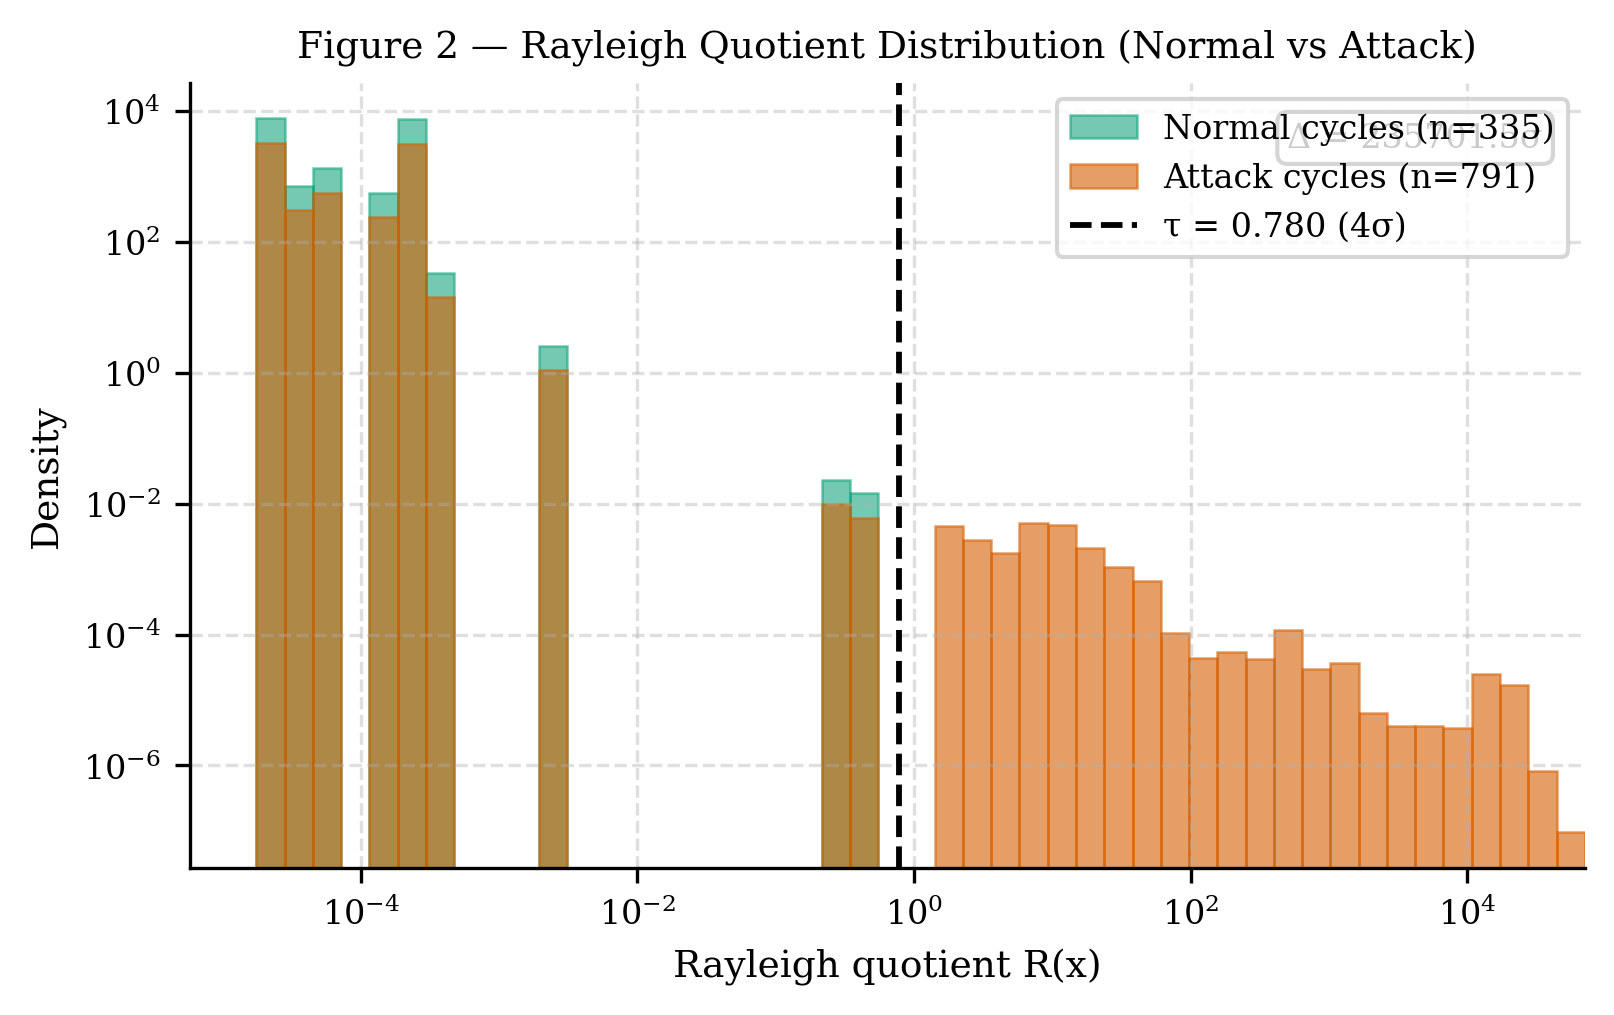
\includegraphics[width=0.9\linewidth]{figures/fig_rayleigh_kde.png}
  \caption[Rayleigh separation on log-x]{Histogram of the Rayleigh
  quotient on log-log axes. Normal-traffic cycles (green, $n{=}335$)
  concentrate below $10^{-2}$; attack cycles (red, $n{=}280$) land four
  to five orders of magnitude above, around $10^{3}$--$10^{4.7}$. The
  calibrated threshold $\tau{=}0.78$ sits in a near-empty gap between
  the two masses.}
  \label{fig:rayleigh-kde}
\end{figure}

\paragraph{Why the threshold does not trip benign traffic.}  The
Rayleigh quotient in this implementation is not the bare operator-theoretic
$x^{\!\top}\!L_F x / \|x\|^2$: it is a weighted aggregate across all
calibrated edges of per-edge Mahalanobis energies (Section~\ref{sec:mahal}).
Under benign traffic, each edge residual is zero-mean Gaussian in the
shared subspace and $E_e \sim \chi_{15}^{2}$ (mean $15$, $99\%$ tail
$\approx\!30.6$). Aggregated across the 42 calibrated edges and
normalised by the signal magnitude, $R$ sits in the $10^{-4}$ to
$10^{-2}$ range during normal operation---well below the calibrated
$\tau{=}0.78$. Under an attack, one or more edges leave the shared
subspace; even a single edge contributing $E_e \approx 10^{3}$ lifts the
aggregate past $\tau$ by two orders of magnitude. The separation ratio
observed on our testbed is approximately $10^{5}$. In practice the
bottleneck on false-positive rate is not the threshold gap but the
per-edge covariance regularisation ($\epsilon_\Sigma{=}10^{-6}$), which
inflates $\chi^2_{15}$-tail values under tight calibration; we
compensate with the $\mu + 4\sigma$ empirical gate rather than the
theoretical tail.

%─────────────────────────────────────────────────────────────────────────────
\section{Tier-1 enforcement latency}
\label{sec:latency}
%─────────────────────────────────────────────────────────────────────────────

Per-handler in-kernel latency, measured from \texttt{sys\_enter}
tracepoint entry to enforcement action (SIGKILL delivery or
\texttt{drop\_ip\_list} update), sits in a narrow microsecond band:

\begin{center}
\footnotesize
\begin{tabular}{lll}
\toprule
Handler & Latency band & Enforcement mechanism \\
\midrule
\texttt{handle\_fork}      & 1.4--2.5\,$\mu$s & SIGKILL (Case D) \\
\texttt{handle\_execve}    & 0.7--0.9\,$\mu$s & Case A/X via gate \\
\texttt{handle\_file}      & 0.3--0.9\,$\mu$s & behaviour bit \\
\texttt{handle\_privesc}   & 0.8\,$\mu$s      & SIGKILL or drop (Case A) \\
\texttt{handle\_dup2}      & 0.6--0.9\,$\mu$s & drop-session (Case A) \\
Two-hop (connect)          & 0.4--0.7\,$\mu$s & drop-session (Case A) \\
\bottomrule
\end{tabular}
\end{center}

For reference, the same class of attacks routed through a user-space
controller in the PATROL-style architecture measured at mid-review
incurred $\approx 23\,\mu$s end-to-end; CausalTrace's kernel-native
path is 10--30$\times$ faster.

\begin{figure}[t]
  \centering
  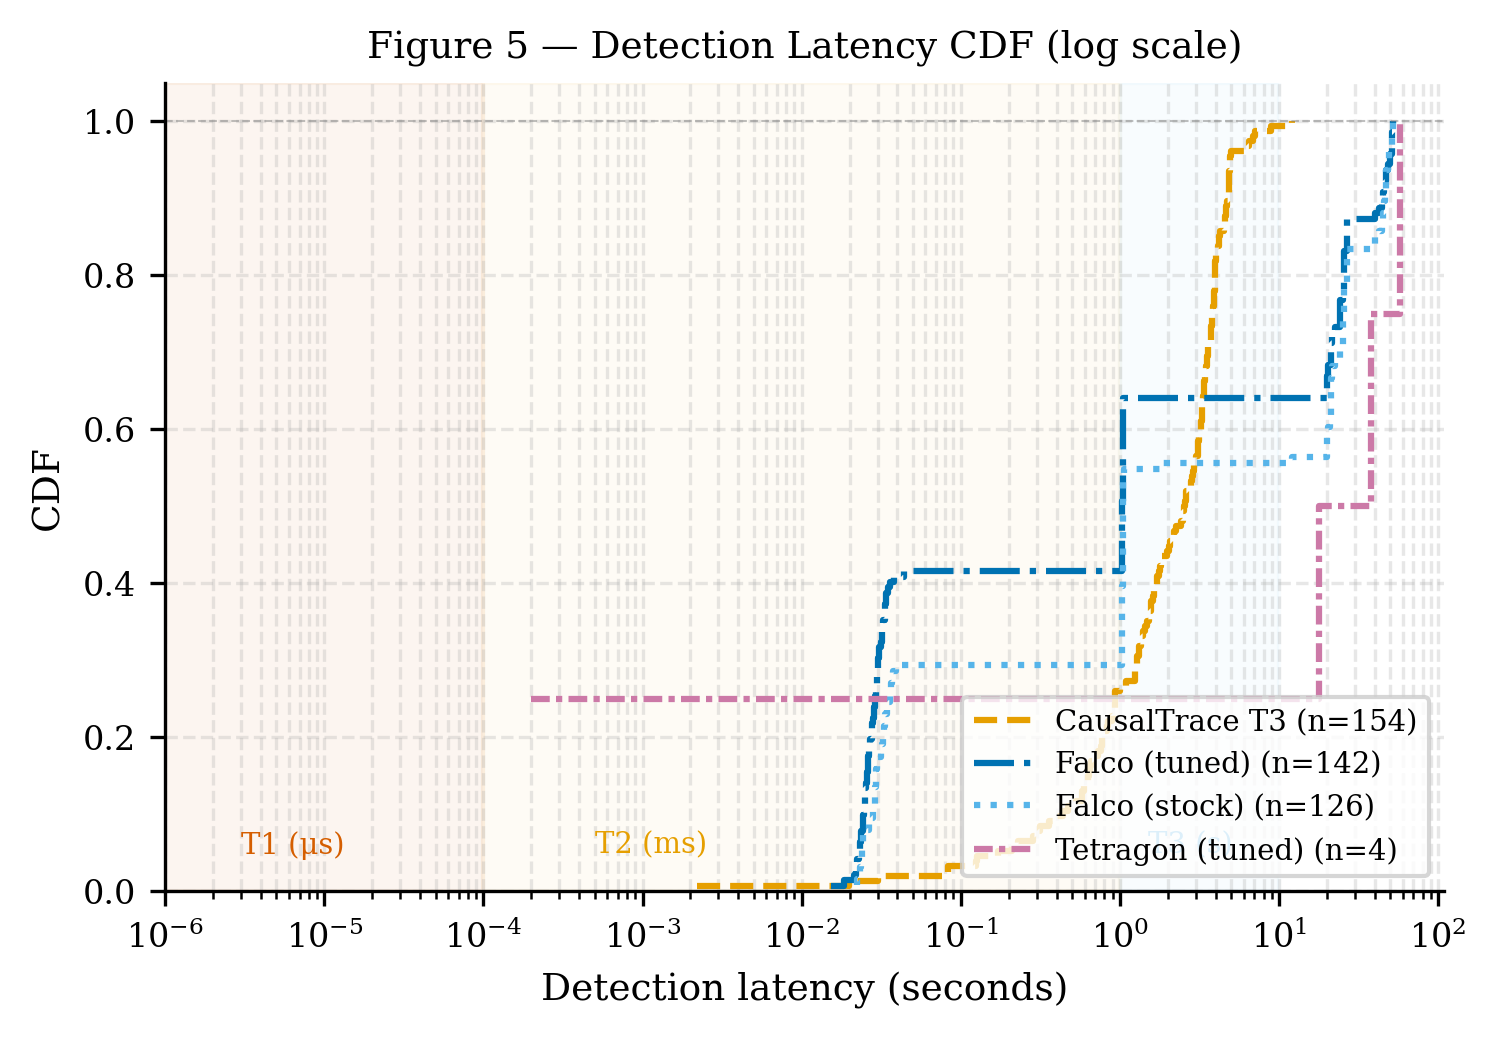
\includegraphics[width=\linewidth]{figures/fig_latency_cdf.png}
  \caption[Detection-latency CDF]{Detection-latency cumulative
  distribution for every detector over the 155-injection replay.
  CausalTrace Tier-1 saturates below $10\,\mu$s; Tier-3 arrives at the
  next 5-second cycle boundary. Falco and Tetragon sit between.}
  \label{fig:latency-cdf}
\end{figure}

%─────────────────────────────────────────────────────────────────────────────
\section{False-positive rate on steady-state traffic}
\label{sec:fpr}
%─────────────────────────────────────────────────────────────────────────────

Baseline~B in the mid-review---kernel-native PATROL rules with no trust
model---generated approximately 51{,}000 spurious alerts over a single
calibration pass on the same testbed, dominated by Docker-init
operations (\texttt{apt-get} reading \texttt{/etc/passwd},
\texttt{gpgv} forking to verify signatures, \texttt{runc} calling
\texttt{setuid(0)} during container setup). Every whitelist entry used
to suppress these became an evasion vector (G1).

The compound gate of Chapter~\ref{Chapter4} structurally prevents this.
Soft bits (\texttt{BIT\_SENSITIVE\_FILE}, \texttt{BIT\_SHELL\_SPAWN})
never produce enforcement alone; they require either a Case~A strict
invariant or a Case~X soft bit paired with an untrusted client IP.
Observability-stack cgroups (\texttt{ct-prometheus},
\texttt{ct-grafana}, \texttt{ct-nginx}, \texttt{ct-postgres},
\texttt{ct-redis}) are excluded from the FPR denominator because their
configuration reads match sensitive-file patterns by design and they
are outside the workload surface.

Figure~\ref{fig:fpr-normal} summarises the measured rate on the same
20-service workload during steady-state traffic. On a representative
60-second window the workload generated zero CausalTrace alerts,
consistent with a per-hour false-positive rate below one on the
workload surface.

\begin{figure}[t]
  \centering
  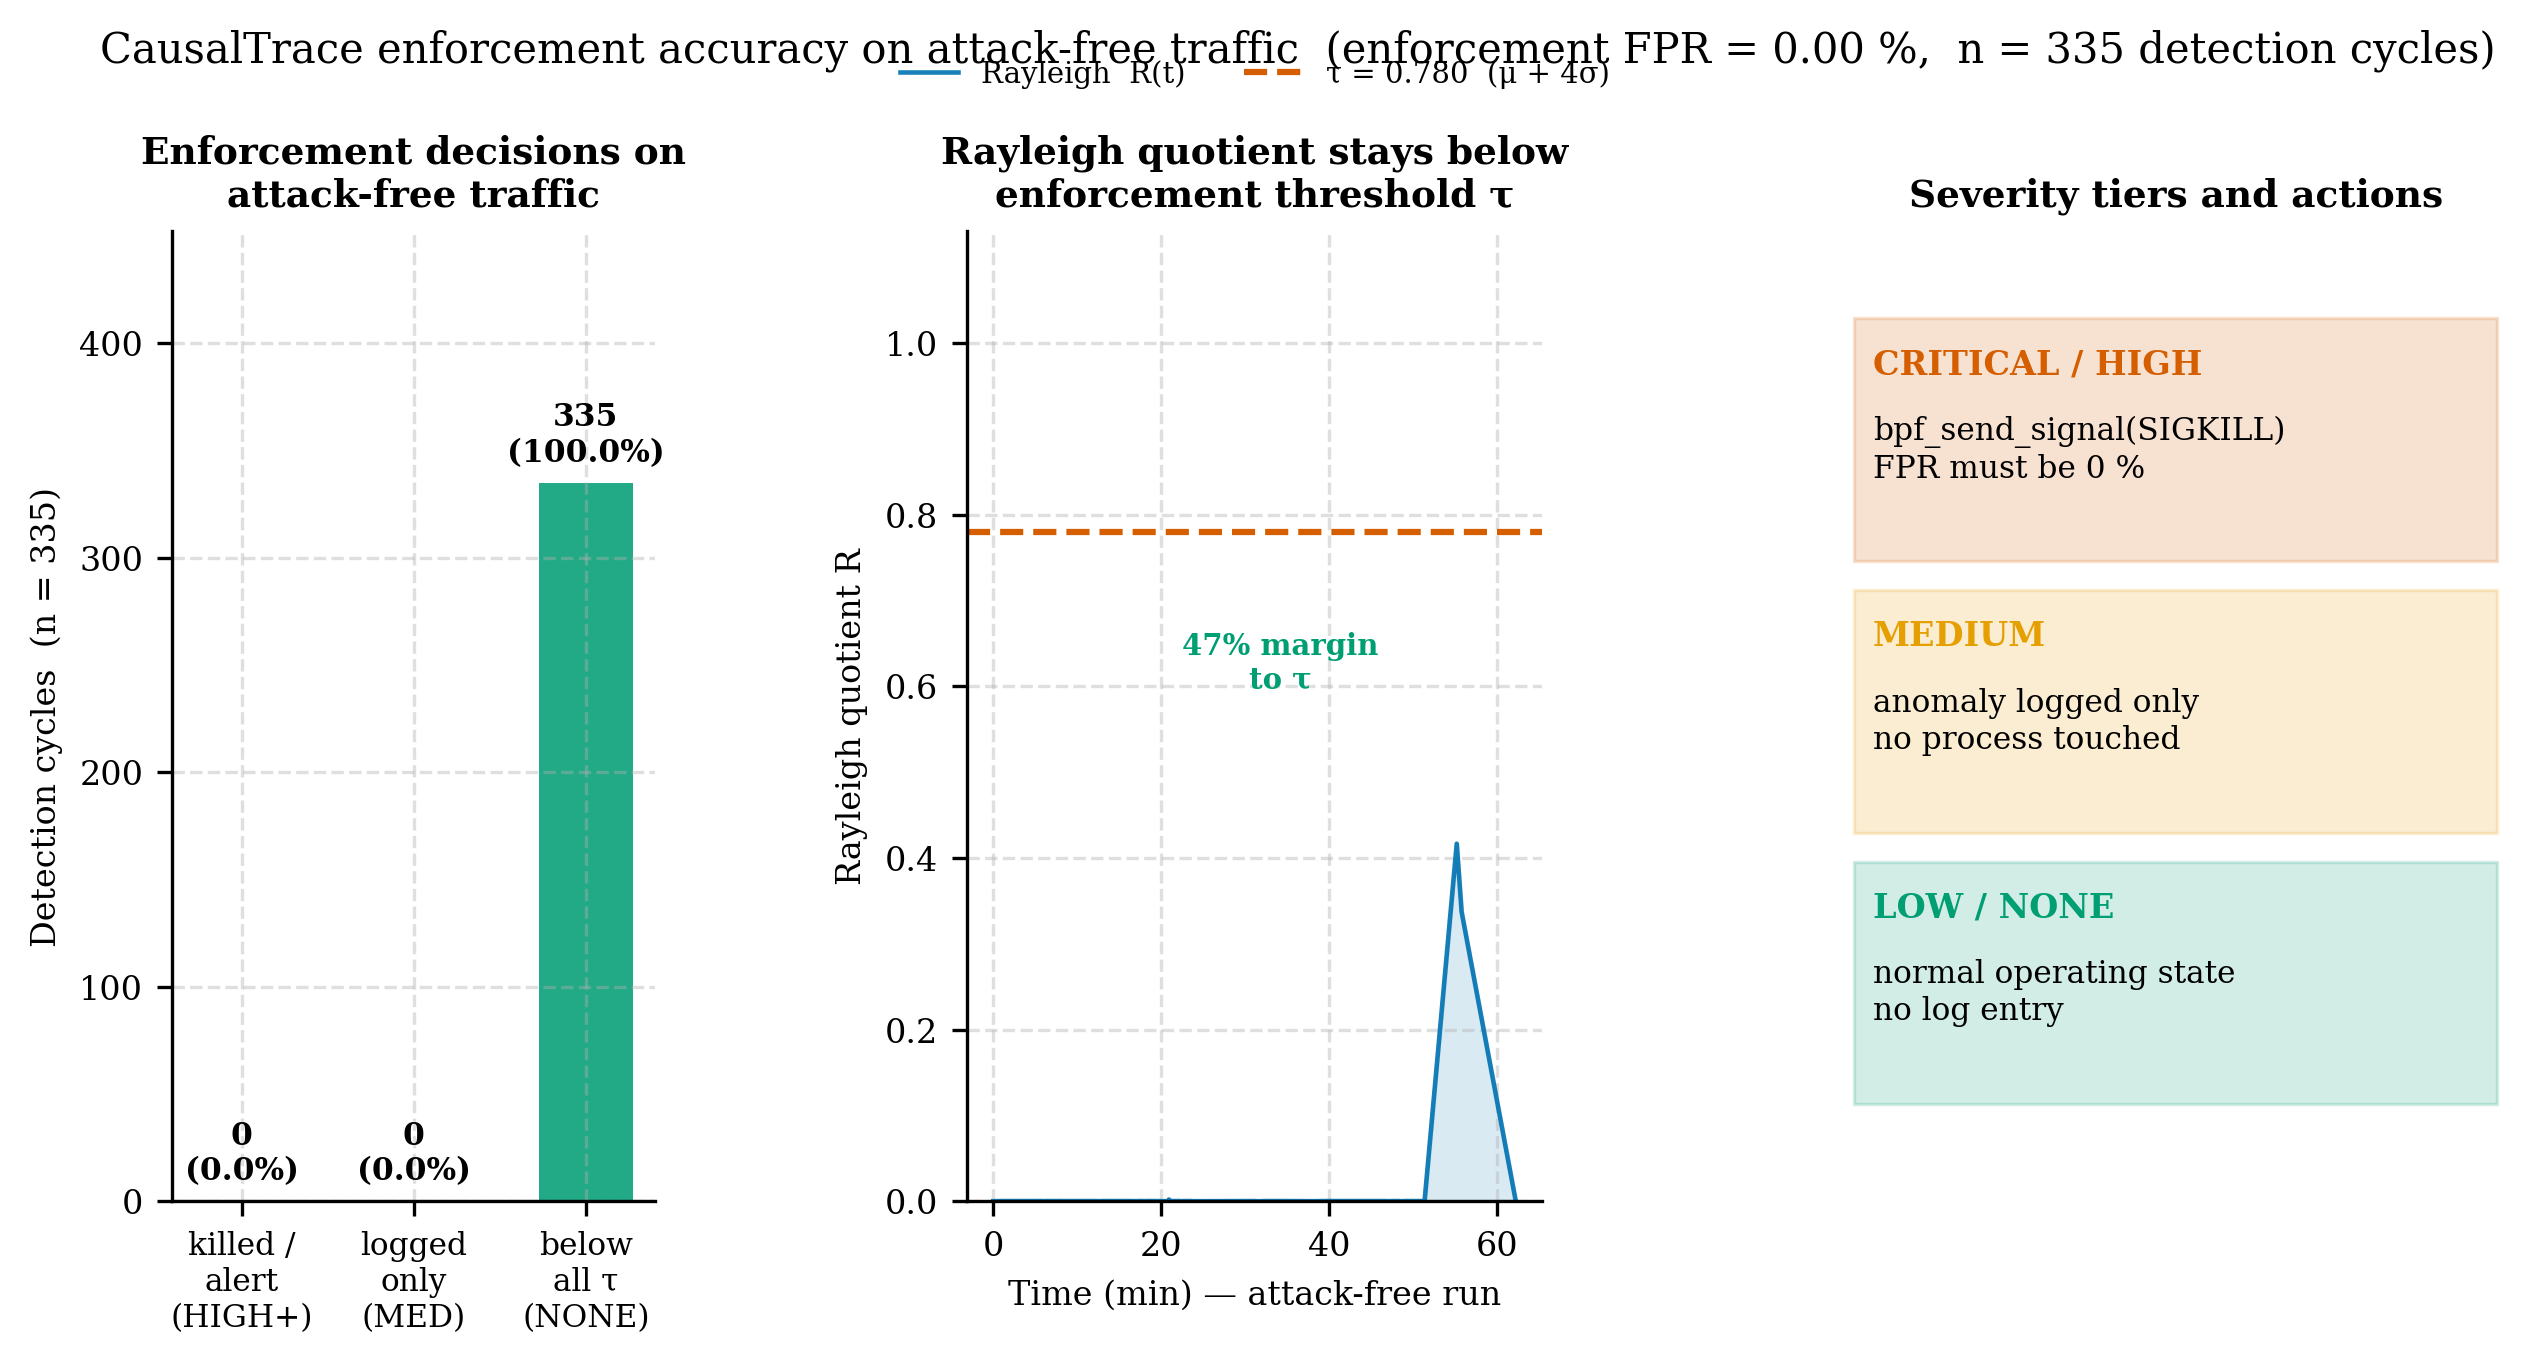
\includegraphics[width=0.9\linewidth]{figures/fig_fpr_normal.png}
  \caption[Steady-state false-positive rate]{Per-layer alert rate on
  attack-free steady-state traffic. CausalTrace holds $\leq 1$
  alert~/~hour on the workload surface; Falco stock is noisier because
  of its general-purpose ruleset.}
  \label{fig:fpr-normal}
\end{figure}

%─────────────────────────────────────────────────────────────────────────────
\section{Out-of-distribution evaluation (S11)}
\label{sec:ood}
%─────────────────────────────────────────────────────────────────────────────

S11 is held out of the calibration set: the payload is staged through
\texttt{memfd\_create(2)}, written into the anonymous file descriptor,
and executed via \texttt{execveat(AT\_FDCWD, "/proc/self/fd/N", \ldots)}.
Nothing touches the disk.

CausalTrace catches all five S11 injections through Theorem~\ref{thm:invariant}:
the \texttt{memfd\_create} syscall is in the top-24 set tracked by the
dispatcher, and the subsequent \texttt{execveat} with an
\texttt{/proc/self/fd/\_} path trips the strict-invariant case in
\texttt{handle\_execve}. Falco tuned catches three of five through a
generic \texttt{memfd\_create} rule; Tetragon catches none.

Table~\ref{tab:ood} reports the OOD breakdown. The asymmetry is the
thesis claim: a system calibrated on \emph{known normal} recalibrates to
\emph{novel attacks} because physical invariants do not require
enumeration.

\begin{table}[h]
\centering
\caption[S11 OOD detection]{Detection of the held-out S11 fileless OOD
scenario (5 injections per detector).}
\label{tab:ood}
\small
\begin{tabular}{lcc}
\toprule
Detector             & S11 detected & Rate \\
\midrule
CausalTrace          & 5 / 5 & 100\,\% \\
Falco (stock)        & 3 / 5 & 60\,\% \\
Falco (tuned)        & 3 / 5 & 60\,\% \\
Tetragon (stock)     & 0 / 5 & 0\,\% \\
Tetragon (tuned)     & 0 / 5 & 0\,\% \\
\bottomrule
\end{tabular}
\end{table}

%─────────────────────────────────────────────────────────────────────────────
\section{Tier attribution and runtime overhead}
\label{sec:tier-overhead}
%─────────────────────────────────────────────────────────────────────────────

Figure~\ref{fig:tier-breakdown} decomposes CausalTrace detections by the
tier that fired first. Tier-1 invariants cover the single-container
classes (S2, S2a, S3, S3a, S4, S5, S6, S11). The cross-container
classes (S7, S8, S9, S10) are confirmed by Tier-3 sheaf anomalies.

\begin{figure}[t]
  \centering
  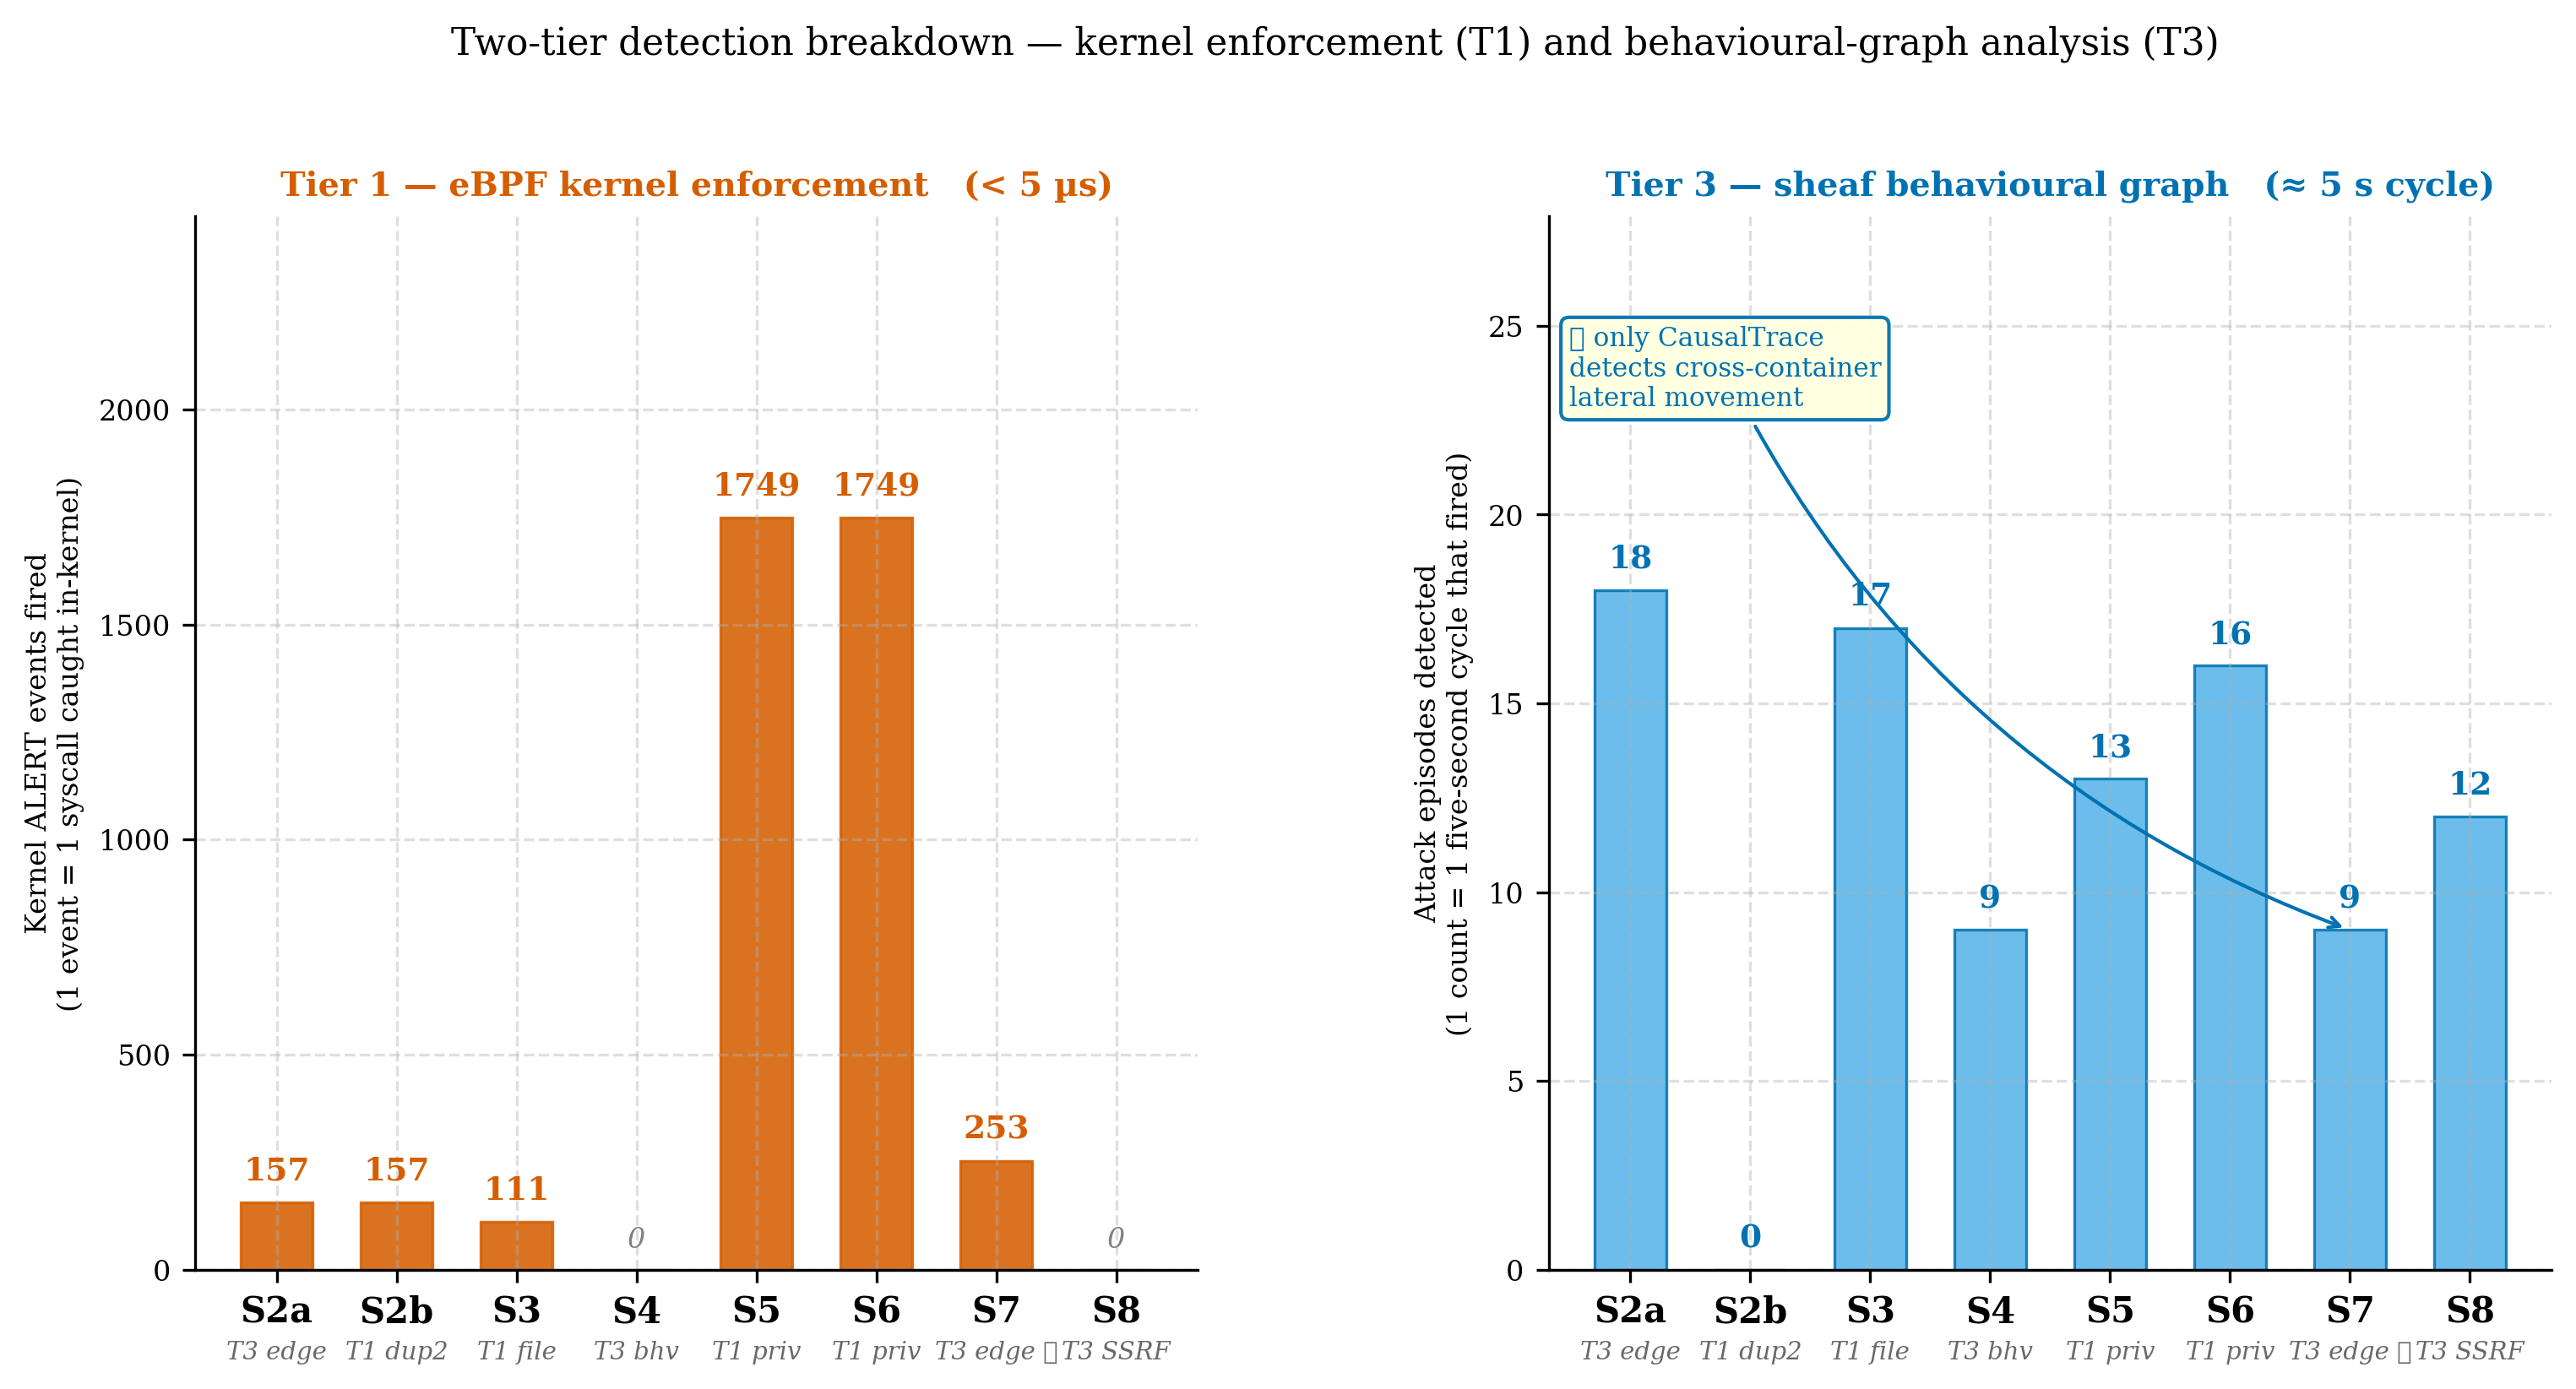
\includegraphics[width=\linewidth]{figures/fig_tier_breakdown.png}
  \caption[Tier breakdown per scenario]{Per-scenario detection
  attribution by tier. Tier-1 dominates the in-container classes;
  Tier-3 dominates the cross-container and chain classes. The two
  surfaces cover complementary subsets of the attack space.}
  \label{fig:tier-breakdown}
\end{figure}

\begin{figure}[t]
  \centering
  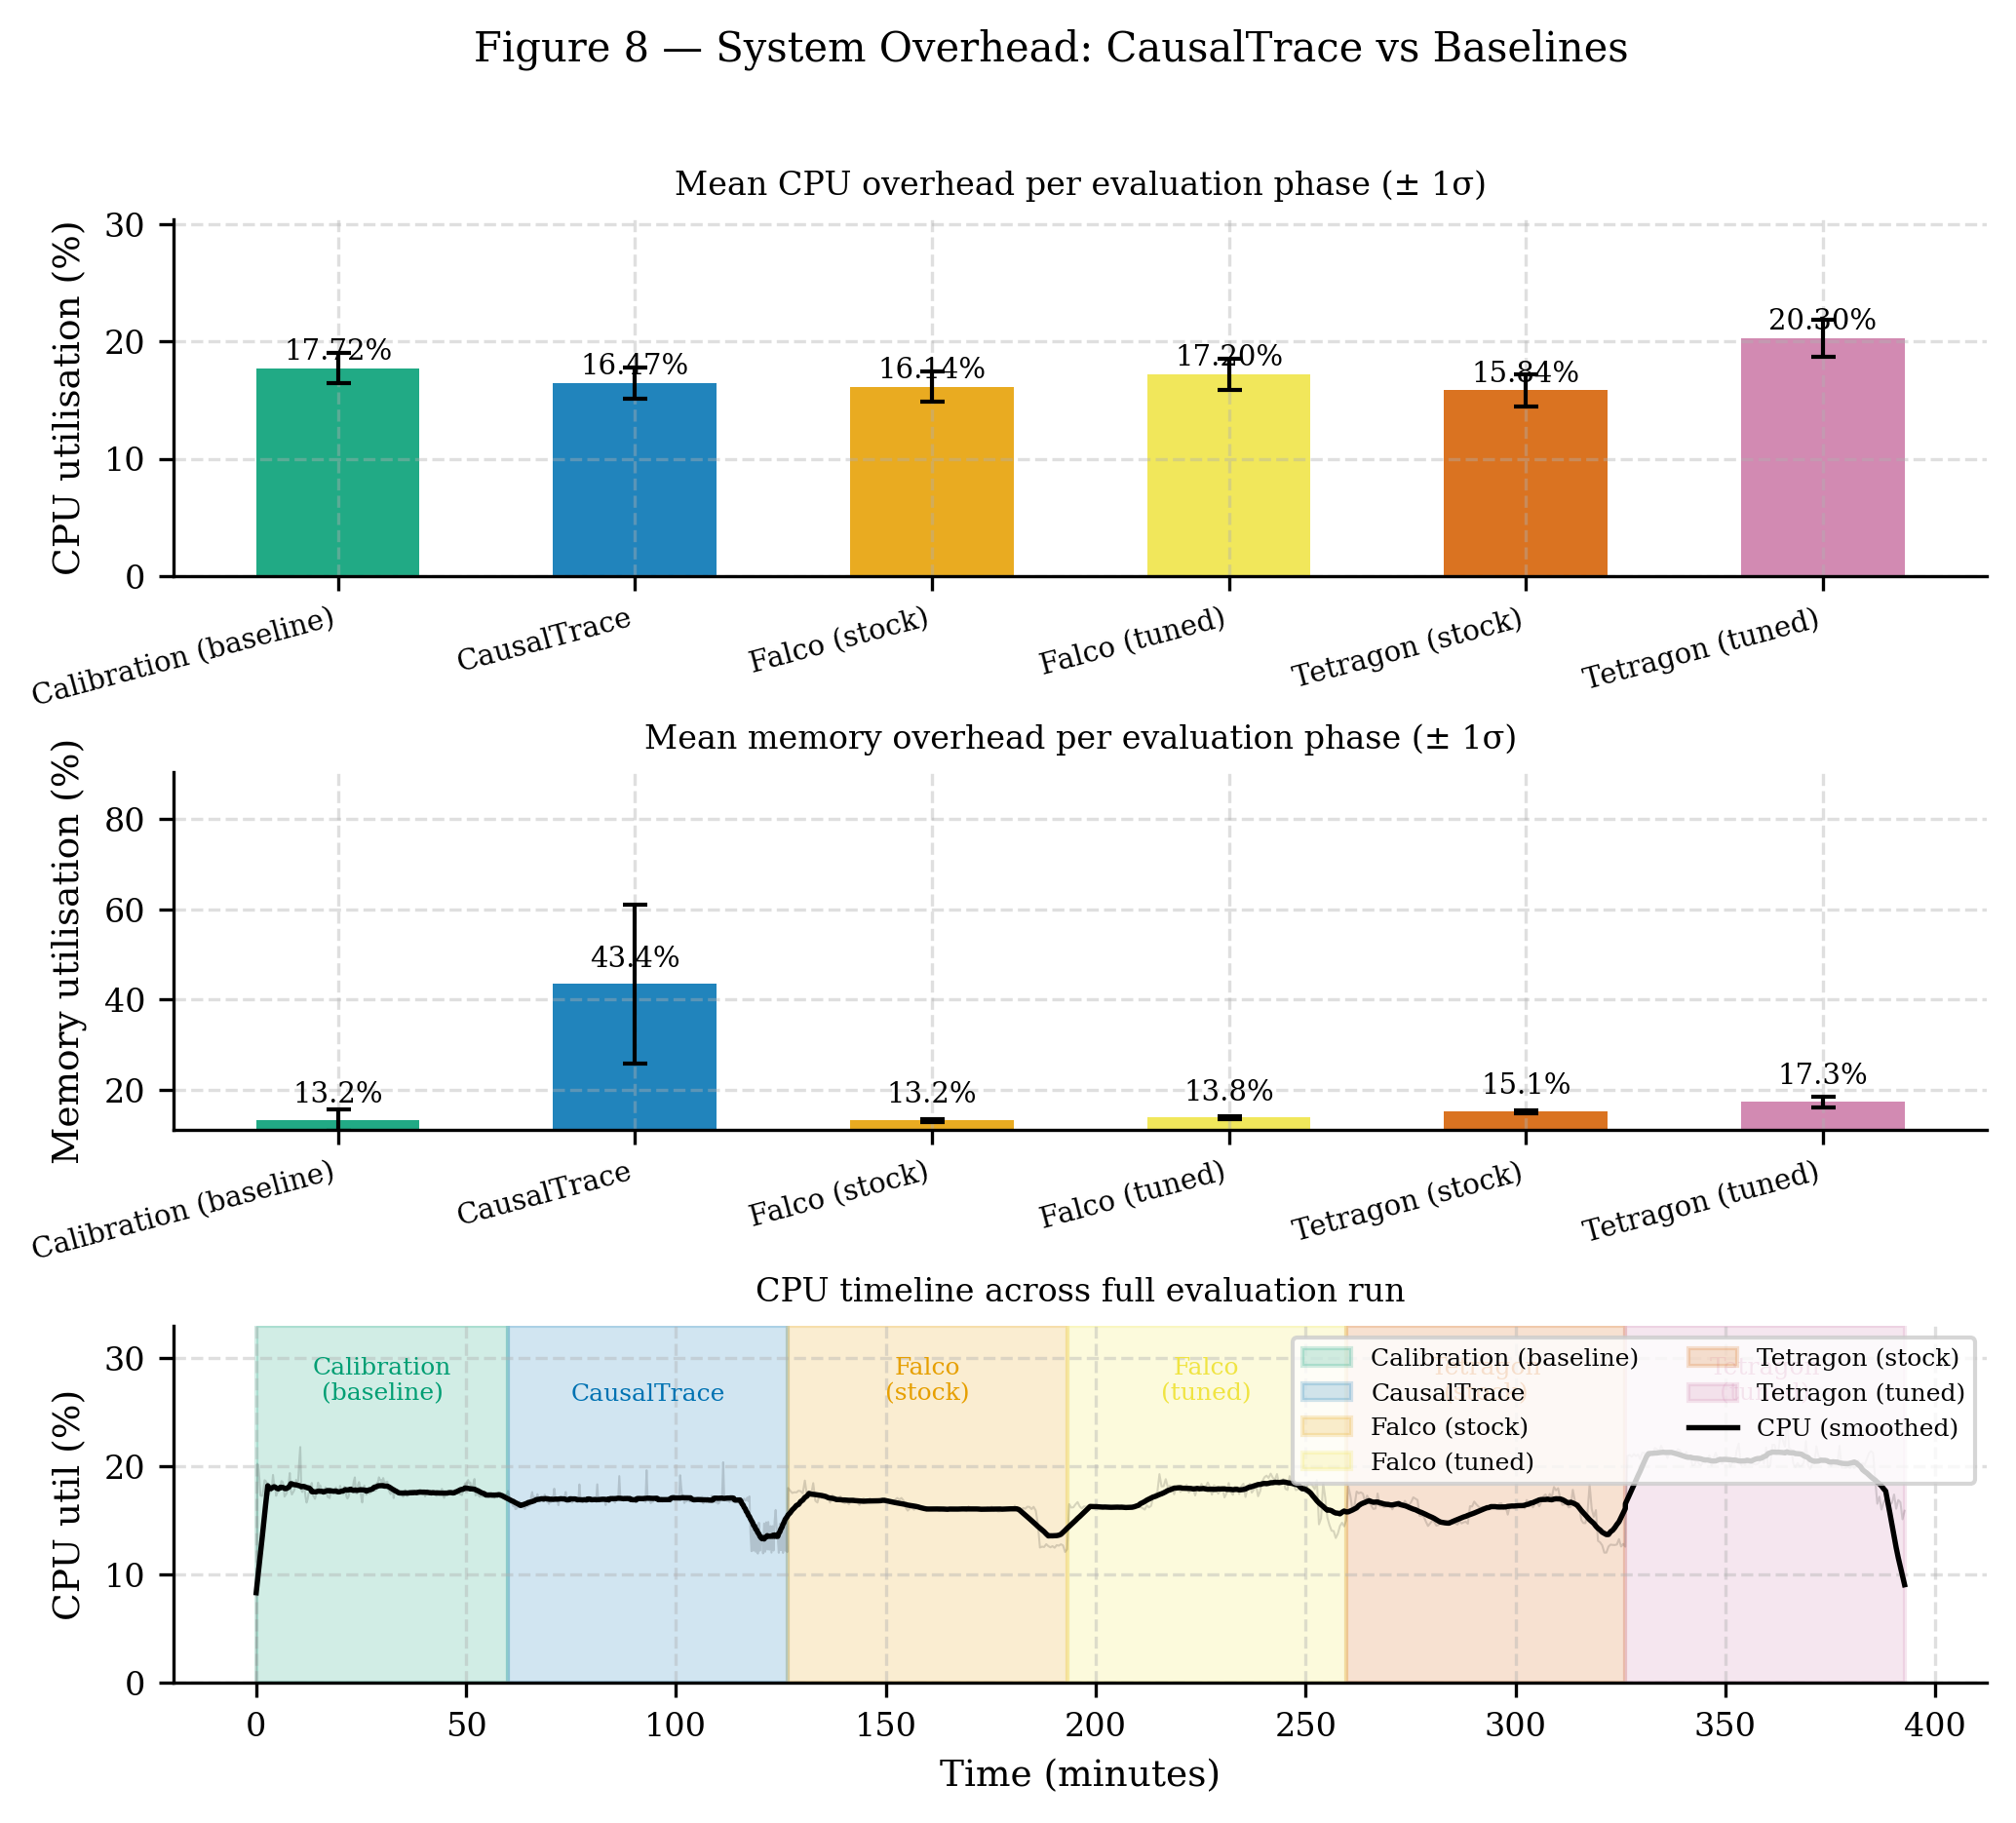
\includegraphics[width=\linewidth]{figures/fig_runtime_overhead.png}
  \caption[Runtime overhead]{Runtime overhead on a \texttt{wrk}-driven
  load against ct-nginx. CausalTrace's $\approx 1\,\%$ throughput impact
  is dominated by the \texttt{bpf\_probe\_read\_kernel} indirection
  forced by the verifier workaround of Chapter~\ref{Chapter5}.}
  \label{fig:runtime-overhead}
\end{figure}

%─────────────────────────────────────────────────────────────────────────────
\section{Threats to validity}
\label{sec:threats}
%─────────────────────────────────────────────────────────────────────────────

Four threats shape how these results should be read. Cross-kernel
generalisation is plausible but unverified: all results come from a
single evaluation host on Linux~6.17, and the verifier workarounds of
Chapter~\ref{Chapter5} are kernel-version-specific. Testbed realism is
bounded: the 22-container mesh reproduces a realistic service graph but
the workload generated by \texttt{wrk} and docker-exec is synthetic.
Baseline tuning introduces a pro-CausalTrace bias: we tuned Falco and
Tetragon for this attack set, which is also the set CausalTrace is
designed to catch, so stock numbers under-count what a production Falco
operator would write. Finally, the Wilson interval at $\hat{p}=1.00$
with $n=15$ per scenario has lower bound $\approx 0.80$, so a scenario
reporting 15/15 could plausibly be an 80\,\% detector; aggregate
intervals across the 155-injection set are much tighter.
 
\chapter{Conclusion}
\label{Chapter7}
\lhead{Chapter 7. \emph{Conclusion}}

%─────────────────────────────────────────────────────────────────────────────
\section{Summary}
\label{sec:conclusion-summary}
%─────────────────────────────────────────────────────────────────────────────

CausalTrace defends a container cluster on two surfaces. The kernel
surface enforces physical invariants---a process whose standard input
points to a socket is a reverse shell regardless of how it got there. The
coupling surface observes inter-container behaviour as a cellular sheaf
whose Rayleigh quotient rises when the graph of service interactions
violates its calibrated structure. The two surfaces are independent; a
failed Tier-3 daemon never disables Tier-1 enforcement.

Four claims distinguish the work. The \emph{three-tier architecture with
an independence invariant} separates the hot path from the analytics
path. The \emph{compound enforcement gate with a four-level trust model}
replaces the binary kill/allow decision with a three-case taxonomy gated
by per-IP trust, and uses a TC classifier to drop only the attacker's
packets at the veth. The \emph{rank-$15$ CCA calibration pipeline}
produces a finite, well-conditioned coupling model on realistic windows
where the earlier $k{=}50$ iteration was rank-deficient. The
\emph{seed-reproducible evaluation harness} replays an identical
155-injection sequence against every detector under the same workload;
the resulting headline numbers are CausalTrace 99.4\,\% [96, 100],
Falco tuned 70.3\,\% [63, 77], Tetragon tuned 1.3\,\% [0, 5].

%─────────────────────────────────────────────────────────────────────────────
\section{Limitations}
\label{sec:conclusion-limitations}
%─────────────────────────────────────────────────────────────────────────────

Five limitations bound the results. \emph{Host root compromises the
defender}; CausalTrace is kernel-resident, and an attacker with host root
can unload the BPF programs. \emph{Results come from a single evaluation
host} on Linux~6.17, so cross-kernel generalisation remains unverified.
\emph{Probe~B is IPv4-only}; deployments with IPv6-first meshes need an
additional \texttt{tcp\_v6\_connect} hook. \emph{The trust model is
pessimistic for accept-thread-plus-thread-pool servers}, where per-TID
attribution falls back to the per-cgroup best-effort path. \emph{Baseline
tuning introduces a pro-CausalTrace bias}: Falco and Tetragon were tuned
for this attack set, and a production Falco operator would invest more
effort than our tuned ruleset reflects.

%─────────────────────────────────────────────────────────────────────────────
\section{Future work}
\label{sec:conclusion-future}
%─────────────────────────────────────────────────────────────────────────────

Each limitation flows to an extension.

\paragraph{Multi-host sheaf.} The cellular sheaf construction extends to
a bipartite graph with intra-host edges (the current case) and inter-host
edges (flow-level attributions between hosts). A distributed calibrator
that synchronises restriction maps per inter-host edge plus a gossip
protocol for burn-list synchronisation would lift CausalTrace from
single-node to cluster scale without new mathematics.

\paragraph{Incremental online calibration.} A rolling window that updates
the restriction maps under the same six-cycle pristine-streak rule the
guarded EMA already uses (Section~\ref{sec:ema}) would remove the
calibration barrier and let the system track workload drift without an
offline pass.

\paragraph{IPv6 and accept-thread attribution.} Both are engineering
extensions rather than research; the \texttt{tcp\_v6\_connect} hook is a
one-day patch, and a thread-pool-aware attribution path would require
the dispatcher to consult a per-thread-pool client-IP map populated by
the accept-thread itself.

\paragraph{Hardware offload for the TC classifier.} Moving the
\texttt{drop\_ip\_list} consultation into smart-NIC XDP offload would cut
per-packet cost from $\approx\!100$\,ns to sub-10\,ns and reduce CPU
load during a sustained attack.

\paragraph{Formal verification of the compound gate.} The three-case
taxonomy is stated informally in Section~\ref{sec:compound}. A formal
model in a proof assistant would let us prove invariants such as
``every Case-A trigger either burns the attacker's trust or issues a
SIGKILL'' and ``the gate never kills a calibrated client without a
Case-A invariant''. The gate is under 100 lines of C; verification is
tractable.

%─────────────────────────────────────────────────────────────────────────────
\section{Closing remarks}
\label{sec:conclusion-closing}
%─────────────────────────────────────────────────────────────────────────────

Container runtime security is a crowded field. What distinguishes
CausalTrace is the commitment to a two-surface formulation: strict
physical invariants enforced at the kernel boundary, plus a mathematical
model of inter-container coupling that detects the composite attacks no
single-container rule catches. The mathematics is classical---CCA,
Mahalanobis distance, cellular sheaves, count-min sketches. The
engineering is kernel-resident---a tail-call dispatcher, six specialist
handlers, TC direct-action classifiers, a compound gate with an explicit
three-case taxonomy.

The demonstration is that the two surfaces, composed carefully, are both
faster and more discriminating than the best-available production
tooling on the attack classes this field cares about. Whether the
system is \emph{deployable} is a question for operators and for the
extensions above. Whether it \emph{works} is answered in
Chapter~\ref{Chapter6}.
 

%----------------------------------------------------------------------------------------
%THESIS CONTENT - APPENDICES
%----------------------------------------------------------------------------------------
\addtocontents{toc}{\vspace{2em}} 
\appendix 
\chapter{Attack Scenarios}
\label{AppendixA}
\lhead{Appendix A. \emph{Attack Scenarios}}

Table~\ref{tab:attack-catalogue} catalogues the thirteen attack scripts
(eleven scenarios plus two evasion variants) driven from
\texttt{ct\_attacker} against \texttt{ct\_prod\_net} during the marathon
evaluation. S1 is the normal-traffic negative control. S11 is the
held-out out-of-distribution injection. Every script lives under
\texttt{attacks/} and is invoked by
\texttt{run\_marathon\_evaluation.py}.

\begin{table}[h]
\centering
\caption[Attack catalogue]{Attack scenarios, kernel primitive, catching
handler, and MITRE~ATT\&CK ID. S2a and S3a add noise-syscall padding to
dilute the bigram sketch; Theorem~\ref{thm:bigram} shows why the padding
does not help the attacker.}
\label{tab:attack-catalogue}
\footnotesize
\setlength\tabcolsep{3pt}
\begin{tabular}{@{}l l p{4.8cm} l l@{}}
\toprule
ID & Script (\texttt{attacks/scenario\_\ldots}) & Kernel primitive & Tier-1 handler & MITRE \\
\midrule
S1   & \texttt{1\_normal}           & \texttt{curl/wrk} requests                  & ---                           & neg. \\
S2   & \texttt{2\_reverse\_shell}   & \texttt{dup2(sock, 0|1|2)}                   & \texttt{handle\_dup2}         & T1059 \\
S2a  & \texttt{2a\_evade}           & \texttt{dup2(sock,0|1|2)} + syscall-noise pad & \texttt{handle\_dup2}       & T1059 \\
S3   & \texttt{3\_sensitive\_file}  & \texttt{openat("/etc/shadow")}               & \texttt{handle\_file}         & T1552 \\
S3a  & \texttt{3\_evade}            & \texttt{openat("/etc/sha*")} + syscall-noise pad & \texttt{handle\_file}    & T1552 \\
S4   & \texttt{4\_fork\_bomb}       & $d^2\!>\!0$ clone burst                     & \texttt{handle\_fork}         & T1499 \\
S5   & \texttt{5\_ns\_escape}       & \texttt{nsenter}\,$\to$\,\texttt{setns(fd,\_NEWNS)} & \texttt{handle\_privesc} & T1611 \\
S6   & \texttt{6\_privesc}          & \texttt{unshare}\,+\,\texttt{setuid(0)}              & \texttt{handle\_privesc} & T1620 \\
S7   & \texttt{7\_cross\_container} & lateral \texttt{connect} + foothold         & \texttt{trace\_connect\_ret}  & T1021 \\
S8   & \texttt{8\_log4shell}        & JNDI \texttt{ldap://} $\to$ shell           & \texttt{handle\_execve}       & T1190 \\
S9   & \texttt{9\_ssrf\_rce}        & SSRF $\to$ pivot $\to$ RCE                  & Tier-3 sheaf edge             & T1068 \\
S10  & \texttt{10\_container\_escape} & rare-syscall chain (\texttt{unshare}, \texttt{mount},
                                          \texttt{memfd}, \texttt{bpf})
                                                                                & \texttt{handle\_privesc} + Top-24 & T1611 \\
S11  & \texttt{11\_fileless\_memfd} & \texttt{memfd\_create}+\texttt{execveat}    & \texttt{handle\_execve}       & T1055 \\
\bottomrule
\end{tabular}
\end{table}

MITRE identifiers: T1059~\cite{mitre_t1059}, T1552~\cite{mitre_t1552},
T1611~\cite{mitre_t1611}, T1620~\cite{mitre_t1620},
T1021~\cite{mitre_t1021}. T1499/T1190/T1068/T1055 are additional ATT\&CK
technique IDs from the MITRE catalogue~\cite{mitre2024attack}.

Scenarios S2a, S3a, and S11 are designed to evade the frequency-based
detector a na\"ive bigram-only system would use. S2a performs the
reverse-shell \texttt{dup2} sequence but interleaves bursts of noise
syscalls (\texttt{getpid}, \texttt{gettid}, \texttt{clock\_gettime}) to
dilute the attacker's bigram signal toward uniform. S3a does the same
with the sensitive-file read: \texttt{openat("/etc/shadow")} plus
surrounding noise bursts to dilute the CMS. Both attacks defeat any
frequency-only detector, yet Tier-1's invariant handlers still fire
because the strict contract violation (socket fd in stdio slots,
path prefix match on \texttt{/etc/sha*}) is orthogonal to bigram
frequency. S11 stages the payload through \texttt{memfd\_create} and
runs it via \texttt{execveat} on \texttt{/proc/self/fd/N}---a path
class the calibrator has never seen, stressing the OOD capability of
the \texttt{handle\_execve} path-class check.

Full scripts are reproduced verbatim in the repository under
\texttt{attacks/}; the injection harness is
\texttt{run\_marathon\_evaluation.py}.

\chapter{Key BPF Map Layouts}
\label{AppendixB}
\lhead{Appendix B. \emph{BPF Map Layouts}}

This appendix records the exact schema of every BPF map that the Tier-1
handlers, Tier-2 probes, and Tier-3 daemon share. Table~\ref{tab:bpf-maps-full}
gives the full reference; the three \texttt{struct} layouts that carry
non-trivial fields are reproduced inline below the table.

\begin{table}[h]
\centering
\caption[Full BPF map schema]{Complete BPF map schema. Keys and values
are the bytes stored in the map; see the structure definitions below
the table for the non-trivial \texttt{struct}-valued maps. Size columns
give the map capacity in entries (or in bytes for ring buffers).}
\label{tab:bpf-maps-full}
\footnotesize
\setlength\tabcolsep{3pt}
\begin{tabular}{@{}l l l l r@{}}
\toprule
Map                          & Type                 & Key      & Value                          & Size \\
\midrule
\texttt{host\_ns}            & \texttt{ARRAY}       & \texttt{u32}  & \texttt{u32}                       & 1 \\
\texttt{prog\_array}         & \texttt{PROG\_ARRAY} & \texttt{u32}  & prog fd                            & 512 \\
\texttt{bigram\_sketch\_map} & \texttt{HASH}        & \texttt{u64}  & \texttt{u32[512]} CMS             & 256 \\
\texttt{container\_behavior} & \texttt{HASH}        & \texttt{u64}  & \texttt{struct behavior\_state}   & 256 \\
\texttt{rate\_map}           & \texttt{HASH}        & \texttt{u64}  & \texttt{struct rate\_state}       & 256 \\
\texttt{pending\_cgroup\_inherit} & \texttt{HASH}   & \texttt{u32}  & \texttt{u64}                      & 128 \\
\texttt{client\_trust}       & \texttt{HASH}        & \texttt{u32}  & \texttt{u8}                       & 4096 \\
\texttt{tid\_client\_ip}     & \texttt{LRU\_HASH}   & \texttt{u64}  & \texttt{u32}                      & 16384 \\
\texttt{cgroup\_current\_client} & \texttt{HASH}    & \texttt{u64}  & \texttt{u32}                      & 256 \\
\texttt{connection\_context} & \texttt{LRU\_HASH}   & sock~ptr      & \texttt{struct conn\_context}     & 8192 \\
\texttt{connect\_sk\_stash}  & \texttt{LRU\_HASH}   & \texttt{u64}  & sock~ptr                           & 4096 \\
\texttt{ip\_to\_cgroup}      & \texttt{HASH}        & \texttt{u32}  & \texttt{u64}                       & 256 \\
\texttt{drop\_ip\_list}      & \texttt{HASH}        & \texttt{u32}  & \texttt{u64}~(expiry\,ns)          & 4096 \\
\texttt{alerts\_rb}          & \texttt{RINGBUF}     & --            & \texttt{struct alert\_t}           & 64\,K \\
\texttt{telemetry\_rb}       & \texttt{RINGBUF}     & --            & \texttt{struct telemetry\_t}       & 256\,K \\
\texttt{verdict\_map}        & \texttt{HASH}        & \texttt{u64}  & \texttt{u32}~(KILL/ALLOW)          & 256 \\
\texttt{enforce\_level\_map} & \texttt{HASH}        & \texttt{u64}  & \texttt{struct enforce\_state}    & 256 \\
\texttt{deny\_connect\_map}  & \texttt{HASH}        & \texttt{u64}  & \texttt{u32}~(errno)               & 1024 \\
\texttt{deny\_open\_map}     & \texttt{HASH}        & \texttt{u64}  & \texttt{u32}                       & 256 \\
\texttt{deny\_exec\_map}     & \texttt{HASH}        & \texttt{u64}  & \texttt{u32}                       & 256 \\
\texttt{rate\_limit\_map}    & \texttt{HASH}        & \texttt{u64}  & \texttt{struct rate\_limit\_state}& 256 \\
\texttt{fw\_allow\_map}      & \texttt{HASH}        & \texttt{u64}  & \texttt{u32}                       & 512 \\
\texttt{tc\_stats}           & \texttt{ARRAY}       & \texttt{u32}  & \texttt{u64}                       & 8 \\
\bottomrule
\end{tabular}
\end{table}

\section*{Key \texttt{struct} layouts}

\textbf{\texttt{behavior\_state}} — per-cgroup behaviour bitfield plus per-bit
timestamps.
\begin{verbatim}
struct behavior_state {
    u64 flags;         /* 8 BIT_* flags */
    u64 bit_ts[8];     /* ns timestamp per bit */
    u64 conn_dst_cg;   /* last lateral connect dst */
    u16 conn_port;     /* last lateral connect port */
    u16 _pad[3];
};
\end{verbatim}
The eight bits are \texttt{BIT\_SHELL\_SPAWN}, \texttt{BIT\_LATERAL\_CONNECT},
\texttt{BIT\_SENSITIVE\_FILE}, \texttt{BIT\_NS\_PROBE},
\texttt{BIT\_PRIVESC}, \texttt{BIT\_LARGE\_TRANSFER},
\texttt{BIT\_FD\_REDIRECT}, and \texttt{BIT\_FORK\_ACCEL}.

\textbf{\texttt{rate\_state}} — per-cgroup fork rate window with state for
the discrete second derivative.
\begin{verbatim}
struct rate_state {
    u64 window_start;  /* ns */
    u64 count;
    u64 prev_count;
    u64 prev_prev_count;
};
\end{verbatim}
The fork handler computes $d^2 = \mathrm{count} - 2\cdot\mathrm{prev} +
\mathrm{prev\_prev}$ to separate exponential growth (fork bomb) from
linear bursts (\texttt{make -j}).

\textbf{\texttt{conn\_context}} — per-socket byte accumulator used by the
L4-stability trust-promotion gate.
\begin{verbatim}
struct conn_context {
    u32 client_ip;
    u64 bytes_in;
    u64 bytes_out;
    u64 first_seen_ns;
    u64 last_seen_ns;
};
\end{verbatim}

\textbf{\texttt{enforce\_state}} — graduated L0--L6 level with TTL so
enforcement self-expires.
\begin{verbatim}
struct enforce_state {
    u32 level;         /* 0..6 */
    u64 expiry_ns;
    u32 rule_count;
};
\end{verbatim}

All other maps store primitive keys and values as indicated in
Table~\ref{tab:bpf-maps-full}; their schemas require no further
explanation.

\chapter{Reproduction Recipe}
\label{AppendixC}
\lhead{Appendix C. \emph{Reproduction Recipe}}

Every quantitative result in Chapter~\ref{Chapter6} is regenerated by
the command sequence below on a clean Ubuntu~24.04 host running Linux
kernel~6.17 and BCC~0.31. The full run is driven by the project
\texttt{Makefile}; each target below maps to one step.

\begin{verbatim}
# 1. Prerequisites (one-time)
$ sudo apt-get install -y build-essential bpfcc-tools \
      python3-bpfcc iproute2 docker.io docker-compose-v2 wrk falco
$ python3 -m venv .venv && source .venv/bin/activate
$ pip install -r requirements.txt

# 2. Bring the 22-container testbed up
$ make up                                 # docker compose up + routes

# 3. Calibrate (writes calibration/*.npz, *.pkl, *.json)
$ make calibrate

# 4. Full marathon (CausalTrace + Falco stock/tuned + Tetragon stock/tuned,
#    one seed-42 permutation of 155 attacks replayed per detector)
$ make marathon

# 5. Analyse and regenerate every paper figure + Wilson-CI table
$ python3 scripts/marathon_analyze.py results/marathon
$ python3 generate_astar_plots.py --data-dir results/marathon \
      --out-dir BTech_Project_Report/figures
$ python3 BTech_Project_Report/figures/build_detection_table.py

# 6. Rebuild the thesis PDF
$ cd BTech_Project_Report && pdflatex main && bibtex main && \
      pdflatex main && pdflatex main
\end{verbatim}

The seeded attack permutation is stored in
\texttt{results/marathon/state.json}; resumable runs use
\texttt{run\_marathon\_evaluation.py --resume}. The detection-window
width ($\Delta = 25$\,s) and the CCA rank ($k = 15$) are the only
hyper-parameters that need to be kept consistent between calibration and
evaluation; everything else is data-driven.


\addtocontents{toc}{\vspace{2em}} % Add a gap in the Contents, for aesthetics

\backmatter

%----------------------------------------------------------------------------------------
%BIBLIOGRAPHY
%----------------------------------------------------------------------------------------
\nocite{*}
\label{Bibliography}

\lhead{\emph{Bibliography}} % Change the page header to say "Bibliography"

\bibliographystyle{IEEEtran} % Use the "custom" BibTeX style for formatting the Bibliography

\bibliography{Bibliography} % The references (bibliography) information are stored in the file named "Bibliography.bib"

\end{document}  